%%%%%% Run at command line, run
%%%%%% xelatex grad-sample.tex 
%%%%%% for a few times to generate the output pdf file
\documentclass[12pt,oneside,openright,a4paper]{cpe-english-project}

\usepackage{polyglossia}
\usepackage{tabularx}
\usepackage{float}
%\usepackage{algorithm}
\setdefaultlanguage{english}
\setotherlanguage{thai}
\newfontfamily\thaifont[Script=Thai,Scale=1.23]{TH Sarabun New}
\defaultfontfeatures{Mapping=tex-text,Scale=1.0,LetterSpace=0.0}
\setmainfont[Scale=1.0,LetterSpace=0,WordSpace=1.0,FakeStretch=1.0]{Times New Roman}

% Custom setting
\parindent=3em
\setlength{\parskip}{1em} % Set paragraph margin
% Set nested numuric list
\renewcommand{\labelenumii}{\theenumii}
\renewcommand{\theenumii}{\theenumi.\arabic{enumii}.}
\renewcommand{\labelenumiii}{\theenumiii}
\renewcommand{\theenumiii}{\theenumii.\arabic{enumiii}.}
% End set nested numuric list
% Caption with source
%\usepackage[justification=centering]{caption}
\newcommand*{\captionsource}[2]{%
  \caption[{#1}]{#1}\vspace{-8pt}
  \textbf{Source:} #2}
\newenvironment{blockquote}{%
  \par%
  \medskip
  \leftskip=4em\rightskip=2em%
  \noindent\ignorespaces}{%
  \par\medskip}
\let\oldquote\quote
\let\endoldquote\endquote

\RenewDocumentEnvironment{quote}{om}
  {\oldquote}
  {\par\nobreak\smallskip
   \hfill(#2\IfValueT{#1}{~---~#1})\endoldquote 
   \addvspace{\bigskipamount}}
% Code
\usepackage{listings}
\usepackage{color}

\definecolor{dkgreen}{rgb}{0,0.6,0}
\definecolor{gray}{rgb}{0.5,0.5,0.5}
\definecolor{mauve}{rgb}{0.58,0,0.82}
\lstset{frame=tb,
  language=Python,
  aboveskip=3mm,
  belowskip=3mm,
  showstringspaces=false,
  columns=flexible,
  basicstyle={\small\ttfamily},
  numbers=none,
  numberstyle=\tiny\color{gray},
  keywordstyle=\color{blue},
  commentstyle=\color{dkgreen},
  stringstyle=\color{mauve},
  breaklines=true,
  breakatwhitespace=true,
  tabsize=3
}
%\setmathfont(Digits)[Scale=1.0,LetterSpace=0,FakeStretch=1.0]{Times New Roman}


%%%%%%%%%%%%%%%%%%%%%%%%%%%%%%%%%%%%%%%%%%%%%%%%%%%%%%%%%%%%%%%%%%%
% Customize below to suit your needs 
% The ones that are optional can be left blank. 
%%%%%%%%%%%%%%%%%%%%%%%%%%%%%%%%%%%%%%%%%%%%%%%%%%%%%%%%%%%%%%%%%%%
% First line of title
\def\disstitleone{PROJECT NO. 72}   
% Second line of title
\def\disstitletwo{A RESTAURANT RECOMMENDATION SYSTEM FOR INDIVIDUALS AND GROUPS}   
% Your first name and lastname
\def\dissauthor{MR. CHANCHANA WICHA}   % 1st member
\def\dissauthortwo{MS. IRIN YOOKTAJARONG}   % 2nd member (optional)
\def\dissauthorthree{}


% The degree that you're persuing..
\def\dissdegree{Bachelor of Engineering} % Name of the degree
\def\dissdegreeabrev{B.Eng} % Abbreviation of the degree
\def\dissyear{2020}                   % Year of submission
\def\thaidissyear{2563}               % Year of submission (B.E.)

%%%%%%%%%%%%%%%%%%%%%%%%%%%%%%%%%%%%%%%%%%%%
% Your project and independent study committee..
%%%%%%%%%%%%%%%%%%%%%%%%%%%%%%%%%%%%%%%%%%%%
\def\dissadvisor{Dr. Unchalisa Taetragool, Ph.D.}  % Advisor
%%% Leave it empty if you have no Co-advisor
\def\disscoadvisor{}  % Co-advisor
\def\disscommitteetwo{Asst.Prof.Dr. Rajchawit Sarochawikasit, Ph.D.}  % 3rd committee member (optional)
\def\disscommitteethree{Dr. Sally E. Goldin, Ph.D.}   % 4th committee member (optional) 
\def\disscommitteefour{Asst.Prof.Mr. Sanan Srakaew, B.Eng.}    % 5th committee member (optional) 

\def\worktype{Project} %%  Project or Independent study
\def\disscredit{3}   %% 3 credits or 6 credits


\def\fieldofstudy{Computer Engineering} 
\def\department{Computer Engineering} 
\def\faculty{Engineering}

\def\thaifieldofstudy{วิศวกรรมคอมพิวเตอร์} 
\def\thaidepartment{วิศวกรรมคอมพิวเตอร์} 
\def\thaifaculty{วิศวกรรมศาสตร์}
 
\def\appendixnames{Appendix} %%% Appendices or Appendix

\def\thaiworktype{ปริญญานิพนธ์} %  Project or research project % 
\def\thaidisstitleone{หัวข้อปริญญานิพนธ์บรรทัดแรก}
\def\thaidisstitletwo{หัวข้อปริญญานิพนธ์บรรทัดสอง}
\def\thaidissauthor{นายชาญชนะ วิชา}
\def\thaidissauthortwo{นางสาวไอริณ ยุกตจรงค์} %Optional
\def\thaidissauthorthree{} %Optional

\def\thaidissadvisor{ดร. อัญชลิสา แต้ตระกูล}
%% Leave this empty if you have no co-advisor
\def\thaidisscoadvisor{} %Optional
\def\thaidissdegree{วิศวกรรมศาสตรบัณฑิต}

% Change the line spacing here...
\linespread{1.15}

%%%%%%%%%%%%%%%%%%%%%%%%%%%%%%%%%%%%%%%%%%%%%%%%%%%%%%%%%%%%%%%%
% End of personal customization.  Do not modify from this part 
% to \begin{document} unless you know what you are doing...
%%%%%%%%%%%%%%%%%%%%%%%%%%%%%%%%%%%%%%%%%%%%%%%%%%%%%%%%%%%%%%%%


%%%%%%%%%%%% Dissertation style %%%%%%%%%%%
%\linespread{1.6} % Double-spaced  
%%\oddsidemargin    0.5in
%%\evensidemargin   0.5in
%%%%%%%%%%%%%%%%%%%%%%%%%%%%%%%%%%%%%%%%%%%
%\renewcommand{\subfigtopskip}{10pt}
%\renewcommand{\subfigbottomskip}{-5pt} 
%\renewcommand{\subfigcapskip}{-6pt} %vertical space between caption
%                                    %and figure.
%\renewcommand{\subfigcapmargin}{0pt}

\renewcommand{\topfraction}{0.85}
\renewcommand{\textfraction}{0.1}

\newtheorem{theorem}{Theorem}
\newtheorem{lemma}{Lemma}
\newtheorem{corollary}{Corollary}

\def\QED{\mbox{\rule[0pt]{1.5ex}{1.5ex}}}
\def\proof{\noindent\hspace{2em}{\itshape Proof: }}
\def\endproof{\hspace*{\fill}~\QED\par\endtrivlist\unskip}
%\newenvironment{proof}{{\sc Proof:}}{~\hfill \blacksquare}
%% The hyperref package redefines the \appendix. This one 
%% is from the dissertation.cls
%\def\appendix#1{\iffirstappendix \appendixcover \firstappendixfalse \fi \chapter{#1}}
%\renewcommand{\arraystretch}{0.8}
%%%%%%%%%%%%%%%%%%%%%%%%%%%%%%%%%%%%%%%%%%%%%%%%%%%%%%%%%%%%%%%%
%%%%%%%%%%%%%%%%%%%%%%%%%%%%%%%%%%%%%%%%%%%%%%%%%%%%%%%%%%%%%%%%


\begin{document}
\pdfstringdefDisableCommands{%
\let\MakeUppercase\relax
}
\begin{center}
  
\includegraphics[width=2.8cm]{logo02.jpg}
\end{center}
\vspace*{-1cm}

\maketitlepage
\makesignaturepage 

%%%%%%%%%%%%%%%%%%%%%%%%%%%%%%%%%%%%%%%%%%%%%%%%%%%%%%%%%%%%%%
%%%%%%%%%%%%%%%%%%%%%% English abstract %%%%%%%%%%%%%%%%%%%%%%%
%%%%%%%%%%%%%%%%%%%%%%%%%%%%%%%%%%%%%%%%%%%%%%%%%%%%%%%%%%%%%%
\abstract

In recent years, recommendation systems are widely used for movies, music, or products in order to reduce the time and effort of the users’ searching and increase users’ experience. However, restaurant recommendation systems are still very few in this industry and the existing recommenders in Thailand are just randomization applications and the majority of recommender systems are designed for individual users. In contrast, since this activity or event usually occurs in a group of people, not just individually, which each person can have the same or different behaviors, preferences, and interests. Therefore, group decisions often differ from individual decisions. As a result, each decision is often taken longer than one person, and sometimes conclusions are not able to be drawn or it may cause conflicts within the group.

According to the mentioned problems, we were motivated to develop this project, A Restaurant Recommendation System for Individuals and Groups, to better assist in group decision making. Our project is a web application that recommends restaurants in the Bangkok area to users based on their behaviors, preferences, and interests of both individuals and groups eating. The genetic algorithm is applied for generating suitable recommended restaurants for users. Therefore, this project aims to reduce time-wasting of decision making for both individuals and groups and increase the users’ experience and satisfaction when using our recommendation system.


\begin{flushleft}
\begin{tabular*}{\textwidth}{@{}lp{0.8\textwidth}}
\textbf{Keywords}: & Genetic Algorithm / Optimization Problem / Decision Making Process / Group Recommendation Systems / Web Application / Restaurants
\end{tabular*}
\end{flushleft}
\endabstract

%%%%%%%%%%%%%%%%%%%%%%%%%%%%%%%%%%%%%%%%%%%%%%%%%%%%%%%%%%%%%%
%%%%%%%%%% Thai abstract here %%%%%%%%%%%%%%%%%%%%%%%%%%%%%%%%%
%%%%%%%%%%%%%%%%%%%%%%%%%%%%%%%%%%%%%%%%%%%%%%%%%%%%%%%%%%%%%%
{
\XeTeXlinebreaklocale "th_TH"	
\thaifont
\thaiabstract

ในช่วงไม่กี่ปีที่ผ่านมาได้มีการใช้ระบบแนะนำ (Recommendation System) อย่างแพร่หลายไม่ว่าจะเป็นภาพยนตร์ เพลง หรือระบบแนะนำผลิตภัณฑ์ต่าง ๆ เพื่อลดระยะเวลาและความยุ่งยากในการค้นหาของผู้ใช้รวมถึงเพิ่มประสบการณ์ของผู้ใช้อย่างไรก็ตามระบบแนะนำร้านอาหารยังมีน้อยมากในวงการระบบคำแนะนำนอกจากนั้นระบบแนะนำร้านอาหารที่มีอยู่ในประเทศไทยเป็นเพียงแอปพลิเคชันแบบสุ่มและส่วนใหญ่ออกแบบมาสำหรับผู้ใช้แต่ละรายเท่านั้น ซึ่งในความเป็นจริงแล้วการรับประทานอาหารมักเกิดขึ้นเป็นกลุ่มตั้งแต่ 2 คนขึ้นไปไม่ได้เป็นรายบุคคลเพียงอย่างเดียว ซึ่งแต่ละคนในกลุ่มนั้นมีพฤติกรรม ความชอบและความสนใจที่อาจจะเหมือนหรือแตกต่างกันดังนั้นการตัดสินใจของกลุ่มมักแตกต่างจากการตัดสินใจของแต่ละบุคคล ด้วยเหตุนี้การตัดสินใจในแต่ละครั้ง มักใช้เวลานานกว่าการตัดสินใจด้วยคน ๆ เดียว และในบางครั้งการตัดสินใจนั้นอาจจะไม่สามารถหาข้อสรุปได้ หรืออาจทําให้เกิดความขัดแย้งขึ้นภายในกลุ่ม

ด้วยเหตุนี้เอง ทางผู้พัฒนาจึงมีความตั้งใจที่จะพัฒนาเว็บแอปพลิเคชันสำหรับแนะนำร้านอาหารที่อยู่ในพื้นที่จังหวัดกรุงเทพมหานครสำหรับรายบุคคลและรายกลุ่มขึ้น เพื่อเป็นตัวช่วยในการตัดสินใจทั้งแบบเดี่ยวและกลุ่มได้ดีมากยิ่งขึ้น โดยระบบแนะนําร้านอาหารจะอ้างอิงจากข้อมูลของผู้ใช้งาน ไม่ว่าจะเป็นพฤติกรรม ความสนใจ หรือความชอบ ทั้งแบบเดี่ยวและกลุ่ม ด้วยขั้นตอนวิธีเชิงพันธุกรรม (Genetic Algorithm) ในการหาค่าเหมาะสมที่สุดเชิงคณิตศาสตร์ (Mathematical Optimization) สุดท้ายนี้ผู้พัฒนามีความมุ่งหวังว่าระบบแนะนําร้านอาหารรายบุคคลและรายกลุ่มในโครงงานนี้จะช่วยลดเวลาที่เสียไปในการตัดสินใจและเพิ่มความพึงพอใจของผู้ใช้งานต่อร้านอาหารที่ระบบได้ทำการแนะนำ


\begin{flushleft}
\begin{tabular*}{\textwidth}{@{}lp{0.8\textwidth}}
 & \\

\textbf{คำสำคัญ}: & ขั้นตอนวิธีเชิงพันธุกรรม / การหาค่าเหมาะสมที่สุดเชิงคณิตศาสตร์ / กระบวนการการตัดสินใจ / ระบบแนะนำรายกลุ่ม / เว็บแอปพลิเคชัน / ร้านอาหาร
\end{tabular*}
\end{flushleft}
\endabstract
}

%%%%%%%%%%%%%%%%%%%%%%%%%%%%%%%%%%%%%%%%%%%%%%%%%%%%%%%%%%%%
%%%%%%%%%%%%%%%%%%%%%%% Acknowledgments %%%%%%%%%%%%%%%%%%%%
%%%%%%%%%%%%%%%%%%%%%%%%%%%%%%%%%%%%%%%%%%%%%%%%%%%%%%%%%%%%
\preface
Throughout the writing of this project we have received a great deal of support and assistance.

We would like to express my very great appreciation to Dr. Unchalisa Taetragool for her valuable and constructive suggestions during the planning and development of this project work. Her willingness to give his time so generously has been very much appreciated.

We would also like to express our very great appreciation to our committees, Asst.Prof.Dr. Rajchawit Sarochawikasit, Dr. Sally E. Goldin and Asst.Prof.Mr. Sanan Srakaew, for their valuable guidelines and suggestions throughout our studies.

We also appreciate the Department of Computer Engineering for providing the laboratory and resources for the implementation of this project.

In addition, we would like to thank our parents for their wise counsel and sympathetic ear. You are always there for us. We could not have completed this project without the support of my friends who provided the feedback and suggestions throughout the development process. Finally, we would like to thank Avril Lavigne for entertaining us while we were writing this report.


%%%%%%%%%%%%%%%%%%%%%%%%%%%%%%%%%%%%%%%%%%%%%%%%%%%%%%%%%%%%%
%%%%%%%%%%%%%%%% ToC, List of figures/tables %%%%%%%%%%%%%%%%
%%%%%%%%%%%%%%%%%%%%%%%%%%%%%%%%%%%%%%%%%%%%%%%%%%%%%%%%%%%%%
% The three commands below automatically generate the table 
% of content, list of tables and list of figures
\tableofcontents                    
\listoftables
\listoffigures                      

%%%%%%%%%%%%%%%%%%%%%%%%%%%%%%%%%%%%%%%%%%%%%%%%%%%%%%%%%%%%%%
%%%%%%%%%%%%%%%%%%%%% List of symbols page %%%%%%%%%%%%%%%%%%%
%%%%%%%%%%%%%%%%%%%%%%%%%%%%%%%%%%%%%%%%%%%%%%%%%%%%%%%%%%%%%%
% You have to add this manually..
%\listofsymbols
%\begin{flushleft}
%\begin{tabular}{@{}p{0.07\textwidth}p{0.7\textwidth}p{0.1\textwidth}}
%\textbf{SYMBOL}  & & \textbf{UNIT} \\[0.2cm]
%$\alpha$ & Test variable\hfill & m$^2$ \\
%$\lambda$ & Interarival rate\hfill &  jobs/second\\
%$\mu$ & Service rate\hfill & jobs/second\\
%\end{tabular}
%\end{flushleft}
%%%%%%%%%%%%%%%%%%%%%%%%%%%%%%%%%%%%%%%%%%%%%%%%%%%%%%%%%%%%%%
%%%%%%%%%%%%%%%%%%%%% List of vocabs & terms %%%%%%%%%%%%%%%%%
%%%%%%%%%%%%%%%%%%%%%%%%%%%%%%%%%%%%%%%%%%%%%%%%%%%%%%%%%%%%%%
% You also have to add this manually..
%\listofvocab
%\begin{flushleft}
%\begin{tabular}{@{}p{1in}@{=\extracolsep{0.5in}}l}
%ABC & Adaptive Bandwidth Control \\
%MANET & Mobile Ad Hoc Network 
%\end{tabular}
%\end{flushleft}

%\setlength{\parskip}{1.2mm}

%%%%%%%%%%%%%%%%%%%%%%%%%%%%%%%%%%%%%%%%%%%%%%%%%%%%%%%%%%%%%%%
%%%%%%%%%%%%%%%%%%%%%%%% Main body %%%%%%%%%%%%%%%%%%%%%%%%%%%%
%%%%%%%%%%%%%%%%%%%%%%%%%%%%%%%%%%%%%%%%%%%%%%%%%%%%%%%%%%%%%%%


\chapter{Introduction}

\section{Keywords} 

Genetic Algorithm, Optimization Problem, Decision Making Process, Group Recommendation Systems, Web Application, Restaurants

\section{Problem Statement, Motivation, and Potential Benefits} 

“Kin-Rai-Dee? (Where are we going to eat?)” is the most common phrase we ask ourselves and others almost every day. We also believe that many people will as well ask this simple question regularly around mealtimes whether they are going to eat alone or with their group. To decide what and where to eat can take more time than necessary which can lead to frustration and sometimes, in the end, the decision cannot be made.

From the problems online survey, it revealed that 62\% of the respondents, 93 out of 148, felt restaurant selection in each meal is their main problem which up to 65.5 \% faced the pain about restaurant selection in a group by occurring frequently in a group of friends. The major issue comes from a variety of factors and conditions which lead to the inability to decide. From further inquiries about how they solved the problem, we found that very few people will find a restaurant that matches the conditions of their group. They usually select the restaurant according to the majority which cannot serve everyone’s satisfaction. Some of them use the recommendation application to be their alternative way to decide. Moreover, in the worst case, they just eat separately. 

Even though various applications can suggest food to users, almost all of them just randomize the suggestions without any logic which is known from the problem validation survey and additional related research. Example of randomized applications is Whatever Mans. Moreover, many of them suggest only food, not a restaurant. Based on our research, some applications that can suggest a restaurant based on their users’ preference still cannot support a suggestion for a group.

In this project, we will implement a web application that can solve the mentioned problems and improve the existing solutions. Our application will recommend a restaurant based on individual or group preferences, behaviors, and customizations. We hope that the application will be able to reduce time-wasting in choosing restaurants and give us no more frustration.

\section{Project Type} 
Potential Commercial Product

\section{Proposed Method} 
\subsection{Approach} 
From the problem statement above, we will develop a web application that suggests a restaurant that matches customer profiles. We will provide a diversity of restaurants in Bangkok from an external source and their general information that facilitate their restaurant consideration. Also, we will suggest a restaurant that matches multiple preferences (multiple users) by multi-objective optimization algorithms.

\subsubsection{Literature Review and Survey} 
Explore existing works and knowledge related to our project e.g. recommendation system, multi-objective optimization algorithms, machine learning model, software engineering for web application development, etc. Moreover, we survey and construct a customer journey.

\subsubsection{Data Collection} 
Gather a restaurant profile from an external source which is the restaurant's Facebook pages. and user profile from our data collection tool.

\subsubsection{Data Preparation} 
A preprocessing method includes cleaning, selecting, normalizing, transforming, etc. to be a training set.

\subsubsection{Construct the Model} 
Design and construct a model and train with prepared data, model evaluation, and hyperparameter tuning. This model will be integrated with our backend service.

\subsubsection{Design User Interface} 
Design an user interface for our web application. This design process includes prototype implementation and prototype testing which can improve the user experience.

\subsubsection{Build a Web Application} 
Implement a web application from our design. This implementation includes frontend and backend development.

\subsubsection{Validation} 
Validate our completed web application which integrated our model. This process includes feedback gathering from users, feedback evaluation, model performance evaluation, and application performance monitoring.


\subsection{Objectives} 
\begin{itemize}
\item  To collect and analyze the customer behavioral data.
\item  To implement an analytical model that can suggest the right restaurant to individuals or a group of people based on their preferences, profiles, and behaviors.
\item  To implement a web application that allows users and groups of users to input their preferences and obtain the recommended restaurants.
\item To reduce time-wasting on a restaurant consideration. 
\end{itemize}

\subsection{Scope} 
\begin{itemize}
\item Our web application supports modern web browsers such as Google Chrome, Safari, Firefox.
\item Our web application focuses on the person or group of people who eat in the restaurant (not focus on delivery).
\item Internet access is required in order to use our application.
\item Restaurants in our database obtained from an external source are only restaurants in Bangkok.
\end{itemize}


\section{Original Engineering Content} 
In this project, we will develop the following software, dataset, and algorithm:

\subsection{Web Application} 
A web application for users that suggests the right restaurant to the right people based on individual preferences and group preferences. This application also collects customer behavior data as well as feedback from users.

\subsection{Customer Behavior Dataset} 
Customer behavior data will be collected throughout semesters by both our data collection tool which will be used before our final product and our web application. The data include the restaurant that users choose to go with time series and their demographic information.

\subsection{Group Recommendation Algorithm} 
Our system will recommend restaurants to individuals or groups by using our recommendation algorithm which includes machine learning and multi-objective optimization algorithms.


\section{Task Breakdown and Draft Schedule}
\subsection{Semester 1}
\begin{enumerate}
  \item Requirement Gathering
  \begin{enumerate}
    \item Kick-off meeting
    \item Brainstorm and analysis
    \item Survey
     \begin{enumerate}
      \item Competitor survey
      \item Paper survey
      \item Target user survey
      \item Market survey
     \end{enumerate}
    \item Survey conclusion
    \item Requirement conclusion
  \end{enumerate}
  \item Create Proposal
  \item Researching
  \begin{enumerate}
   \item Recommendation algorithm researching
   \item Optimization algorithm researching
  \end{enumerate}
  \item Midterm Project Presentation (Slide and video presentation)
  \item Data Collection Phase I
  \begin{enumerate}
   \item Restaurant profile collection from sources
   \item Implement user data gathering tool
   \item User profile collection from tool
  \end{enumerate}
  \item Design
  \begin{enumerate}
   \item UX/UI Design
   	\begin{enumerate}
  	 \item Customer journey
      \item Create wireframe
      \item Test wireframe
      \item UI design
      \item Prototype implementation
      \item Test prototype
     \item Improvement
      \end{enumerate}
     \item Architecture Design
   	\begin{enumerate}
  	 \item System architecture
      \item Database
      \end{enumerate}
  \end{enumerate}
  \item Create Final Report
  \item Final Project Presentation (Slide and video presentation)
\end{enumerate}


\subsection{Semester 2}
\begin{enumerate}
 \item Development
 \begin{enumerate}
  \item Application Development
  \begin{enumerate}
   \item Web application implementation
   \item Testing
   \item Application improvement
  \end{enumerate}
  \item Model Development
  \begin{enumerate}
   \item Model construction and training
   \item Model evaluation
   \item Model improvement
  \end{enumerate}
  \item Integration Testing
  \begin{enumerate}
   \item Testing
   \item Debugging
  \end{enumerate}
  \item User Acceptance Testing
  \begin{enumerate}
   \item User testing
   \item User feedback gathering
   \item Feedback evaluation
   \item System improvement
  \end{enumerate}
  \item Create Report and Presentation
  \item Production Deployment
  \begin{enumerate}
   \item Backend deployment
   \item Frontend deployment
   \item Production testing
  \end{enumerate}
 \end{enumerate}
\end{enumerate}

\begin{figure}[H]\centering
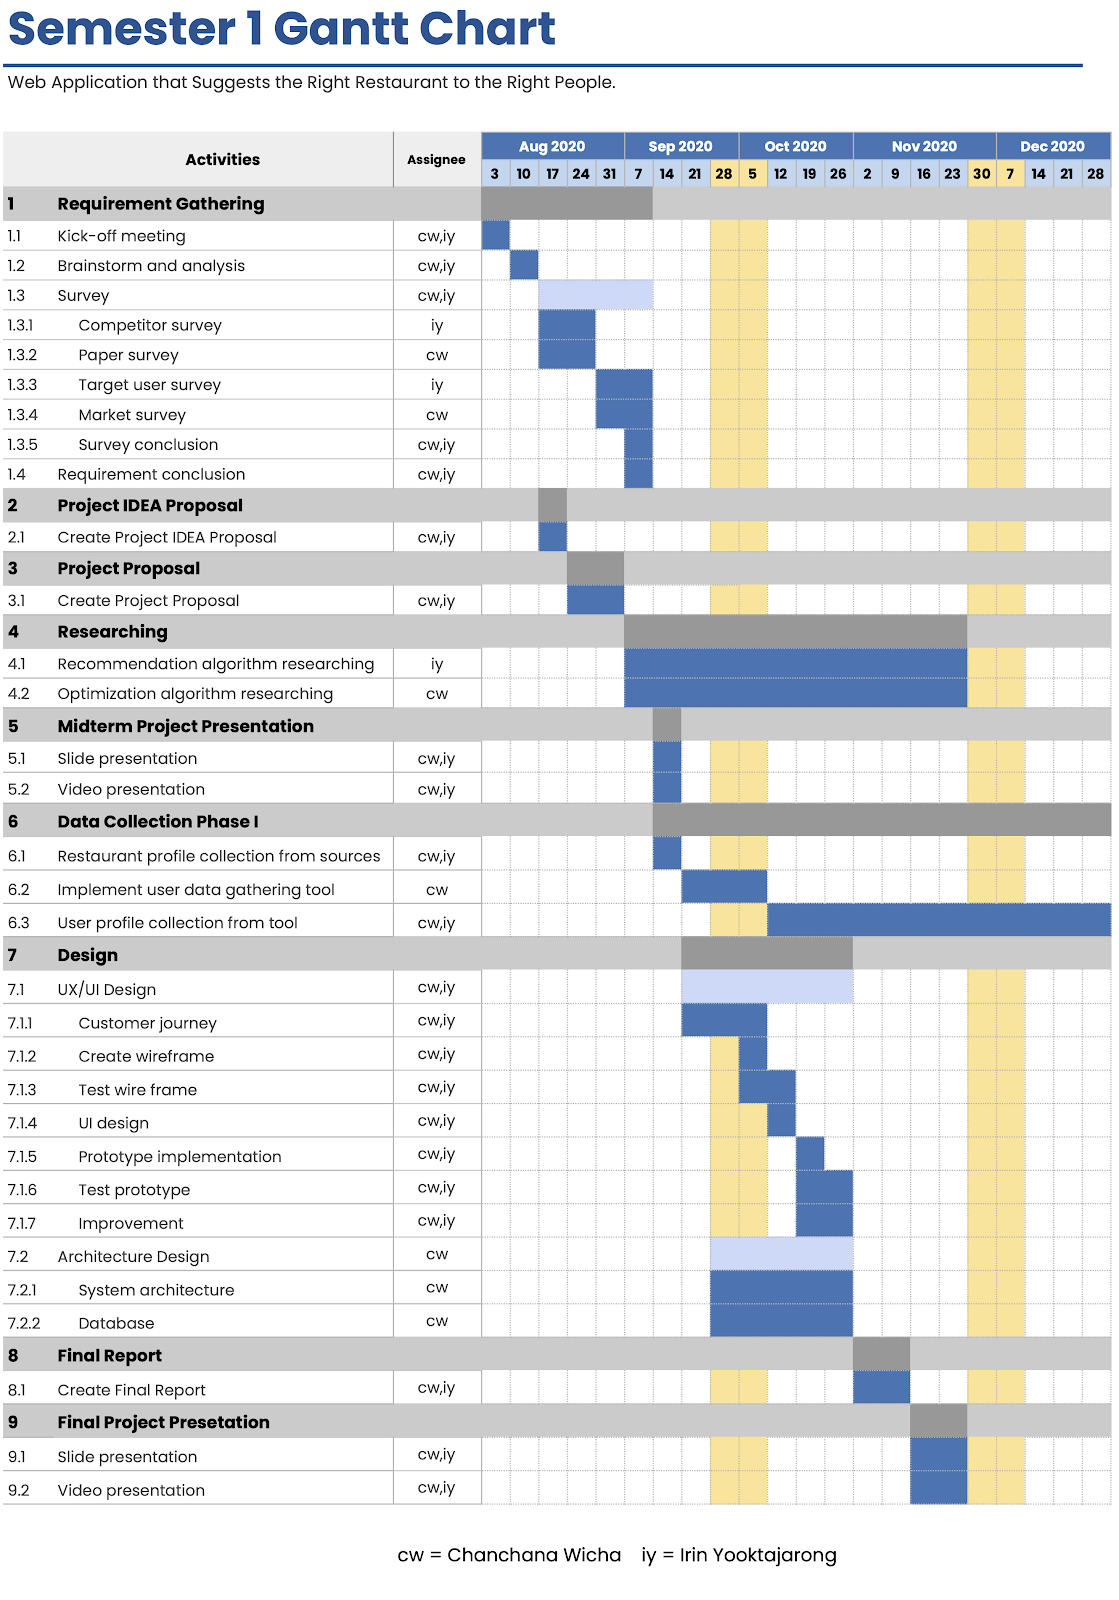
\includegraphics[width=440pt]{./images/1gantt1.png}
\caption{Gantt Chart for the First Semester}\label{fig:1_1}
\end{figure}\vspace{-24pt}

\begin{figure}[H]\centering
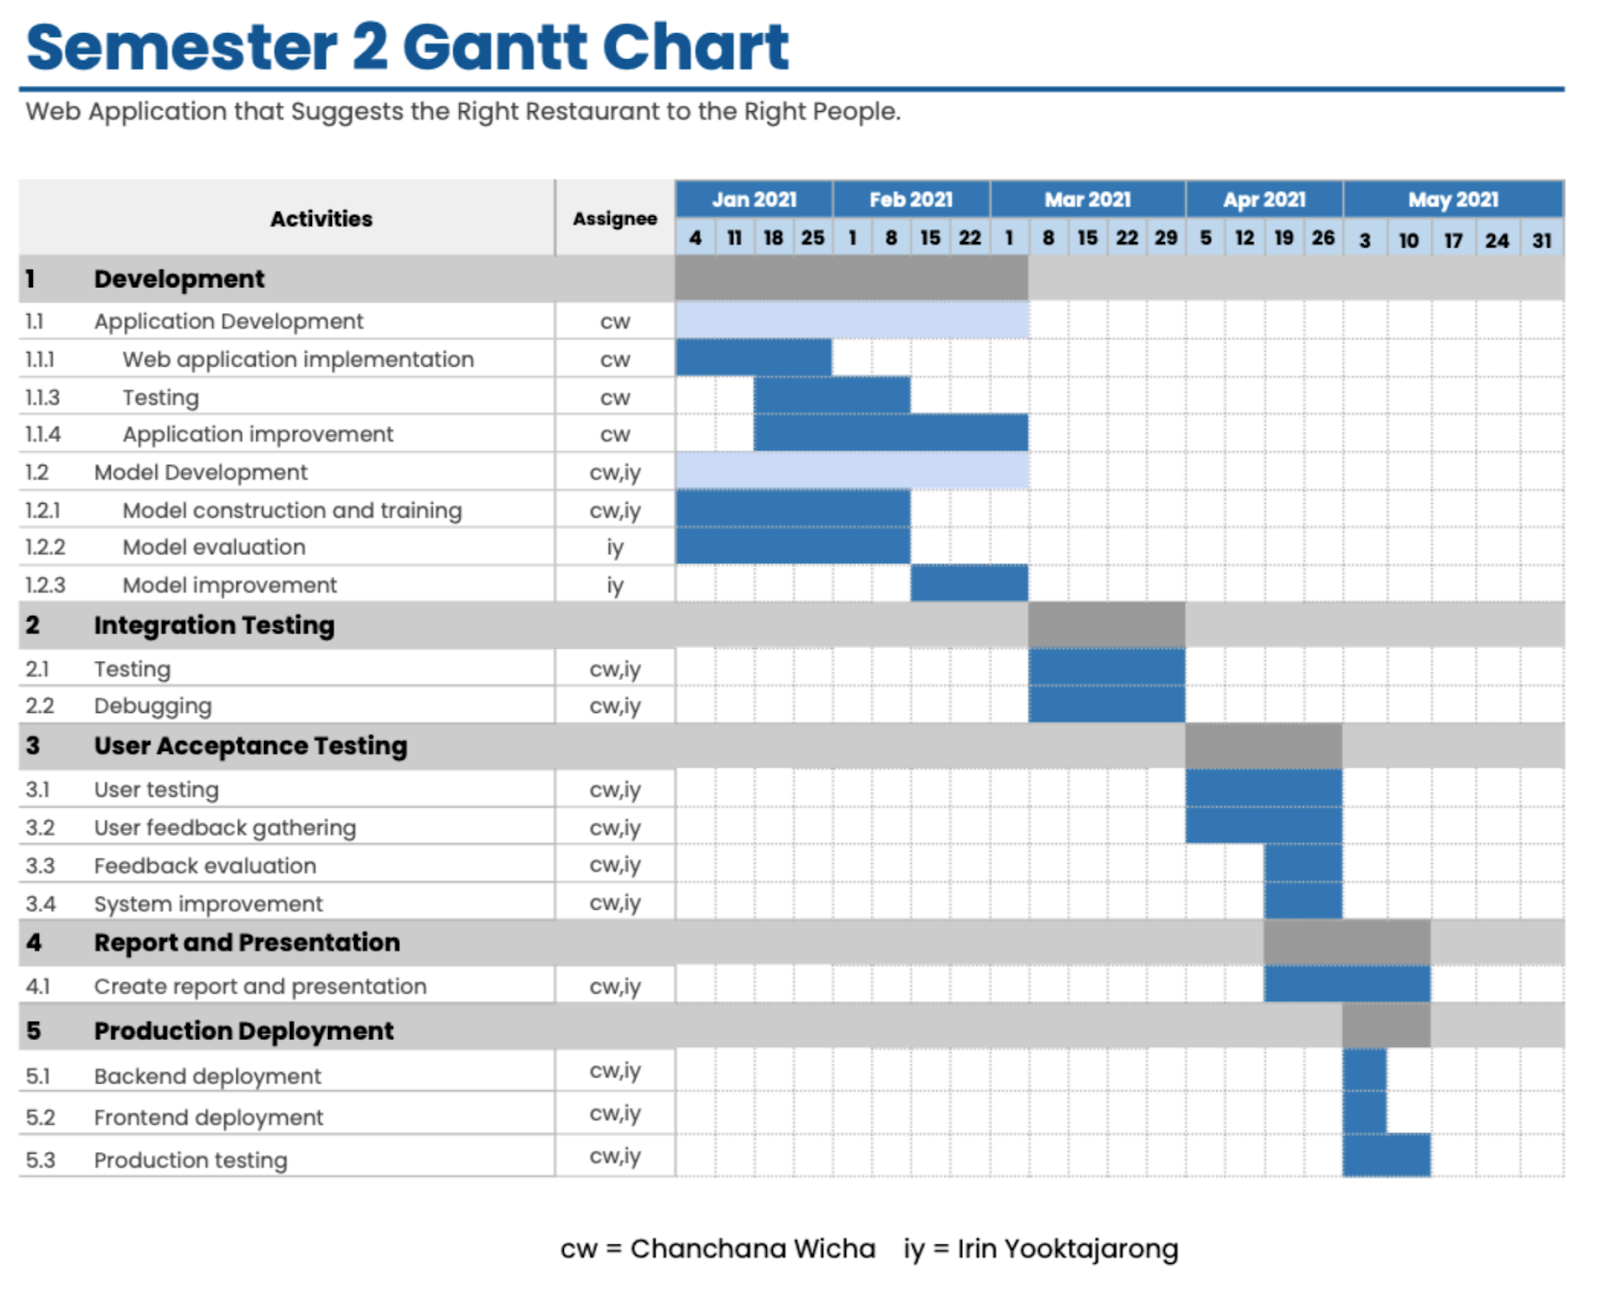
\includegraphics[width=440pt]{./images/1gantt2.png}
\caption{Gantt Chart for the Second Semester}\label{fig:1_2}
\end{figure}\vspace{-24pt}

\newpage

\section{Deliverables for Term 1} 
\begin{itemize}
\item Requirement Specification
\item Survey Result
\item Data Collection Tool
\item Dataset (Customer Behavior and Restaurant Information)
\item Customer Journey
\item Prototype (Web Application)
\item Database Schema
\item System Architecture and Class Diagram
\item Suggestion Algorithm and Model
\end{itemize}

\section{Deliverables for Term 2} 
\begin{itemize}
\item Web Application (Frontend and Backend)
\item Recommendation System both Individuals and Groups
\item Feedback from Users
\item Application Performance Evaluation
\item Model Performance Evaluation
\end{itemize}


%%%%%%%%%%%%%%%%%%%%%%%%%%%%%%%%%%%%%%%%%%%%%%%%%%%%%%%%%%%%
%%%%%%%%%%%%%%  Literature Review %%%%%%%%%%%%%%%%%%%%%%%%%%
%%%%%%%%%%%%%%%%%%%%%%%%%%%%%%%%%%%%%%%%%%%%%%%%%%%%%%%%%%%%
\chapter{Background Theory and Related Work}

\section{Background}

As the world becomes more digital and technology is all around us, before we realized it, we were accustomed to a personalized experience. Many online businesses are implementing personalized recommendation systems that try to identify a user’s preferences and provide them with relevant items to enhance the user's experience. However, mainstream restaurant recommendation applications in Thailand have not implemented personalized recommenders yet. This leads to the issue of finding an ideal restaurant which is always struggling for users and a person who is looking for new restaurants. Furthermore, the online problem survey revealed that many people faced a harder time to decide due to the group eating. Therefore, group decision making is very complex and time-consuming.

We brought this problem up to solve it since it is a common problem that everyone faces in daily life and no solution can be solved sustainably. Moreover, the majority of recommender systems are designed for individual users and the group recommender is challenging and new in the market. Inspired by such a challenge, we will invent a restaurant recommender system that could potentially reduce decision-making time for both individuals and groups and be an alternative way for users to opt for their ideal restaurants. Our system considers the interaction between users and restaurants and also uses side information e.g. users’ tastes and preferences, restaurant profile, etc. This approach is able to maximize users’ satisfaction and increase users’ experience.


\section{Related Theory}

\subsection{Web Application}

A web application is an application program that is stored on a remote server and delivered over the internet through a browser interface. \cite{WhatIsWebApplicationWebAppsAndItsBenefits} Because web applications are delivered through the internet, users do not need to install the application and it also allows multiple users access to the application at the same time on the same version. Moreover, running web applications require only an internet browser, so a web application is a platform and operating system independent.

Because our platform needs to be easily accessible for users not only individual users but also every member in the group of users, having a web application that does not require any installation and platform independence is a perfect solution. Users can easily access our platform via their mobile internet browser and all of them will see the same version of the application. A web application also accommodates the development process since we do not need to implement the different versions for different platforms.


\subsection{Information Collection}

This collects relevant information of users to generate a user profile or model for the prediction tasks including the user’s attributes, behaviors, or content of the resources the user accesses. \cite{WhatisMachineLearning} We need to do this process due to the recommender cannot provide results accurately until the users’ profile and preferences have been constructed. However, the information we collected includes username, password, and their users’ restaurant preference where all of them do not relate to personal information. So, PDPA or Personal Data Protection Act does not need to be concerned in our project.

There are several types of information/feedback that can be captured and studied including explicit and implicit feedback.

\subsubsection{Explicit Feedback}

The accuracy of the recommendation depends on the number of ratings provided by the user. The only shortcoming of this method is, it requires effort from the users and also, users are not always ready to supply enough information. Despite the fact that explicit feedback requires more effort from the user, it is still seen as providing more reliable data, since it does not involve extracting preferences from actions, and it also provides transparency into the recommendation process that results in a slightly higher perceived recommendation quality and more confidence in the recommendations. \cite{Recommendersystem}

\subsubsection{Implicit Feedback}

The system automatically infers the user’s preferences by monitoring the different actions of users such as the history of purchases, navigation history, and time spent on some web pages, links followed by the user, content of an email, and button clicks among others. Implicit feedback reduces the burden on users by inferring their user’s preferences from their behavior with the system. The method though does not require effort from the user, but it is less accurate. Also, it has been argued that implicit preference data might in actuality be more objective, as there is no bias arising from users responding in a socially desirable way. \cite{Recommendersystem}


\begin{table}[H]
\caption{Characteristics of Explicit and Implicit Feedback}\label{tbl:2CharacteristicsofExplicitandImplicitFeedback}
\begin{tabular}{l|l|l} \hline\hline
Implicit Feedback & Explicit Feedback & Accuracy \\ \hline\hline
Low & High & Abundance \\ \hline
High & Low & Context-sensitive \\ \hline
Yes & Yes & Expressivity of user preference \\ \hline
Positive & Positive and Negative & Measurement reference \\ \hline
Relative & Absolute \\ \hline\hline
\end{tabular}\par
\smallskip
Source: https://core.ac.uk/download/pdf/207051652.pdf
\end{table}


From Table~\ref{tbl:2CharacteristicsofExplicitandImplicitFeedback}, the accuracy of implicit feedback is lower than explicit feedback due to system monitoring only (indirect way). But with this approach, we can get abundant feedback whereas explicit feedback is scarce. Moreover, implicit feedback can capture only positive e.g. if a user never visits restaurant A that does not mean he/she does not like that restaurant. Although implicit feedback tends to be relative such as if a user visited restaurant B 10 times and restaurant C 100 times, then we can conclude that he/she has a higher preference for C than B. Lastly, as we can see from the table, one thing that is similar to each other is both are sensitive to the context

\subsection{Overview of Machine Learning}

Machine learning is an application of artificial intelligence (AI) that provides systems’ ability to automatically learn and improve from experience without being explicitly programmed. \cite{WhatisMachineLearning} Machine learning is often categorized into 3 types which are supervised learning, unsupervised learning, and reinforcement learning.

In supervised learning, it is learned from the labeled data and predicts the future events from the labeled e.g. classified cats and dogs. In contrast, unsupervised learning deals with unlabeled data which is extremely useful to discover patterns, not just predict the future from labeled data e.g. customer segmentation. Last is reinforcement learning which is the closest to human learning by learning to take corrective action with the provided environment, for example, AlphaGo which lets the machine learn how to play Go.

As our project is a recommendation system that needs to predict the next user-preferred restaurants from interactions and side information which mainly are unlabelled data. So, the model works on its own to discover patterns and information which is the restaurant for each user based on preferences. In addition, this project is an unsupervised learning problem.


\subsection{Recommendation System Techniques}

Recommender systems are usually as if a decision making strategy that helps users select the interest items based on users’ preferences or profile from overwhelmed available items or complex environments. There are 3 main types of recommendation filtering techniques which are content-based, collaborative, and hybrid. Each of these has different features and potentials.

\subsubsection{Content-based Filtering Technique}

Content-based filtering is a technique which recommends based on the similarity between the items and using users’ profile/description. Items that are mostly related to the positive user’s evaluation are recommended to the user. This approach uses a variety of models to find the similarity document to get meaningful suggestions by treating the recommendation as a user-specific classification problem by classifying for the user's likes and dislikes based on an item's features. \cite{Collaborativefiltering} Moreover, it does not require other users’ profiles as they do not affect recommendations, for example, the system wants to recommend the product which is similar to the product that user has purchased in the past, so they use content-based filtering to be the recommender by using the characteristics of the product to recommend including genre, price, style, description, picture, etc.

Therefore, this technique has the ability to recommend new items even if there is no user’s evaluation/rating. This would mean that it is able to recommend accurately without user preferences which consequence that if there is a poor description of items and an unorganized user profile, it can lead to the worst recommendation. So, the effectiveness of the content-based filtering technique depends on the richness of descriptive information, but lastly, it is unable to recommend a product that is very different from the product that the user previously purchased, resulting in the user receiving a not diverse category of product. To overcome this, it can adapt to some form of a hybrid system.

Moreover, from this approach, our project can use the algorithm to be part of our recommendation system which makes the system have an ability to recommend a restaurant even if there’s no user preference or we can say that we are able to overcome the new user problem.


\subsubsection{Collaborative Filtering Technique}

\begin{figure}[H]\centering
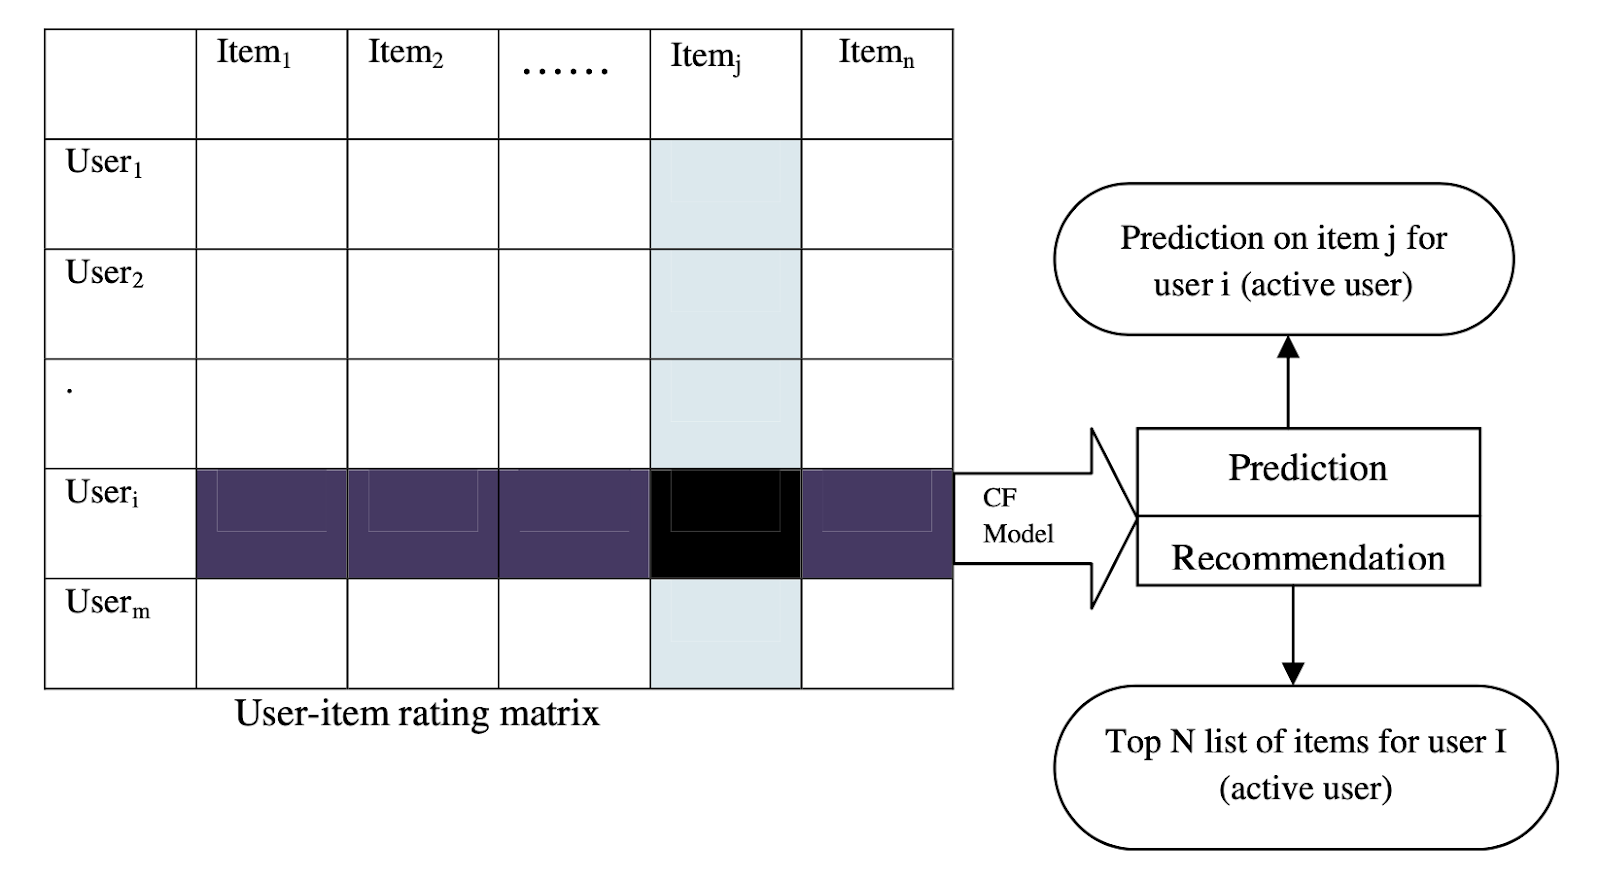
\includegraphics[width=250pt]{./images/2cfprocess.png}
\captionsource{Collaborative Filtering Process}{www.sciencedirect.com/science/article/pii/S1110866515000341}
\label{fig:2cfprocess}
\end{figure}\vspace{-24pt}
\vspace{1em}

A collaborative filtering technique as opposed to the content-based filtering technique which collaborative filtering cannot recommend the item by using only the description of metadata. The key idea of this technique is a group of people with similar tastes, often tend to like similar items. So, collaborative filtering uses only data about rating profiles from different users or items in order to generate the recommendation. Here is the flow of this technique:

\begin{enumerate}
\item Gather user expression from her/his preferences by items rated.
\item Match the user’s ratings with other users’ then find the most similar tastes.
\item Recommend with the high rating of unseen items from similar users to this user.
\end{enumerate}

To recommend, it works by creating a user-item matrix of preferences for items by users, as Figure~\ref{fig:2cfprocess} above which represents the process start from the matrix to the output of this system, and then calculating the similarity between profiles to get the relevant item that matches the user. Thus, the user will be able to get the items that he/she has not rated yet but already rated from a similar user. This approach can produce the output either prediction or recommendation by prediction represented as a score of an item for the user whereas recommendation is represented as a top N list of items as mentioned in Figure~\ref{fig:2cfprocess}. Collaborative filtering techniques can separate into 2 main categories: memory-based and model-based.


\textbf{1. Memory-based}\par

Memory-based can approach in 2 ways which are user-based and item-based.

User-based collaborative filtering is to find the users who are similar to the target user and then recommend by calculating the weighted averages of the ratings from the group of similar users. For item-based collaborative filtering is calculating the similarity between items instead of users for determining the items which are similar to the target item then, calculating the weighted average of the ratings from a group of similar items.

To calculate the weighted average, there are several popular similarity measurements to find the similarity between user/item including Pearson correlation coefficient and Cosine similarity.

\begin{equation}\label{eq:simil}
simil(x, y) = \frac{\sum_{i\in I_xy}^{}(r_{x,i}-\bar{r}_{x})(r_{y,i}-\bar{r}_{y})}
{\sqrt{\sum_{i\in I_xy}^{}(r_{x,i}-\bar{r}_{x})^2}\sqrt{\sum_{i\in I_xy}^{}(r_{y,i}-\bar{r}_{y})^2}}
\end{equation}

From the above example equation~\ref{eq:simil}, it is a Pearson correlation coefficient, $simil(x, y)$ denotes the similarity between 2 users $x$ and $y$, mean the rating given to the item $i$ by user $x$, $\bar{r}_{x}$ means the mean rating of user $x$, $I_{xy}$ and is equal to a total number of items in the user-item.


\begin{equation}\label{eq:cos}
cos(\vec{x},\vec{y}) 
=\frac{\vec{x}\cdot \vec{y}}{\left \| \vec{x} \right \|\times \left \| \vec{y} \right \|}
=\frac{\sum_{i\in I_xy}^{}r_{x,i}r_{y,i}}
{\sqrt{\sum_{i\in I_xy}^{}r_{x,i}^2}\sqrt{\sum_{i\in I_xy}^{}r_{y,i}^2}}
\end{equation}

For cosine similarity~\ref{eq:cos}, it is different from Pearson correlation coefficient which calculates as a vector-space model by measuring the similarity between dimensional vectors based on the angle which $cos(\vec{x},\vec{y})$ denotes to the similarity between 2 users $x$ and $y$.


\textbf{2. Model-based}\par

This approach is able to improve the performance of collaborative filtering by constructing the model which is done by using machine learning or data mining techniques. Moreover, with this approach, dimensionality reduction methods are mostly being used as complementary techniques to improve the robustness and accuracy of the memory-based approach. \cite{Recommendersystem}

For example, this technique is matrix factorization which is able to discover hidden concepts and their relationship with users and items.

\

The advantage of the collaborative filtering technique is performed in domains where there is not much content associated with items and where content is difficult for a computer system to analyze such as opinions and ideas. \cite{Recommendersystem} But there is some disadvantage which is about the cold-start problem which refers to the new user or item that comes with the empty profile since the user has not rated any item yet. Moreover, a memory-based approach has a problem with scalability. This issue can be solved by the model-based approach.

Collaborative filtering can perform better than content-based filtering in poor content. With the advantages of this technique, we are able to reduce the user effort by performing with the implicit feedback that comes from the system monitoring and get the recommendation result more accurately.


\subsubsection{Hybrid Filtering Technique}

The hybrid filtering technique is the most recommender system used nowadays. It is a combination of content-filtering, collaborative filtering, and other approaches. There are several ways to implement e.g. doing content filtering and collaborative filtering predictions separately and then combining them later, etc. Combining different recommendation techniques can provide a better system and be able to overcome the limitations of a pure recommendation system.

Therefore, the Hybrid approach can give a better recommendation than a pure approach and can avoid the cold-start problem, sparsity, scalability, and other problems.

According to both techniques which are content-based and collaborative filtering, we found that they can reduce both of their problems whether cold-start problems that come from collaborative filtering which are content-based able to overcome, or about the diversity recommendation problem which hybrid approach can overcome. In our opinion, the hybrid filtering technique is the best choice to be done in a restaurant recommendation system.
        
        

\subsection{Aggregation Mechanism}

Since this project aims to recommend the restaurant to users both individuals and groups, we need to aggregate individual preferences into group preferences before recommending restaurants to a group of users. There are many existing strategies for aggregation but the key idea of this approach is how the individual group members’ preferences are combined into a group preference.

For the aggregating preferences strategy, the individual preferences will be aggregated into groups by combining the user’s preferences/ratings of each item and let this be the group rating. Then, group recommendations will be based on this preference and offer only the top N recommendations list to the group which N refers to the number of items that will be recommended to a group.

\subsection{Optimization Techniques}

The optimization algorithm is a procedure which is executed iteratively by comparing various solutions till an optimum or a satisfactory solution is found \cite{AlgorithmsforDiscreteOptimization} which can be either the minimum or the maximum value. The optimal value can be selected from a set of available solutions with some criterion \cite{Mathematicaloptimization}. Examples of objective functions that require maximum values ​​are: number of kilometers that a delivery vehicle can run per 1 gallon of fuel, number of customers, number of customers eating in a restaurant per hour, etc. Examples of objective functions that require minimum values ​​are: cost per unit of production, factory electricity consumption per hour, and so on.

In this project, we have adopted a method of optimization to define the objective function of our system. The objective of our system is to maximize the satisfaction of users based on the recommendations of restaurants that meet the interests and needs of that user.

\subsection{Genetic Algorithm}

The genetic algorithm (GA) is a metaheuristic method inspired by the process of natural selection that belongs to the larger class of evolutionary algorithms (EA). Genetic algorithms are commonly used to generate high-quality solutions to optimization and search problems by relying on biologically inspired operators such as mutation, crossover, and selection. \cite{Geneticalgorithm}

In the genetic algorithm, the optimal solution is found by replacing an existing set of parameters in the form of chromosomes. Each parameter in the chromosome is known as a gene which is usually replaced with numbers by encoding methods.  The first step in solving a problem is chromosome encoding, which varies depending on the problem. The initial population will be random values. To find the fitness solution, each generation will either mutate or switch genes between each other until a new generation of population with more fitness is obtained, this evolving process will continue until a suitable answer is found. The overall process of genetic algorithms is shown in the following pseudocode.

%TODO use algorithm package

\textbf{Genetic Algorithm Pseudocode}\cite{IntroductiontoGeneticAlgorithmsIncludingExampleCode}\\
\textbf{1} START\\
\textbf{2} Generate the initial population\\
\textbf{3} Compute fitness\\
\textbf{4} REPEAT\\
\textbf{5} \quad Parent Selection\\
\textbf{6} \quad Crossover/Mutation\\
\textbf{7} \quad Compute fitness\\
\textbf{8} UNTIL population has converged\\
\textbf{9} STOP\\

The genetic algorithm consists of 4 main phases: Initial Population, Selection, Reproduction, and Termination. The details of each phase are as follows.


\paragraph*{1. Initial Population}\

A population is made up of chromosomes. Each chromosome, which is a set of genes, represents a solution to a problem that needs to be solved. The chromosome encoding process must start at the beginning. The dimensions of a problem solution must be encoded in a string of genes using some encoding techniques. The most popular approach is binary encoding, which defines the solution as sequences of 1s and 0s. Then, the value of genes is randomized.

\paragraph*{2. Selection}\

The idea of selection is to select the appropriate chromosomes or the fitter chromosomes measured by a fitness function and pass them to the next generation to be able to get a more optimal answer to the problem. Generally, chromosomes with higher fitness have more chances than lower fitness to reproduce.

\paragraph*{3. Reproduction}\

After the selection process, this process will use those chromosomes to generate the next generation by either crossover or mutation. Crossover is the most significant phase in a genetic algorithm. For each pair of parents to be mated, a crossover point is chosen at random from within the genes. \cite{IntroductiontoGeneticAlgorithmsIncludingExampleCode} After that, offspring will be created and added to the population of next generation. For mutation, it occurs when new offspring are formed by flipped some bits. This process exists to maintain the diversity of population and prevent premature convergence.

\paragraph*{4. Termination}\cite{Geneticalgorithm}

This generational process is repeated until a termination condition has been reached. Common terminating conditions are:

\begin{itemize}
\item A solution is found that satisfies minimum criteria
\item Fixed number of generations reached
\item Allocated budget (computation time/money) reached
\item The highest ranking solution's fitness is reaching or has reached a plateau such that successive iterations no longer produce better results
\item Manual inspection
\item Combinations of the above
\end{itemize}

\

In this approach, we can create a recommendation system for both individuals and groups which is based on users’ preferences along with the user's restaurant selection history. Genetic algorithms approach is the most likely to be able to serve our objective which is to maximize the satisfaction of users.




\section{Technologies}

\subsection{Development Tools}

\subsubsection{HTML}

HTML (HyperText Markup Language) is the most basic building block of the Web. It defines the meaning and structure of web content. HTML uses "markup" to annotate text, images, and other content for display in a Web browser. HTML markup includes special "elements" such as <body>, <p>, <div> and many others. An HTML element is set off from other text in a document by "tags", which consist of the element name surrounded by "<" and ">". \cite{HTMLHyperTextMarkupLanguage}

\subsubsection{JavaScript}

MDN \cite{JavaScript} states that JavaScript is a programming language that enables complex feature implementation on web pages such as displaying timely content updates, interactive maps, animated 2D/3D graphics, scrolling video jukeboxes, etc. Many modern browsers such as Google Chrome, Safari, and Firefox support JavaScript and it can run immediately within the browsers without repeatedly calling the server.

JavaScript is able to implement those complex features described above because it supports the use of the Document Object Model (DOM), a collection of APIs for controlling HTML and styling details \cite{Manipulatingdocuments}. With DOM, we can easily write JavaScript to modify HTML elements interactively.
Because our platform needs to serve an interactive user interface with a fast speed, these characteristics and advantages of JavaScript can fulfill those requirements. However, there are limitations of JavaScript. The first limitation is that it lacks the feature of reading and writing local files for security reasons, which needs the use of another server-side service to handle more complex tasks. The other limitation is that different browsers can sometimes interpret JavaScript code differently. However, since we aim to support most of the modern browsers, we do not have to worry about this limitation.

\subsubsection{TypeScript}

TypeScript extends JavaScript by adding types. By understanding JavaScript, TypeScript saves us time catching errors and providing fixes before we run code. \cite{TypeScript} The reason that we choose TypeScript over plain JavaScript is it makes our platform easily maintainable by adding static types and error checking.

\subsubsection{Node.js}

Node.js is an open-source and cross-platform JavaScript runtime environment. \cite{IntroductiontoNodejs} Because we choose to have a JavaScript web application framework, Node.js is essential for running our scripts. In the server side services, Node.js is the environment that runs the application and actively serves the clients request, while in the client side services, Node.js may be used to build the optimized bundled package that serves the client.

\subsubsection{React}

React is a library for building composable user interfaces. It encourages the creation of reusable UI components which present data that changes over time. \cite{WhydidwebuildReact} The DA14 blog \cite{TOP10ADVANTAGESOFUSINGREACTJS} demonstrates the top 10 advantages of React including JSX syntax and reusable components. The first advantage, React uses JSX syntax which is an extension syntax to JavaScript. It makes subcomponent rendering easier by accepting HTML quoting, thus the overall process of writing components is much simpler. The other one of their best features is an ability to reuse components which makes a codebase more clean and easy to maintain. In our project, we want our development process to be simple and our codebase to be clean and maintainable, so React is the perfect solution. Moreover, React supports TypeScript that adds the static type to our JavaScript which also facilitates our development process.

\subsubsection{Python}

Python is a general-purpose interpreted, interactive, object-oriented, and high-level programming language. \cite{PythonTutorial} According to PYPL PopularitY in November 2020, Python is the most popular programming language. Due to its popularity, Python has hundreds of different libraries and frameworks which is a great addition to your development process. \cite{Top7ReasonsWhyYouNeedtoLearnPythonasaDataScientist} Many of these libraries and frameworks are mainly focused on data analytics and machine learning. Examples of those libraries are Numpy, Pandas, and Matplotlib. Our platform not only focuses on user experience but also data analytic and machine learning, so using Python fits perfectly in those areas.

\subsubsection{JupyterLab}

JupyterLab enables you to work with documents and activities such as Jupyter notebooks, text editors, terminals, and custom components in a flexible, integrated, and extensible manner. \cite{JupyterLabOverview} It is flexible and easy to arrange multiple notebooks or documents by showing in the tabs pattern. So, to do the experiment and construct the model of a recommendation system whether individuals or groups approach, this platform can provide a suitable working area to us. Moreover, JupyterLab also supports a variety of data formats e.g. images, CSV, JSON, etc.

\subsubsection{Figma}

Figma is a cloud-based design and prototyping tool for digital projects. It’s made so that users can collaborate on projects and work pretty much anywhere. \cite{WhatIsFigmaa101Intro} We choose Figma because of their collaborative feature which allows us to work together easily. Figma also allows us to test our prototype by sharing an online link to our testers.


\subsection{HTTP}

HTTP is a protocol that allows the fetching of resources, such as HTML documents. It is the foundation of any data exchange on the Web and it is a client-server protocol, which means requests are initiated by the recipient, usually the Web browser. \cite{AnoverviewofHTTP}

\begin{figure}[H]\centering
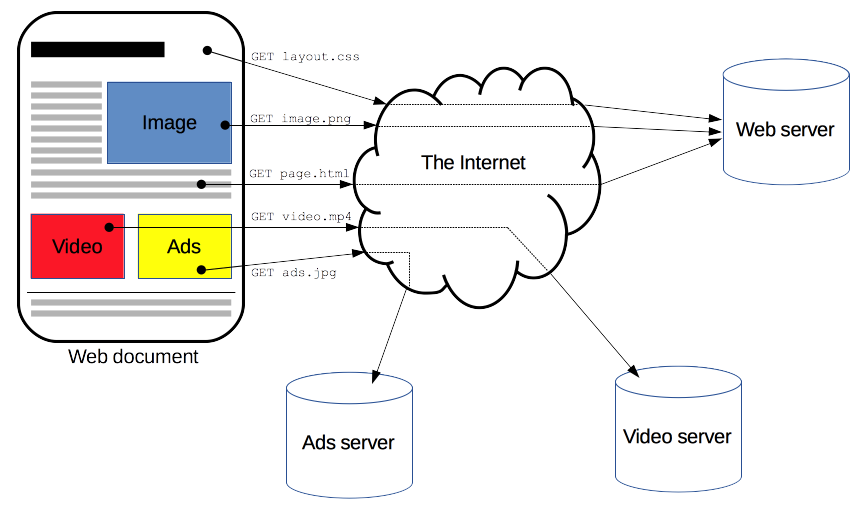
\includegraphics[width=250pt]{./images/2http.png}
\captionsource{Communication Through an HTTP Protocol}{https://developer.mozilla.org/en-US/docs/Web/HTTP/Overview}
\label{fig:2http}
\end{figure}\vspace{-24pt}
\vspace{1em}

Figure~\ref{fig:2http} shows how messages are communicated via the HTTP protocol. As you can see clients and servers communicate by exchanging individual messages. \cite{AnoverviewofHTTP} The messages sent from clients are requests. and the reply messages from servers are called responses.

HTTP defines a set of request methods for requests to indicate the desired action to be performed for a given resource. Although they can also be nouns, these request methods are sometimes referred to as HTTP verbs. \cite{HTTPrequestmethods} The common HTTP verbs are shown in Table~\ref{tbl:2CommonHTTPVerbs}.

\begin{table}[H]
\caption{Common HTTP Verbs}\label{tbl:2CommonHTTPVerbs}
\begin{tabularx}{\textwidth}{l|l} \hline\hline
Verb & Description \\ \hline\hline
GET & Retrieve data. \\ \hline
POST & Create data \\ \hline
PUT & Update data. \\ \hline
DELETE & Remove Data \\ \hline\hline
\end{tabularx}
\end{table}

%TODO check for update
One of the HTTP characteristics is HTTP is a stateless protocol in which no session information is retained by the receiver or server. Relevant session data is sent to the server by the client in such a way that every request sent can be understood in isolation, without context information from previous requests in the session. \cite{Statelessprotocol} To make servers manage and understand the session, we need to make use of Cookies which is compact-sized information sent with requests. The servers can use that information to identify the current session from every isolated request such as authentication which makes them understand who is sending the request and do not require users to login every time they need to interact with the system.


\subsection{Web Application Framework}

A web application framework is a software framework that includes a code library that makes web development quicker and easier by giving basic patterns for building reliable, scalable and maintainable web applications \cite{WhatIsWebFramework} so that we do not need to implement everything from the ground up. It can facilitate various functionalities for web development such as request handling, URL routing, transferring data phrasing and database connection configuration.

In our project, we choose Express framework for JavaScript with Node.js and Flask framework for Python. Both of them have a suitable functionality for our system with a large community base.

\subsubsection{Express}

Express is a minimal and flexible Node.js web application framework that provides a robust set of features for web and mobile applications. \cite{Express} The main advantages of Express are scalability and the language. Express lets us scale our application easily because of the support of Node.js and its lightweight. Express also uses JavaScript with TypeScript support, so we do not need to learn another programming language as we considered using TypeScript for frontend development.

\subsubsection{Flask}

Flask is a lightweight web application framework for Python. It is designed to make getting started quick and easy, with the ability to scale up to complex applications. \cite{Flask} Unlike full-stack web application frameworks such as Django, Flask offers only essential features for building a core web application, thus the performance is better and we can keep our codebase clean and simple. We need Flask in addition to Express because our project also focuses on data analytics and machine learning which also need communication to other components and implemented with Python, so Flask can seamlessly serve us those purposes.

\subsection{Database Tools}

\subsubsection{NoSQL}

NoSQL databases are non-tabular and store data differently than relational tables. They provide flexible schemas and scale easily with large amounts of data and high user loads. NoSQL databases come in a variety of types based on their data model. The main types are document, key-value, wide-column, and graph. \cite{WhatisNoSQL} The description of each type is shown in Table~\ref{tbl:2NoSQLTypesandDescription}.

\begin{table}[H]
\caption{NoSQL Types and Description}\label{tbl:2NoSQLTypesandDescription}
\begin{tabularx}{\textwidth}{l|X} \hline\hline
Type & Description \\ \hline\hline
Document & Store data in JSON-like objects, each field will have a key-value pair. Values in each field can have various types so that document-based NoSQL can be used as a general-purpose database. It also supports horizontal scaling to support a large volume of data. \\ \hline
Key-value & Key-value based NoSQL is simpler than document-based NoSQL because it contains one key and value. It is used for a large amount of data but not for a complex query. \\ \hline
Wide-column & Store each row of data in dynamic columns. It is suitable for data that we can predict the query pattern. \\ \hline
Graph & Store data in nodes and edges. Nodes generally store information while edges store their relation to other nodes. \\ \hline\hline
\end{tabularx}
\end{table}

According to Table~\ref{tbl:2NoSQLTypesandDescription}, the advantages of NoSQL which is flexible schemas and document-based NoSQL type which support complex query and horizontal scalability, we can conclude that document-based NoSQL is suitable to be our database tool because our data’s schema can easily change over time, we have a large amount of data and we need a complex query method for retrieving the data such as query objects sorted by distance from a coordinate.

\subsubsection{MongoDB}

%TODO check for update
MongoDB is a document-based NoSQL database used for high volume data storage. Instead of using tables and rows as in the traditional relational databases, MongoDB makes use of collections and documents. Documents consist of key-value pairs which are the basic unit of data in MongoDB. Collections contain sets of documents and functions which are the equivalent of relational database tables. \cite{WhatisMongoDBIntroductionArchitectureFeaturesExample} We choose to use MongoDB because it is open-source software, large community based, powerful query language and natively support database cloud service. We consider using their native cloud platform, MongoDB Atlas, which will be described later, so that we do not have to deploy our own database service by ourselves and the server side services can easily connect to the database with a simpler configuration.

\subsubsection{Mongoose}

Mongoose is a JavaScript library which provides a straight-forward, schema-based solution to model your application data. It includes built-in type casting, validation, query building, business logic hooks, and more, out of the box. \cite{mongoose} It also provides an interface to connect to the database. Although NoSQL does not have a fixed schema, having a schema for some essential fields in the model helps in a uniform data format that facilitates database operations in our system. Mongoose provides essential types for declaring the model’s schema. The essential types are shown and described in Table~\ref{tbl:2MongooseSchemaTypes} below.

\begin{table}[H]
\caption{Mongoose’ Schema Types}\label{tbl:2MongooseSchemaTypes}
\begin{tabularx}{\textwidth}{l|X} \hline\hline
Type & Description \\ \hline\hline
ObjectId & A special type typically used for unique identifiers \\ \hline
String & A sequence of characters in string format \\ \hline
Number & A real number which includes all types of number such as integer, float, or double. \\ \hline
Boolean & True or false state \\ \hline
Date & Datetime format \\ \hline
Object & Nested object \\ \hline\hline
\end{tabularx}
\end{table}


\subsection{Deployment Tools}

\subsubsection{Google Cloud App Engine}

Google Cloud App Engine is a fully managed, serverless platform for developing and hosting web applications at scale. It lets you choose from several popular languages, libraries, and frameworks to develop your apps, then let Google Cloud App Engine take care of provisioning servers and scaling your app instances based on demand. \cite{GoogleAppEngineDocumentation} Google Cloud App Engine is suitable for our platform which has 2 primary programming languages. It makes the deployment process much more simple.

\subsubsection{MongoDB Atlas}

MongoDB Atlas is a fully-managed cloud database developed by the same people that build MongoDB. Atlas handles all the complexity of deploying, managing, and healing your deployments on the cloud service provider. \cite{MongoDBAtlas} MongoDB Atlas is the perfect choice for us because it gives us life-time free 500 MB of storage space and all of the advantages of NoSQL stated before.


\subsection{External Service}

\subsubsection{Facebook Graph API}

%TODO check for update
Facebook Graph API is the primary way for apps to read and write to the Facebook social graph \cite{GraphAPI}. It provides a place query that we use for collecting restaurant data. Their restaurant information data includes restaurant tags which can help us in data analytics and machine learning process. We will write a script to query restaurant information from their API. Their API is free to use with the authentication token. The token is acquired by setting up the application on their platform.

\subsubsection{Google Cloud Storage}

Google Cloud Storage is a web service that allows storing and accessing data on a cloud. It provides a uniform process to access the static data. In our project, we need to keep the image of the restaurants and the total size of the images is too large to serve via our main server, Google Cloud Storage is the solution for this problem. Unlike Google Drive, Google Cloud Storage can set the static path for every restaurant image, but Google Drive will generate a random url to access the data. Another cloud storage service is Amazon S3, however, since we use Google Cloud Platform service which is Google Cloud App Engine for the deployment, Google Cloud Storage is a better choice for this project.


\section{Related Research/Competing Solutions}

\subsection{Entrée}

\begin{figure}[H]\centering
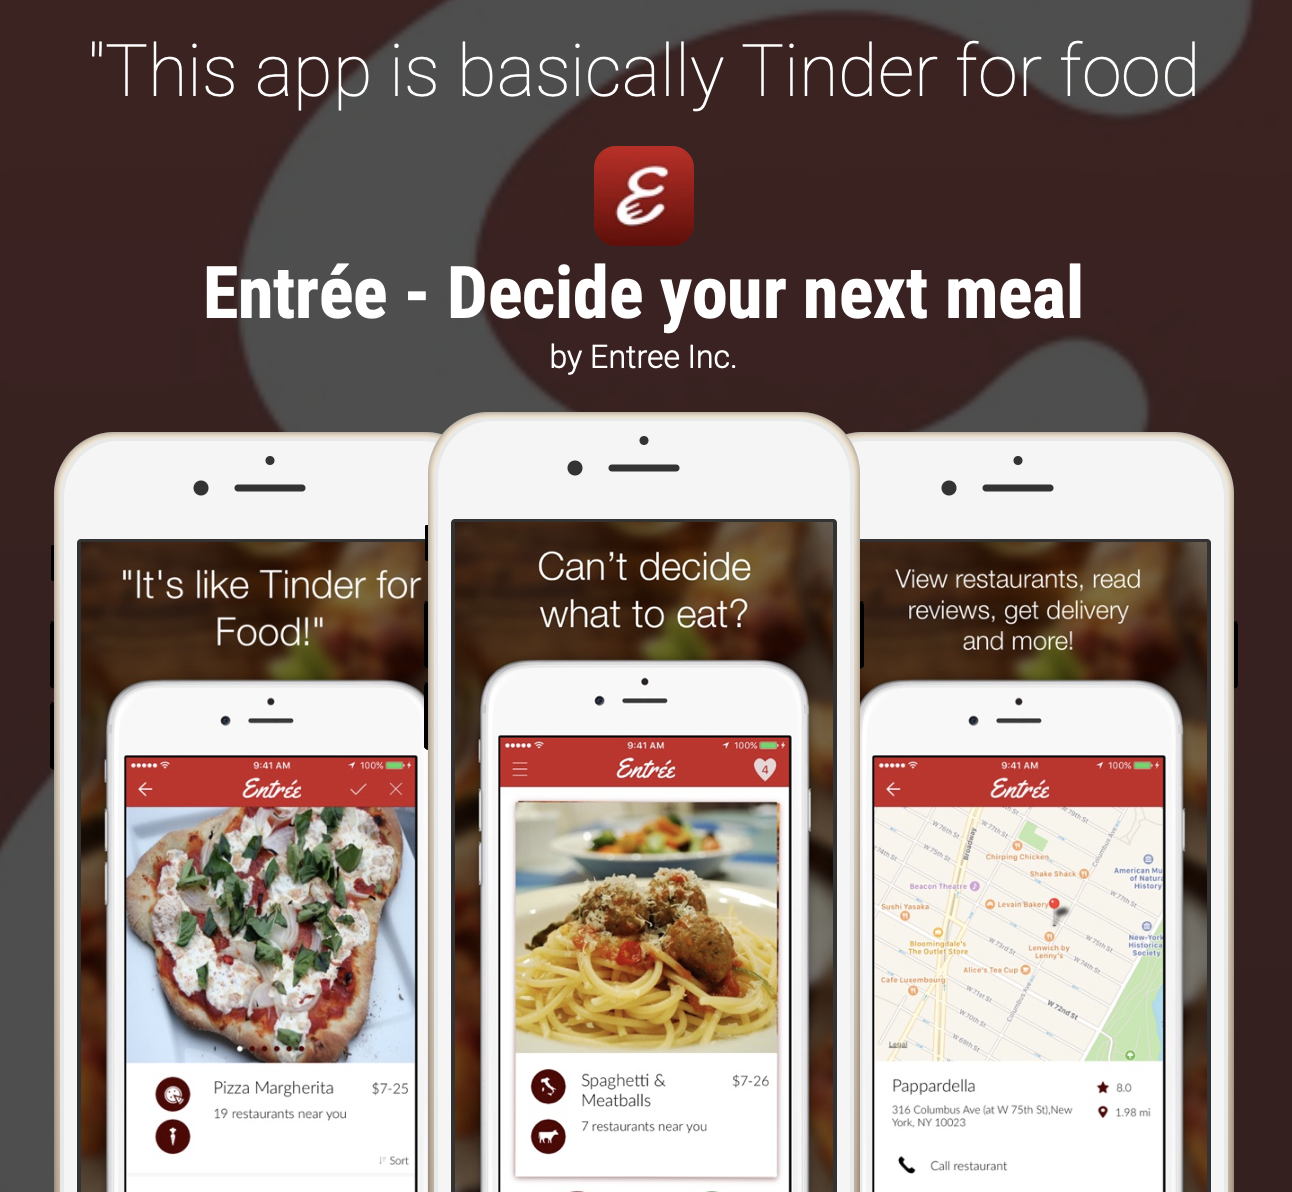
\includegraphics[width=400pt]{./images/2eatsee.png}
\label{fig:2eatsee}
\captionsource{Screenshot of Entrée Application}{https://appadvice.com/app/entr-c3-a9e-decide-your-next-meal/1037913795}
\end{figure}\vspace{-24pt}
\vspace{1em}

Entrée aims to solve the endless problem about what to order every day, by acting as a sort of “Tinder meets Pandora” for food. The app, freely available for download on iOS, shows users high-quality images of food or meals from nearby restaurants, based on an algorithm that learns users’ preferences. It also provides contextual recommendations, based on the occasion the user is looking to eat out for, like birthdays or date nights. The app is functional in 30 cities, and in the cities where Uber is also available, it allows users to book an Uber to the restaurant, call the restaurant and place your order for delivery. The app utilizes data from Foursquare for reviews and other information. \cite{Entréechoosefromaworldofdisheswithasingletouch}

Compared to our system, Entrée can suggest restaurants for only individuals, in contrast, our system support group suggestion. It supports 30 cities outside Thailand but our system has restaurants that are located in Thailand which uses Thai restaurant databases such as Wongnai and Google Places.

\newpage
\subsection{Eatsee}

\begin{figure}[H]\centering
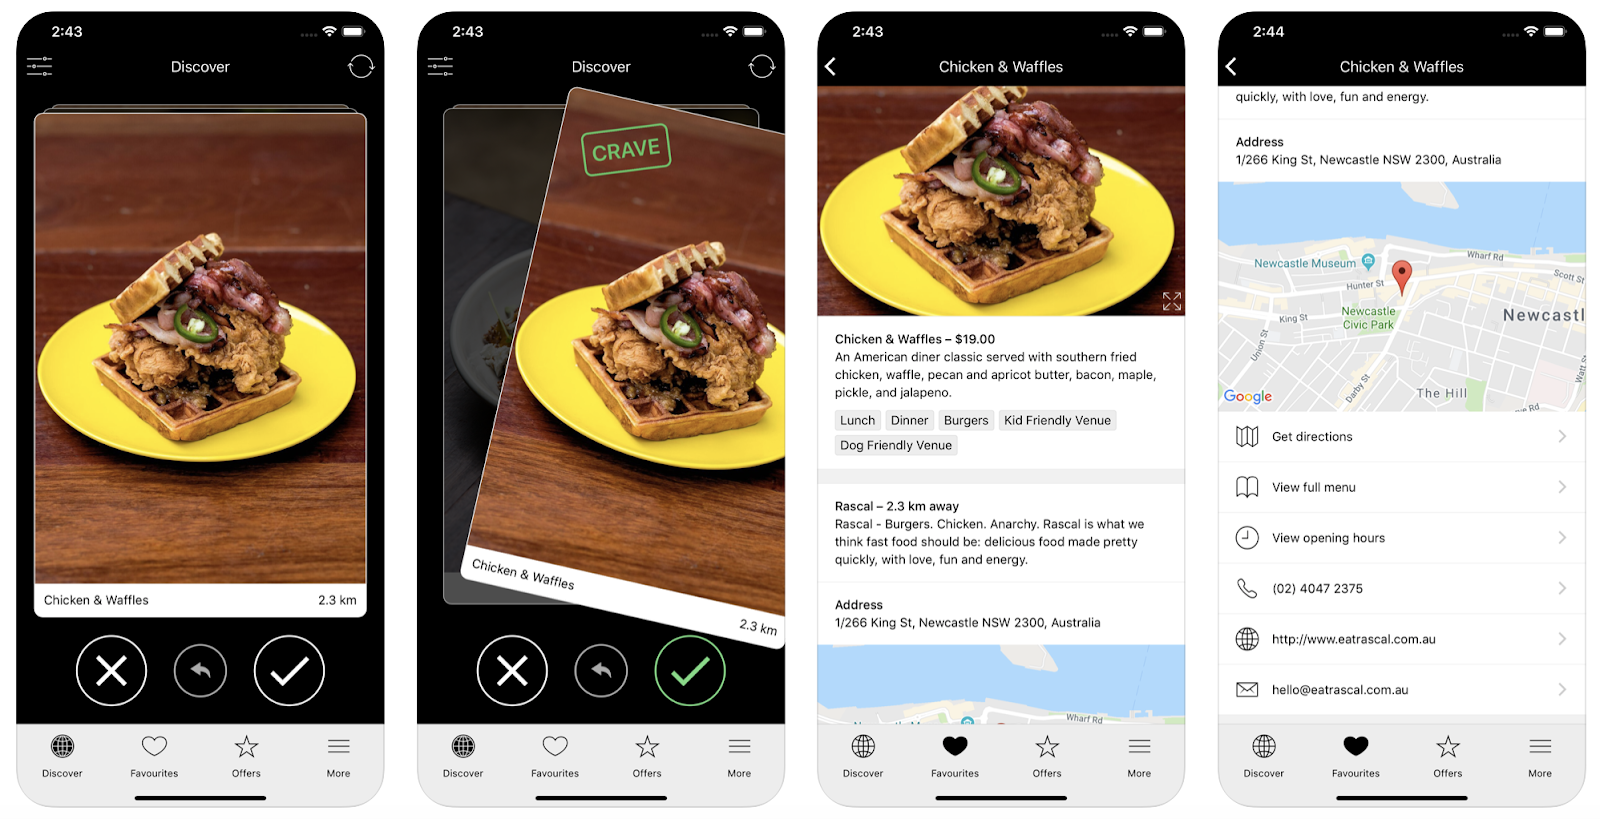
\includegraphics[width=400pt]{./images/2eatseereal.png}
\label{fig:2eatseereal}
\captionsource{Screenshot of Eatsee Application}{https://apps.apple.com/us/app/id1202110881}
\end{figure}\vspace{-24pt}
\vspace{1em}

Eatsee is an application that helps users find dishes that they’ll love by setting their preferences and swipe through user-tailored results, tap to find out more about the restaurant, then swipe right to save it to be favorites. Eatsee is currently available in Newcastle (New South Wales, Australia), Coffs Harbour (New South Wales, Australia), and San Francisco (California, United States). \cite{EatseeSeeitEatit}

Compared to our system, Eastsee only suggests random food based on their preference setting which doesn’t learn about users’ behavior. It focuses on food, not restaurants but our system prioritizes restaurants over food. It doesn’t support group suggestions and restaurants located in Thailand.
2whatman

\newpage
\subsection{Whatever Mans}

\begin{figure}[H]\centering
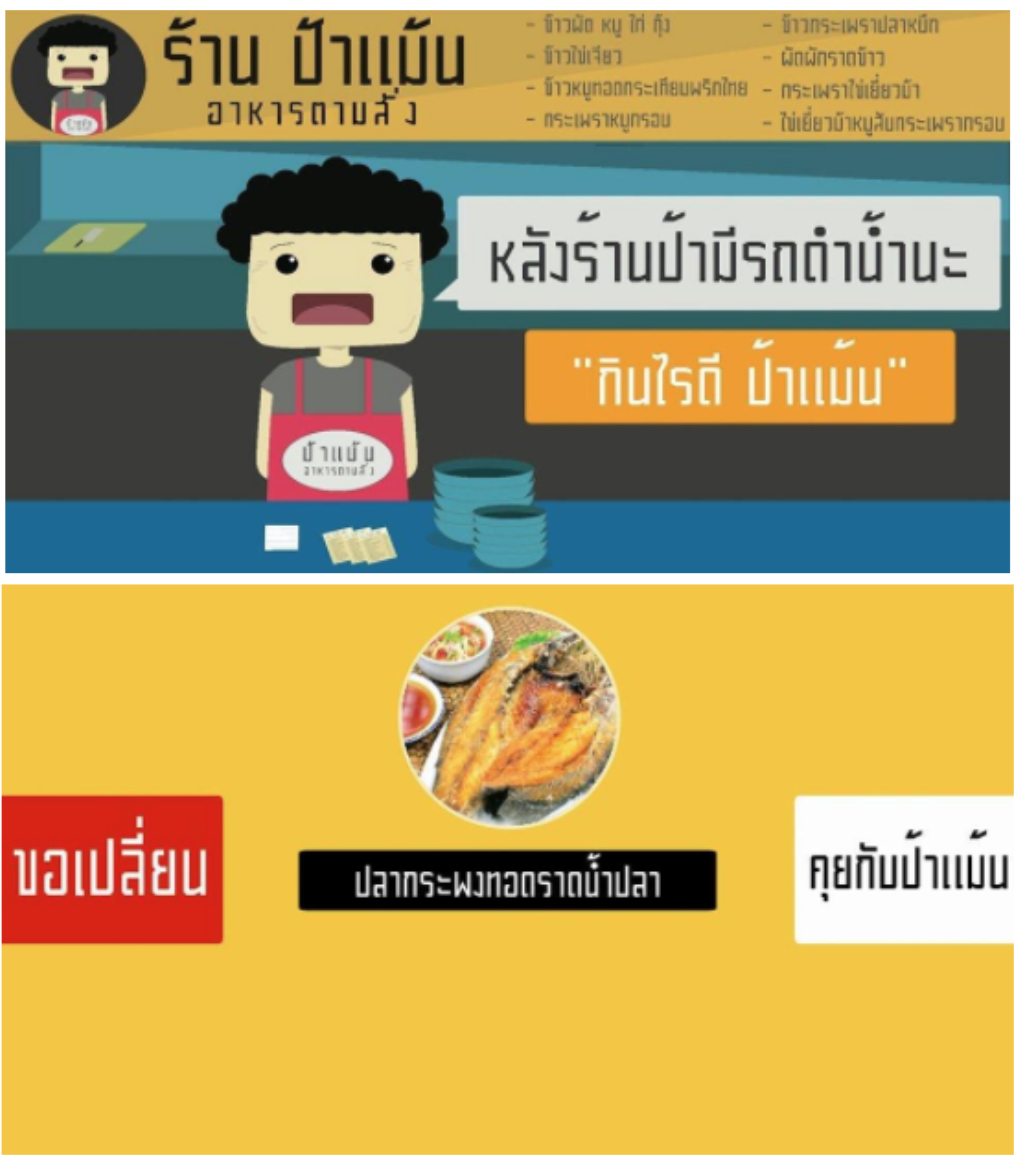
\includegraphics[width=250pt]{./images/2whatman.png}
\label{fig:2whatman}
\captionsource{Screenshot of Whatever Mans Application}{https://play.google.com/store/apps/details?id=com.DEC.Eatwhat}
\end{figure}\vspace{-24pt}
\vspace{1em}

Whatever Mans Application  ({\thaifont เที่ยงนี้กินไรดี}) is a Thai food random application that has an interaction with the user by creating an interactive animation called Pa-Man ({\thaifont ป้าแม้น}) to talk with the user. \cite{Whatevermans} Whatever Mans is available for download on Android only.

Compared to our system, Whatever Mans Application supports only on an Android platform whereas our system supports both iOS and Android because of web application technology. Their suggestion isn't based on users’ profiles or preferences which means their suggestion is just randomization. Although it supports Thai food, it can suggest only food, not restaurants. It also doesn’t support group suggestions.

\newpage
\subsection{Tinder}

\begin{figure}[H]\centering
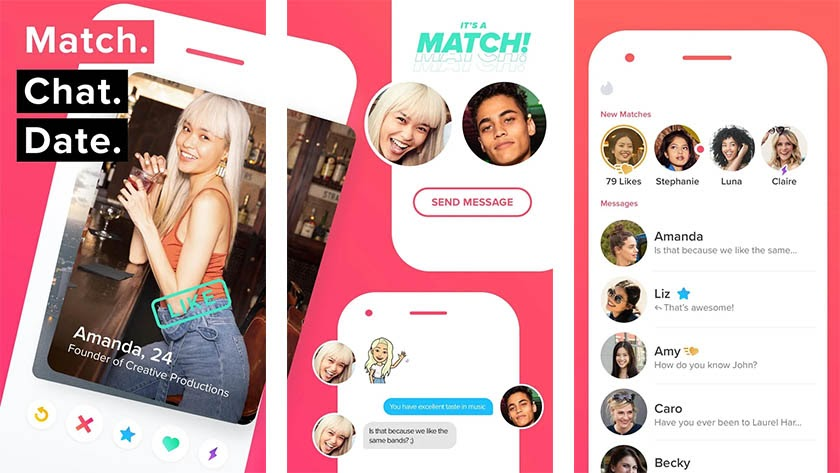
\includegraphics[width=400pt]{./images/2tinder.jpeg}
\label{fig:2tinder}
\captionsource{Screenshot of Tinder Application}{https://www.androidauthority.com/best-tinder-alternatives-android-1084559/}
\end{figure}\vspace{-24pt}
\vspace{1em}

Tinder is a geosocial networking and online dating application that allows users to anonymously swipe to like or dislike other profiles based on their photos, a small bio, and common interests. Once two users have "matched", they can exchange messages. \cite{Tinderapp}

Compared to our system, Tinder shares a similarity with our system which is a recommendation algorithm. It learns user preferences over time and suggests new people based on their preferences. However, their suggestion is based on individuals because it is a dating application.  The main contrast to our system is that Tinder focuses on suggesting new people whereas our system suggests restaurants.

\newpage
\subsection{On the design of Individual and Group Recommender Systems for Tourism Paper}

\begin{figure}[H]\centering
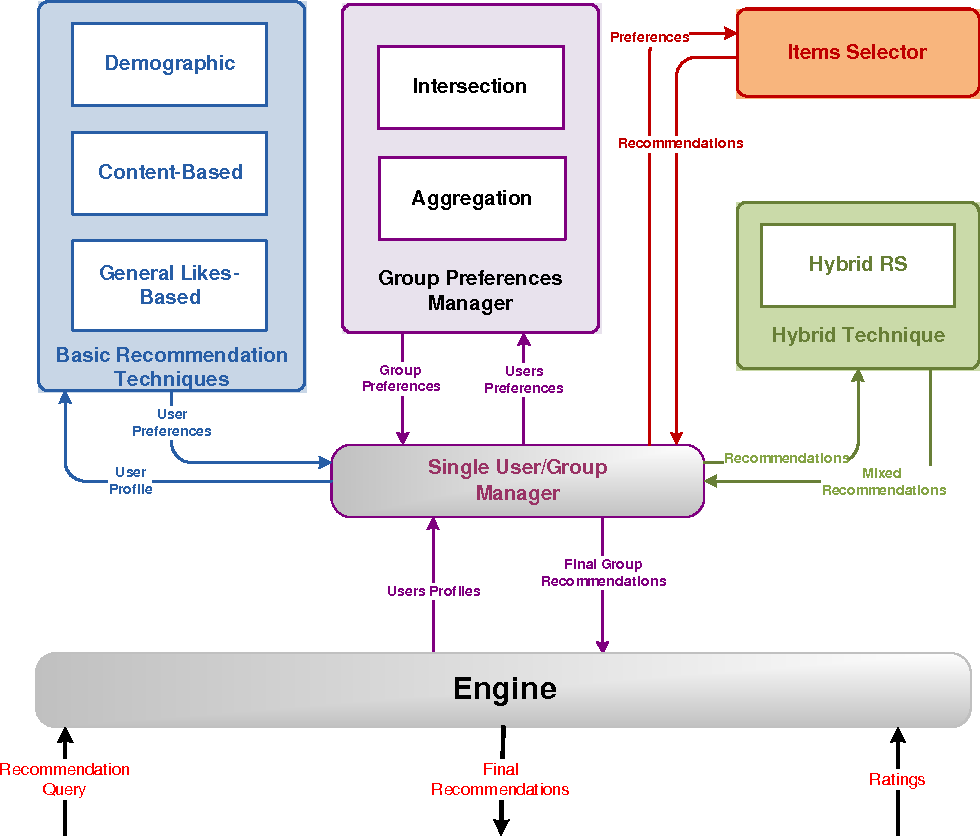
\includegraphics[width=400pt]{./images/2grsk.png}
\label{fig:2grsk}
\captionsource{GRSK Architecture from the Paper}{https://www.semanticscholar.org/paper/On-the-design-of-individual-and-group-recommender-Garcia-Sebastia/b367686e60db2f68102cd14b1360e9fc26a1757b}
\end{figure}\vspace{-24pt}
\vspace{1em}

This paper presents a recommender system for tourism based on the tastes of the users, their demographic classification, and the places they have visited on former trips. The system is able to offer recommendations for a single user or a group of users. The group recommendation is elicited out of the individual personal recommendations through the application of mechanisms such as aggregation and intersection. The elicitation mechanism is implemented as an extension of e-Tourism, a user-adapted tourism and leisure application whose main component is the Generalist Recommender System Kernel (GRSK), a domain-independent taxonomy-driven recommender system. \cite{ExpertSystemsWithApplications}

Compared to our system, the algorithm designed in this paper can be adapted with our group recommendation system. However, their study focuses on tourism but our system focuses on restaurant recommendation.

\newpage
\subsection{Dynamic Music Recommender System Using Genetic Algorithm}

%TODO heck for update
This paper represents a music recommendation system that is able to recognize and provide items corresponding with user favorites. The system is able to identify the n-number of users' preferences and adaptively recommend music tracks according to user preferences by extracting unique features of each music track. Then applying BLX-a crossover to the extracted features of each music track. \cite{MusicRecommender} The recommender is base on genetic algorithm along with content-based filtering technique for generate the initial population in genetic algorithm which can divided into 3 phase including feature extraction phase, evolution phase, and interactive Genetic algorithm phase. User favorite and user profiles are included. After that the successive page is constructed based on the user evaluation.

Compared to our system, the information of this paper that uses the genetic algorithm is similar to our system which are user favorite and user profiles. But the differences are our objective function and the system architecture in which we focus on the restaurant.


%%%%%%%%%%%%%%%%%%%%%%%%%%%%%%%%%%%%%%%%%%%%%%%%%%%%%%%%%%%%%%%%%%%%%%%%%%%%%%%%%%%%%%%%%%%%%%%%%%%%%%%%%%%%%%%%%%%%%%
%%%%%%%%%%%%%%%%%%%%%%%%%%%%%%%%%%%%%%%%%%%%%%%%%%%%%%%%%%%%%%%%%%%%%%%%%%%%%%%%%%%%%%%%%%%%%%%%%%%%%%%%%%%%%%%%%%%%%%
%%%%%%%%%%%%%%%%%%%%%%%%%%%%%%%%%%%%%%%%%%%%%%%%%%%%%%%%%%%%%%%%%%%%%%%%%%%%%%%%%%%%%%%%%%%%%%%%%%%%%%%%%%%%%%%%%%%%%%
%%%%%%%%%%%%%%%%%%%%%%%%%%%%%%%%%%%%%%%%%%%%%%%%%%%%%%%%%%%%%%%%%%%%%%%%%%%%%%%%%%%%%%%%%%%%%%%%%%%%%%%%%%%%%%%%%%%%%%
%%%%%%%%%%%%%%%%%%%%%%%%%%%%%%%%%%%%%%%%%%%%%%%%%%%%%%%%%%%%%%%%%%%%%%%%%%%%%%%%%%%%%%%%%%%%%%%%%%%%%%%%%%%%%%%%%%%%%%
%%%%%%%%%%%%%%%%%%%%%%%%%%%%%%%%%%%%%%%%%%%%%%%%%%%%%%%%%%%%%%%%%%%%%%%%%%%%%%%%%%%%%%%%%%%%%%%%%%%%%%%%%%%%%%%%%%%%%%


\chapter{Methodology and Design}

\section{System Functionality}
\subsection{Requirements}
\begin{itemize}
\item Users are able to register if they do not have an account.
\item Users are able to logout from our system.
\item An individual user is able to see the suggested restaurants.
\item Users are able to set restaurant preferences for each meal.
\item Users are able to see information about restaurants.
\item Users are able to select the restaurant that they want to go from the individual recommendation.
\item Users are able to rank the restaurants that they want to go by their preference from the group recommendation.
\item Users are able to join an eating group using a group pin code.
\item A group of users is able to start a group recommendation.
\item Users are able to save restaurants to their favorites and view them later.
\item Users are able to edit their food preferences.
\item The system must recommend restaurants to individuals and groups based on their preferences and behavior.
\item The system can suggest nearby restaurants based on users’ current location.
\end{itemize}


\newpage
\subsection{Use Case Diagram}

\begin{figure}[H]\centering
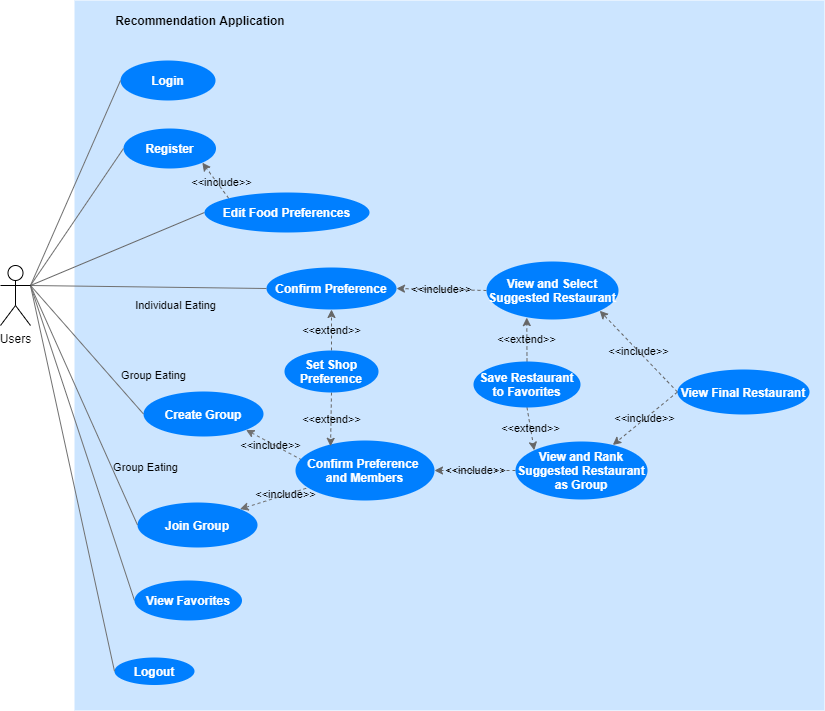
\includegraphics[width=440pt]{./images/3usecase.png}
\caption{Use Case Diagram}\label{fig:3usecase}
\end{figure}\vspace{-24pt}

\begin{enumerate}
\item Users can log in to the system using their username and password.
\item Users can register and users are required to set their food preference first before using the system.
\item Users can confirm the preference and see the suggested restaurants as individual eating and they can select the suggested restaurants. Moreover, users can save the restaurant into their favorite list.
\item Users can create a group or join other groups, then they can see the group confirmation page, and start the group recommendation.
\item Users can edit their food preference again.
\item Users can see their favorite list.
\item Users can log out from our system.
\end{enumerate}

\subsection{Use Case Narrative}
\subsubsection{Login}

\textbf{Name}: Users Login\\
\textbf{Actors}: Users\\
\textbf{Goal}: Users want to login into the system.\\
\textbf{Preconditions}: None\\
\textbf{Main Success Scenario}:\\
\textbf{1}. Users input their valid username and password.\\
\textbf{2}. User is logged in.\\
\textbf{Extensions (a)}\\
\textbf{1a}. Input username or password is not correct.\\
\textbf{2a}. System asks a user to input username and password again.\\
\textbf{3a}. Go back to the main scenario number 1.\\
\textbf{Extensions (b)}\\
\textbf{1b}. Input username or password is not correct.\\
\textbf{2b}. Users go to a registration page.\\
\textbf{Postconditions}: None

\subsubsection{Register}

\textbf{Name}: Users Login\\
\textbf{Actors}: Users\\
\textbf{Goal}: Users want to login into the system.\\
\textbf{Preconditions}: None\\
\textbf{Main Success Scenario}:\\
\textbf{1}. Users input their valid username and password.\\
\textbf{2}. User is logged in.\\
\textbf{Extensions (a)}\\
\textbf{1a}. Input username or password is not correct.\\
\textbf{2a}. System asks a user to input username and password again.\\
\textbf{3a}. Go back to the main scenario number 1.\\
\textbf{Extensions (b)}\\
\textbf{1b}. Input username or password is not correct.\\
\textbf{2b}. Users go to a registration page.\\
\textbf{Postconditions}: None

\subsubsection{Register}
\textbf{Name}: Users Registration\\
\textbf{Actors}: Users\\
\textbf{Goal}: Users do not have an account and want to use the system.\\
\textbf{Preconditions}: User open registration page.\\
\textbf{Main Success Scenario}: \\
\textbf{1}. System will show a general information form to the user.\\
\textbf{2}. Users fill the valid username and password in the general form.\\
\textbf{3}. Users fill all general fields in the general form.\\
\textbf{4}. Users confirm the general form.\\
\textbf{5}. System will ask the user to fill a food preference form.\\
\textbf{6}. Users fill the food preference form.\\
\textbf{7}. Users confirm the registration form.\\
\textbf{8}. User is registered and logged in.\\
\textbf{Extensions (a)} \\
\textbf{2a}. Username is invalid, already existed or password confirmation is mismatched.\\
\textbf{3a}. System asks the user to input a valid username and password again.\\
\textbf{4a}. Go back to the main scenario number 2.\\
\textbf{Extensions (b)} \\
\textbf{3b}. User didn’t fill some fields in the general form.\\
\textbf{4b}. Users confirm the general form.\\
\textbf{5b}. System asks the user to fill all the fields in the general form.\\
\textbf{6b}. Go back to the main scenario number 3.\\
\textbf{Postconditions}: None

\subsubsection{Individual Recommendation}
\textbf{Name}: Individual Recommendation\\
\textbf{Actors}: Users\\
\textbf{Goal}: Users want the system to suggest restaurants for them.\\
\textbf{Preconditions}: User is logged in and opens an individual recommendation page.\\
\textbf{Main Success Scenario}: \\
\textbf{1}. User allows the system to access their current location\\
\textbf{2}. The system shows a confirmation page to the user.\\
\textbf{3}. Users confirm the setting.\\
\textbf{4}. The system will show the suggested restaurant to the user\\
\textbf{5}. Users select the restaurant that they want to go to.\\
\textbf{6}. Users see their selected restaurant as a final restaurant.\\
\textbf{7}. Recommendation completed\\
\textbf{Extensions (a)} \\
\textbf{1a}. Users do not allow the system to access their current location.\\
\textbf{2a}. The nearby restaurant suggestion will be disabled.\\
\textbf{3a}. Continue to the main scenario number 2.\\
\textbf{Extensions (b)} \\
\textbf{2b}. Users change the setting for that meal.\\
\textbf{3b}. Go back to the main scenario number 3.\\
\textbf{Extensions (c)} \\
\textbf{4c}. Users save the restaurant to their favorite list.\\
\textbf{5c}. Go back to the main scenario number 5.\\
\textbf{Postconditions}: None

\subsubsection{Group Recommendation}
\textbf{Name}: Group Recommendation\\
\textbf{Actors}: Users\\
\textbf{Goal}: Users want the system to suggest restaurants for their group.\\
\textbf{Preconditions}: Users are logged in and open a group recommendation page.\\
\textbf{Main Success Scenario}: \\
\textbf{1}. Users allow the system to access their current location.\\
\textbf{2}. Users see the confirmation page and group pin code.\\
\textbf{3}. Users share pin code or QR code to others members.\\
\textbf{4}. Every member joined.\\
\textbf{5}. Head of the party selects to start the recommendation.\\
\textbf{6}. Everybody in the group sees the same set of the restaurants.\\
\textbf{7}. Everybody selects their restaurant they want to go to by their preference.\\
\textbf{8}. Everybody finished selecting the restaurants.\\
\textbf{9}. The system shows the final restaurant to the group.\\
\textbf{9}. Recommendation completed\\
\textbf{Extensions (a)} \\
\textbf{3a}. Users choose to join the group by inputting the group pin.\\
\textbf{4a}. Group pin is invalid.\\
\textbf{5a}. Users cannot join the invalid pin group.\\
\textbf{Extension (b)} \\
\textbf{6b}. Users save the restaurant to their favorite list.\\
\textbf{7b}. Continue to the main scenario number 7\\
\textbf{Postconditions}: None

\subsubsection{Edit the Food Preference}
\textbf{Actors}: Users\\
\textbf{Goal}: Users want to edit their food preference.\\
\textbf{Preconditions}: Users are logged in.\\
\textbf{Main Success Scenario}: \\
\textbf{1}. Users choose to edit their food preference.\\
\textbf{2}. The old food preference will be shown and let users edit them.\\
\textbf{5}. User confirm the modification\\
\textbf{Postconditions}: None

\subsubsection{See the Favorite List}
\textbf{Actors}: Users\\
\textbf{Goal}: Users want to see their restaurant favorite list.\\
\textbf{Preconditions}: Users are logged in\\
\textbf{Main Success Scenario}: \\
\textbf{1}. Users choose to see their favorite list.\\
\textbf{2}. The system shows a list of their favorite restaurants to the users.\\
\textbf{3}. Users see their favorite list.\\
\textbf{Extensions (a)} \\
\textbf{3a}. Users choose to remove the restaurant from their favorite list.\\
\textbf{4a}. The restaurant is removed from their favorites list.\\
\textbf{Postconditions}: None

\subsubsection{Logout}
\textbf{Name}: Users Logout\\
\textbf{Actors}: Users\\
\textbf{Goal}: Users want to logout from the system.\\
\textbf{Preconditions}: Users are logged in.\\
\textbf{Main Success Scenario}: \\
\textbf{1}. User choose to logout\\
\textbf{2}. User is logged out\\
\textbf{Postconditions}: None


\newpage
\subsection{Functional Breakdown Structure}
\begin{figure}[H]\centering
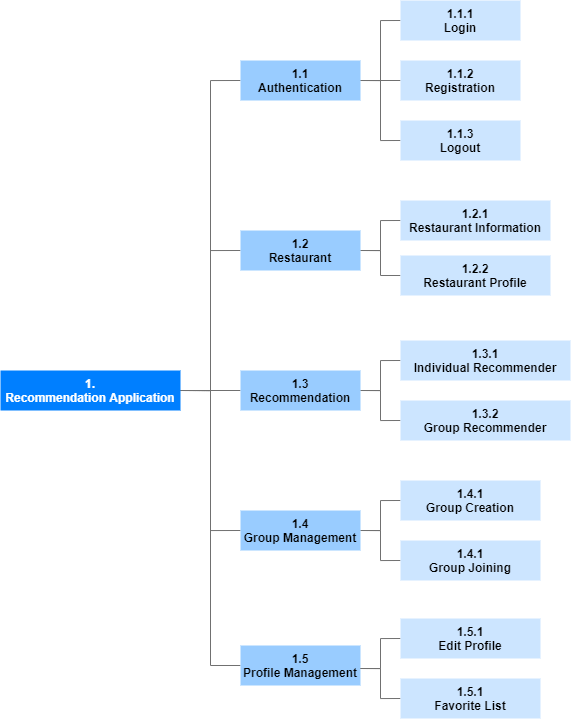
\includegraphics[width=360pt]{./images/3functional_breakdown.png}
\caption{Functional Breakdown Structure of the System}\label{fig:3functional_breakdown}
\end{figure}\vspace{-24pt}

Our system consists of 5 functional components which are:

\begin{enumerate}
\item Authentication, it handles user registration, login, and logout.
\item Restaurant, it serves the restaurant information and their profile which include restaurant categories, price and distance.
\item Recommendation, it generates the restaurant recommendation which is separated into individual and group recommendation.
\item Group Management, manages the group used in group recommendation.
\item Profile Management, manages the user profile and their favorite list.
\end{enumerate}


\section{System Architecture}
\subsection{System Overview}
\begin{figure}[H]\centering
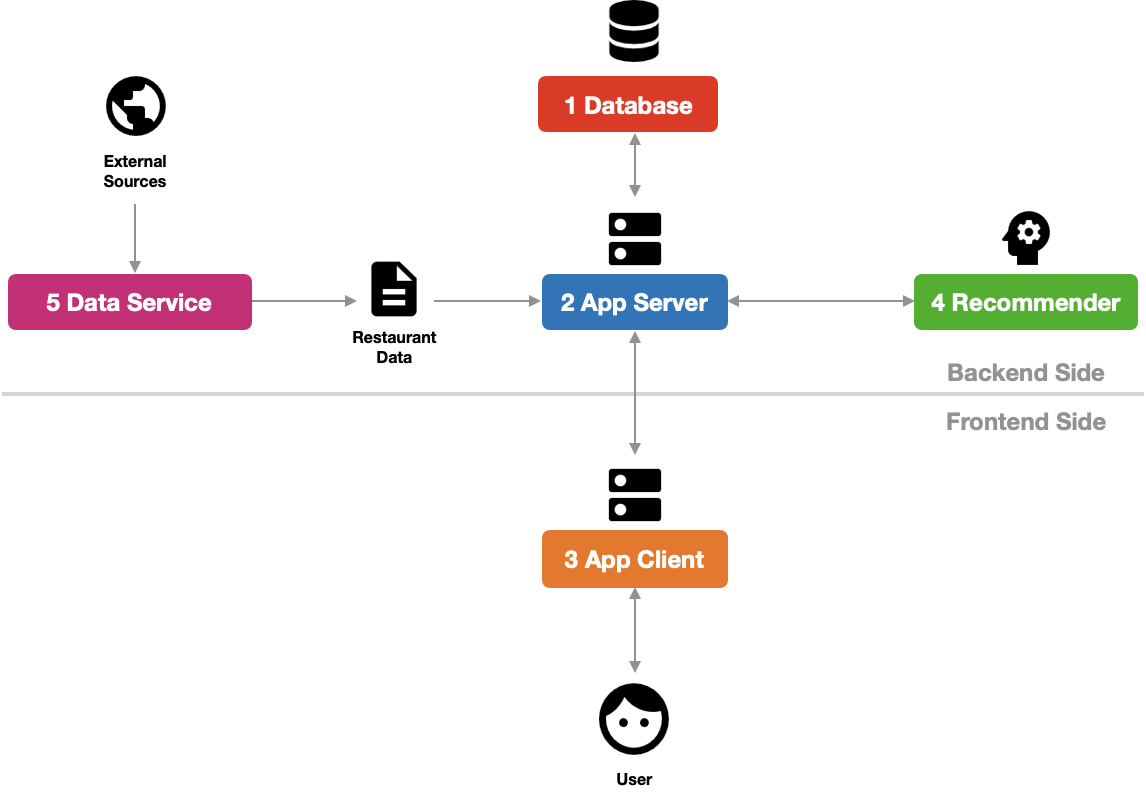
\includegraphics[width=360pt]{./images/3system_overview.png}
\caption{System Overview}\label{fig:3system_overview}
\end{figure}\vspace{-24pt}

In this section, we will give an overview of our system about their responsibility and we will discuss each component in detail in the next section.

From Figure~\ref{fig:3system_overview}, we can see the relationship between each component. Our system consists of mainly 5 components which are \textit{Database}, \textit{App Server}, \textit{App Client}, \textit{Recommender}, and \textit{Data Service}.

%TODO Italic specific name
\begin{itemize}
\item \textit{Database}: store all of the data of our system.
\item \textit{App Server}: handle all server-side processes including restaurant data management, group management, recommendation request handling, and authentication system. This component acts as a center of the system.
\item \textit{App Client}: serve the user interface to users via a web application.
\item \textit{Recommender}: handle the restaurant's suggestion. This component will receive the recommendation request from \textit{App Server} and return the suggestion result back to \textit{App Server}.
\item \textit{Data Service}: collect restaurant data from external sources, preprocess the data, and feed the data into \textit{App Server}.
\end{itemize}

We separate these components into 2 sides which are the backend side and the frontend side. The backend side includes \textit{Database}, \textit{App Server}, \textit{Recommender}, and \textit{Data Service}. The frontend side is only \textit{App Client}.


\newpage
\subsection{Restaurant Recommender System Architect}

\begin{figure}[H]\centering
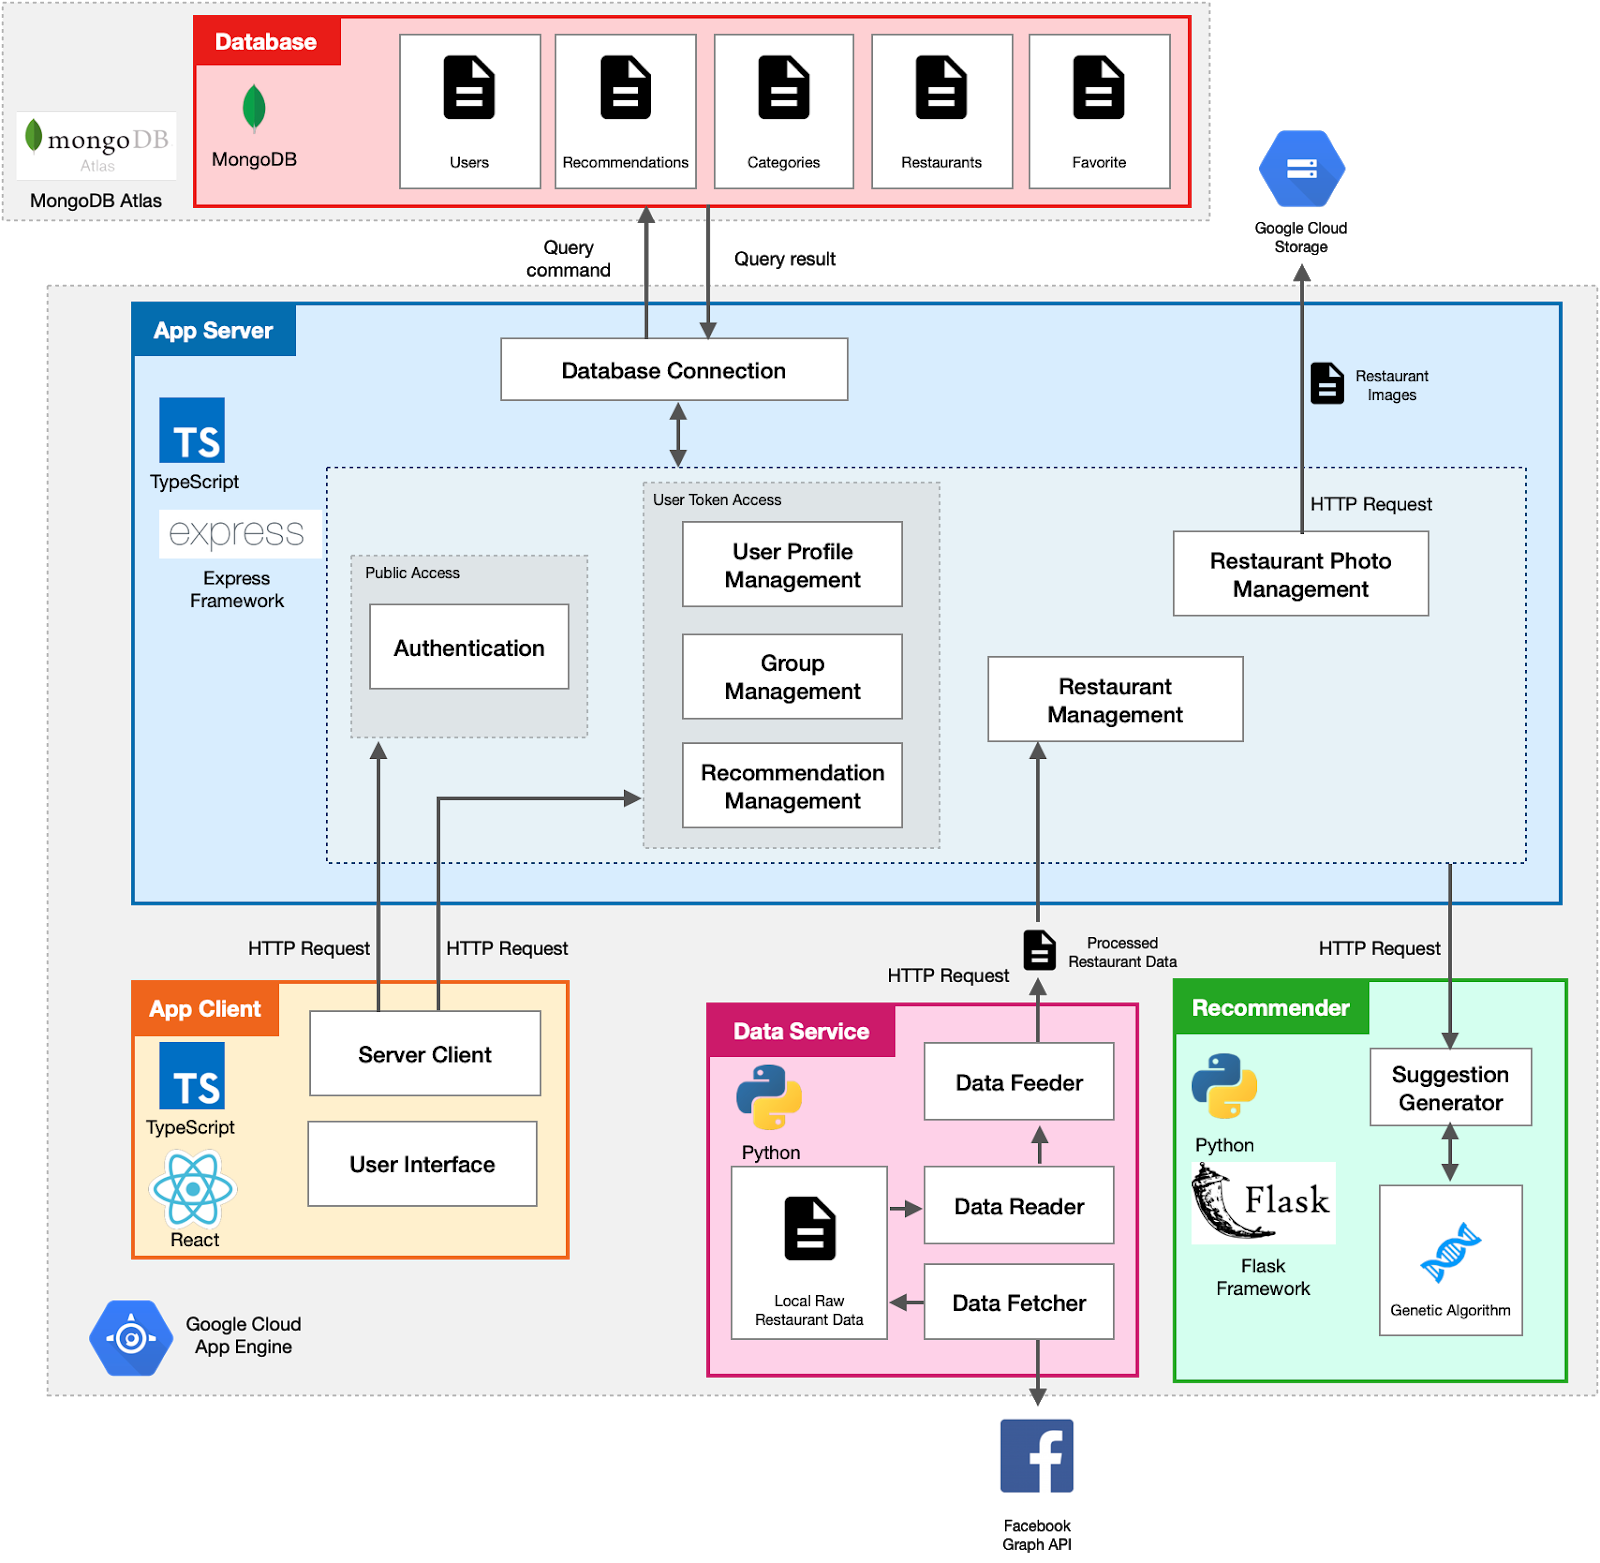
\includegraphics[width=400pt]{./images/3architect.png}
\caption{System Architecture}\label{fig:3architect}
\end{figure}\vspace{-24pt}

Figure~\ref{fig:3architect} shows the detailed architecture of our system. As we mentioned before, our system consists of 5 components. Each of these components communicates via HTTP request and response. All of the components except \textit{Database} are deployed using Google Cloud App Engine and \textit{Database} is deployed via MongoDB Atlas. There are 3 external services that our system needs to be interacted with which are Google Cloud Storage, Facebook Graph API and Longdo Map API. Google Cloud Storage is used for storing restaurant’s images. Facebook Graph API is used for querying primary restaurant information. Longdo Map API is used to query places by keywords. We will walk through each component in detail in the following section.

\newpage
\subsubsection{App Server Architecture}

\begin{figure}[H]\centering
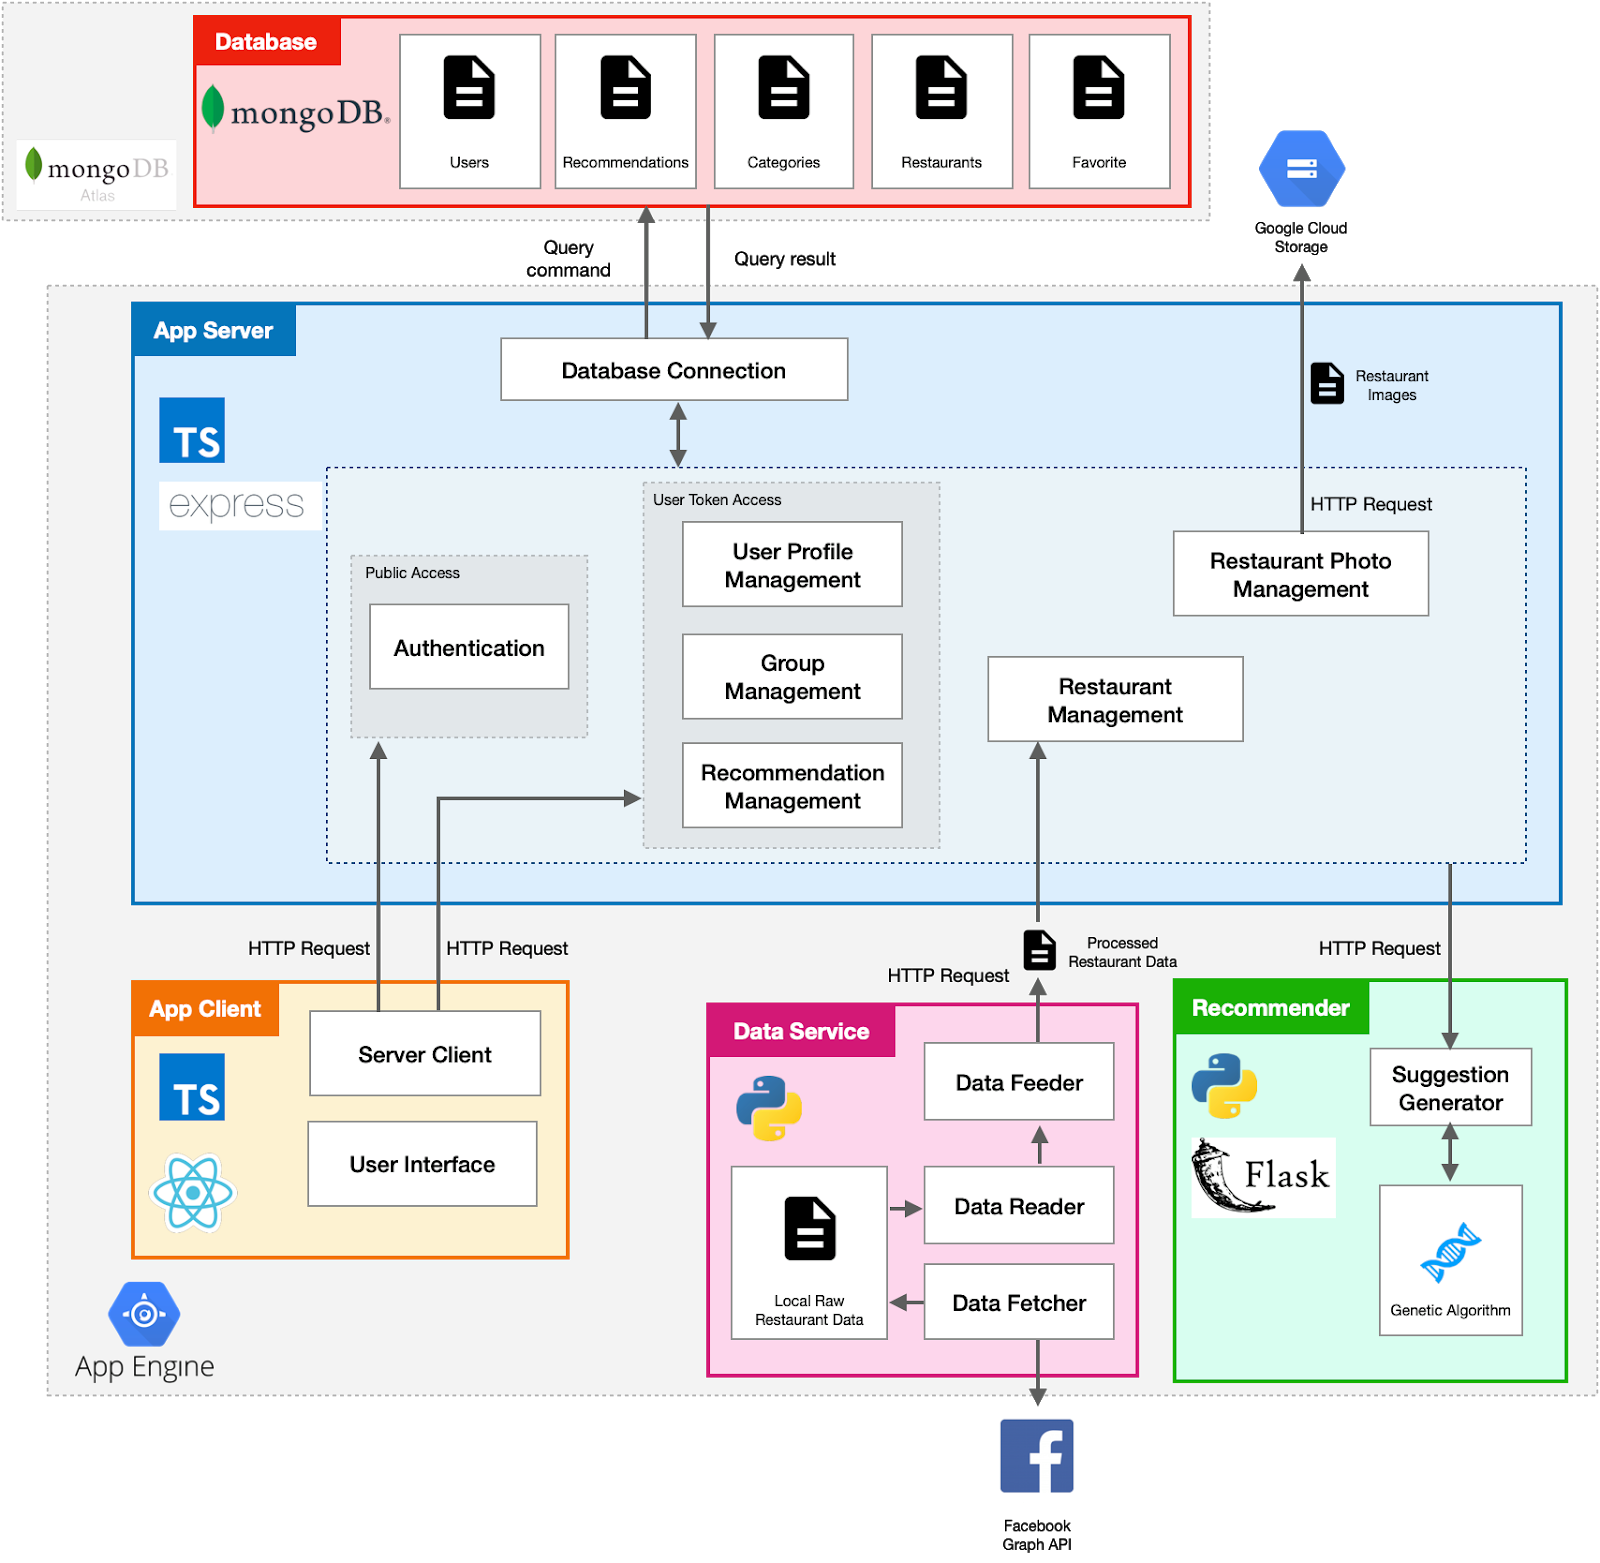
\includegraphics[width=360pt]{./images/3arch_appserver.png}
\caption{App Server Architecture}\label{fig:3arch_appserver}
\end{figure}\vspace{-24pt}

\textit{App Server} is responsible for handling all server-side processes. The processes include authentication, user management, group management, recommendation management, restaurant management, and model management. This component acts as a center of our system that lets all other components communicate with them.

For database communication, this is the only component that allows access to the database, so any components needed to access any data must communicate through \textit{App Server}. The database connection module acts as an interface to the database for \textit{App Server}.

For an \textit{App Client} communication, \textit{App Client} needs to send a request to \textit{App Server} in order to complete a task. The requests include authentication requests, create and update a recommendation request, get, create, and update group requests and get, create, and update user information requests.

For a \textit{Data Service} communication, \textit{Data Service} generates processed restaurant data and it sends those data to \textit{App Server} to create a restaurant and store them in the database.

For a \textit{Recommender} communication, \textit{App Server} needs to send requests to \textit{Recommender} for restaurant suggestion generation and model training. \textit{Recommender} also needs to send a request to \textit{App Server} to get restaurant information and user information.

There are also two external services that \textit{App Server} needs to communicate with which are Google Cloud Storage and Longdo Map API. With Google Cloud Storage service, \textit{App Server} will send a request to store the restaurant’s images and get the existing image from that service. With Longdo Map API, \textit{App Server} will send places query requests with specific keywords from users. 

\textit{App Server} is implemented using TypeScript and Express framework which is a web application framework and deployed on Google Cloud App Engine service.


\subsubsection{App Client Architecture}

\begin{figure}[H]\centering
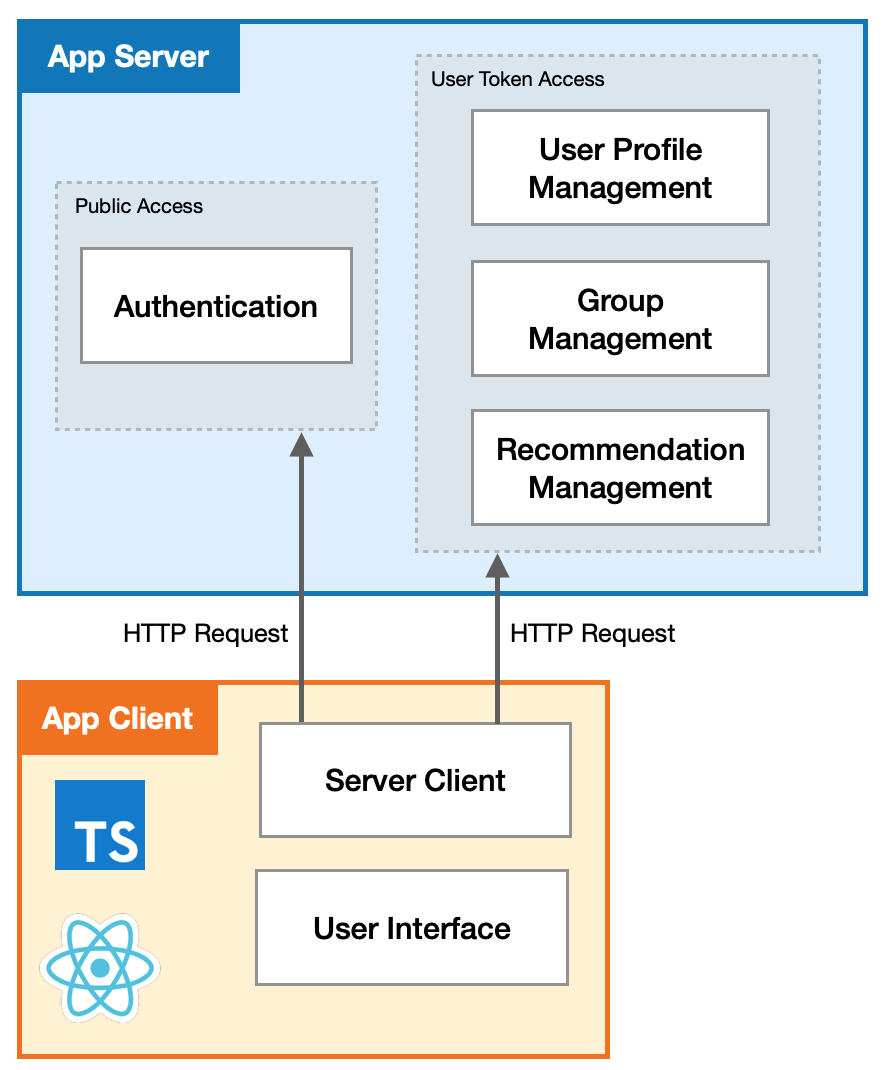
\includegraphics[width=200pt]{./images/3arch_appclient.png}
\caption{App Client Architecture}\label{fig:3arch_appclient}
\end{figure}\vspace{-24pt}

\textit{App Client} is responsible for serving the user interface to users and handling user interactions. There are 2 modules in this component which are User Interface that serves as an interface to users and Server Client that handles user’s tasks and communicates with \textit{App Server}. \textit{App Client} is implemented using TypeScript and React framework and deployed on Google Cloud App Engine service.


\subsubsection{Recommender Architecture}

\begin{figure}[H]\centering
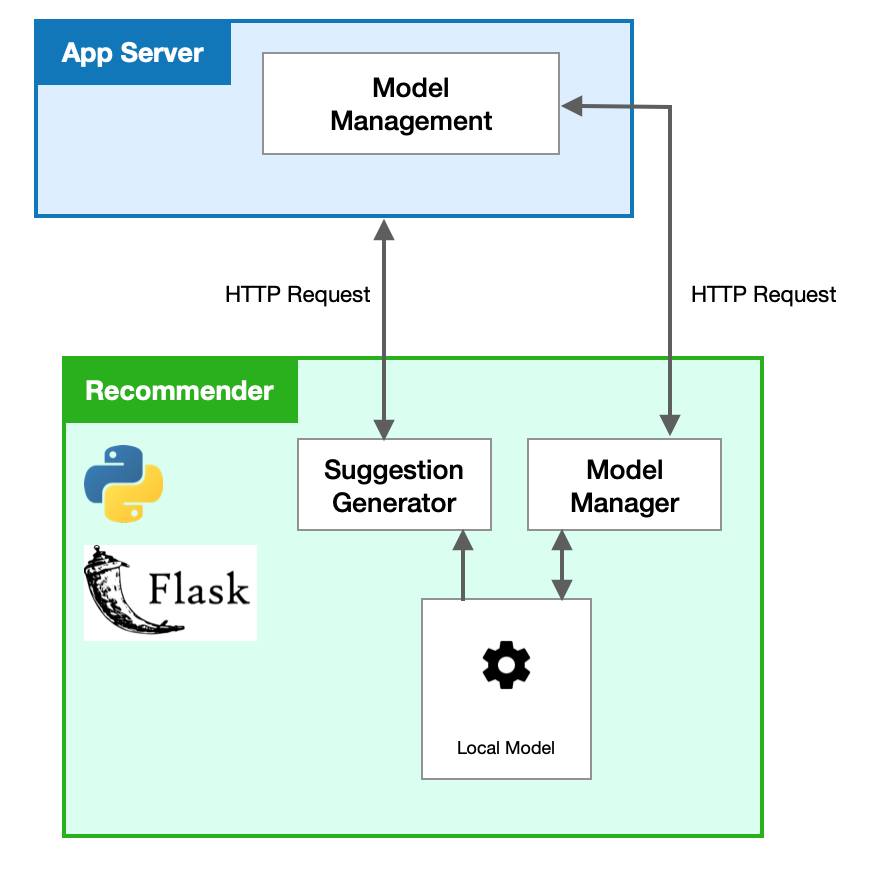
\includegraphics[width=200pt]{./images/3arch_recommender.png}
\caption{Recommender Architecture}\label{fig:3arch_recommender}
\end{figure}\vspace{-24pt}

\textit{Recommender} is responsible for restaurant suggestion generation. There are 2 modules in this component which are Suggestion Generator and Model Manger.

Suggestion Generator will receive a recommendation request from \textit{App Server}, generate one set of restaurants using a local model, and send that response back to \textit{App Server}. In this process, \textit{Recommender} also needs to get some information about restaurants and users from \textit{App Server} for the generation.

Model Manager will manage the local model. It is waiting for a training request from \textit{App Server} to train a new local model. It also sends the training information request back to \textit{App Server} after the training process is finished.

\textit{Recommender} implemented using Python which can easily communicate with the model because many libraries are supporting the machine learning process. It also uses the Flask framework to make them listen for requests from \textit{App Server}. It is deployed on the Google Cloud App Engine service.


\subsubsection{Data Service Architecture}

\begin{figure}[H]\centering
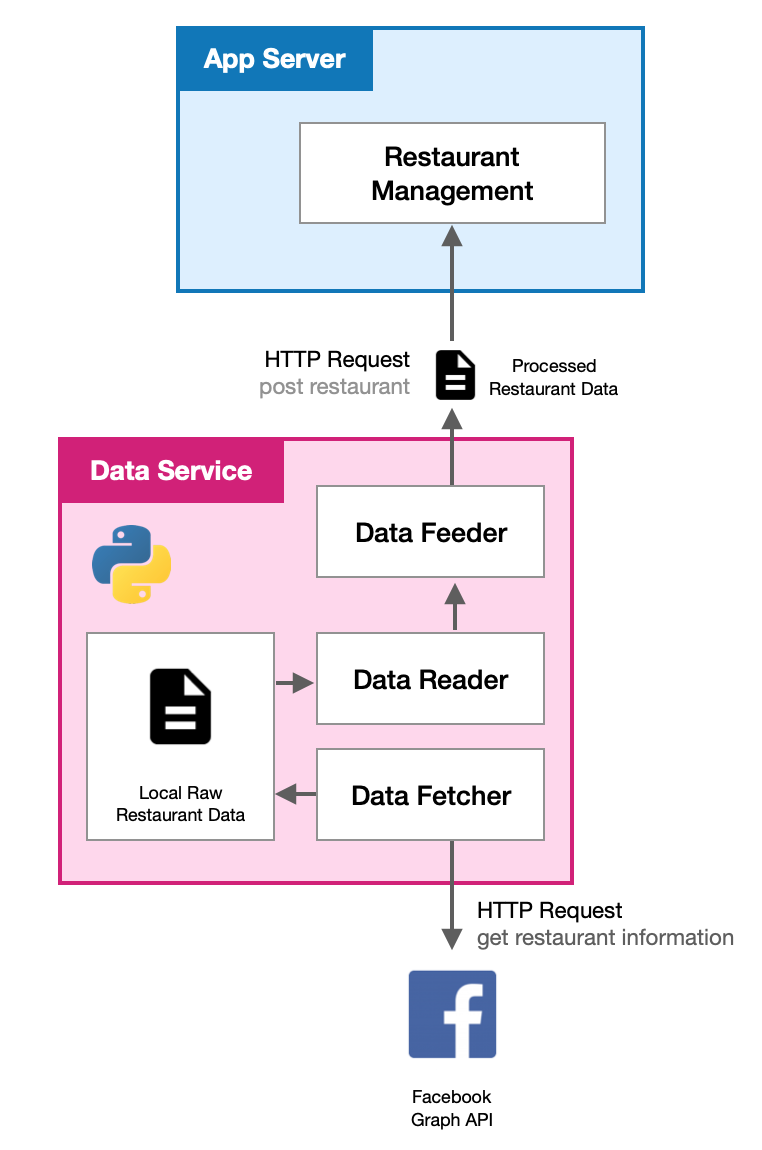
\includegraphics[width=200pt]{./images/3arch_dataservice.png}
\caption{Data Service Architecture}\label{fig:3arch_dataservice}
\end{figure}\vspace{-24pt}

\textit{Data Service} is responsible for collecting restaurant information from an external source. This component has 3 modules which are Data Fetcher which collect the restaurant information from Facebook Graph API and save it to the local raw files, Data Reader which will read the files and process that data into the correct format and Data Feeder will send the processed data to \textit{App Server} to create restaurants in the system. Currently, it is designed to collect the restaurant data manually. Therefore, if we want to update or collect more restaurants, we need to trigger the task in this service again. \textit{Data Service} is implemented as a simple Python script without any web framework because no components need to send a request to \textit{Data Service}.

\subsubsection{Database Architecture}

\begin{figure}[H]\centering
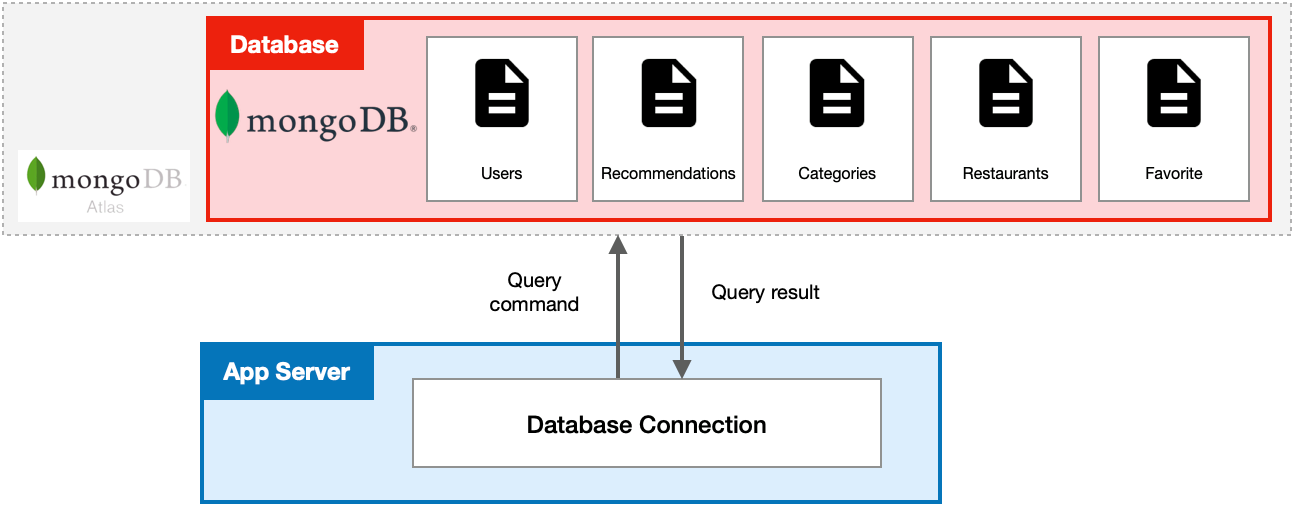
\includegraphics[width=400pt]{./images/3arch_database.png}
\caption{App Server Architecture}\label{fig:3arch_database}
\end{figure}\vspace{-24pt}

\textit{Database} is responsible for storing all data in our system. We choose to have NoSQL for our database because the schema of the data can change quickly, having a flexible schema can make our system adapt to the change in data format more easily. We will discuss the database structure in section~\ref{sec:databasestructure} Database Structure. To access the data in the database, \textit{App Server} will send a query command via the database connection module in \textit{App Server}. The database is implemented using MongoDB and deployed using their official cloud service, MongoDB Atlas.


\newpage
\section{User Journey}

\subsection{Activity Diagrams}

\subsubsection{Registration}

\begin{figure}[H]\centering
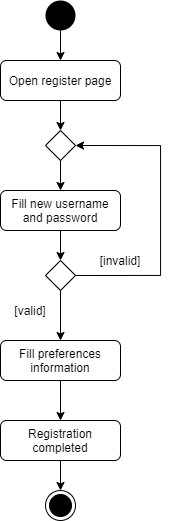
\includegraphics[height=400pt]{./images/3actdiagram_register.png}
\caption{Registration Activity Diagram}\label{fig:3actdiagram_register}
\end{figure}\vspace{-24pt}

When users open a registration page, they will be asked to input their new username and password. If their new username and password are valid they need to fill in the food preferences information. Then the registration will be completed.

\newpage
\subsubsection{Individual Restaurant Recommendation}

\begin{figure}[H]\centering
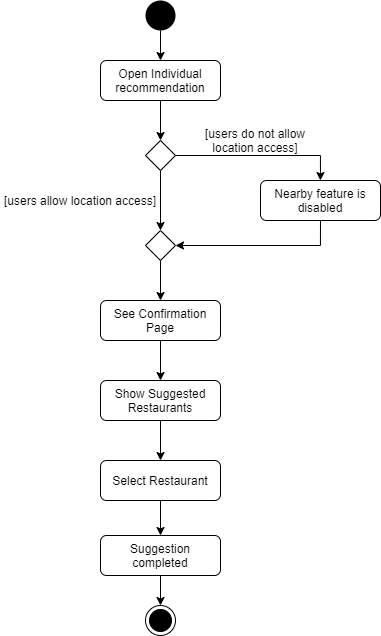
\includegraphics[height=400pt]{./images/3actdiagram_indirec.png}
\caption{Individual Restaurant Recommendation Activity Diagram}\label{fig:3actdiagram_indirec}
\end{figure}\vspace{-24pt}

When users choose to start the individual recommendation, users need to allow their current location access in order to use nearby suggestion features. And before entering the recommendation, they will see the confirmation page which they can configure the setting and location. After that, they will see the suggested restaurant and can optionally save any restaurant into their favorite list. If they are satisfied with the suggestion and select the final restaurant, the recommendation will be completed. Otherwise, users can choose to see more suggestions.

\newpage
\subsubsection{Registration}

\begin{figure}[H]\centering
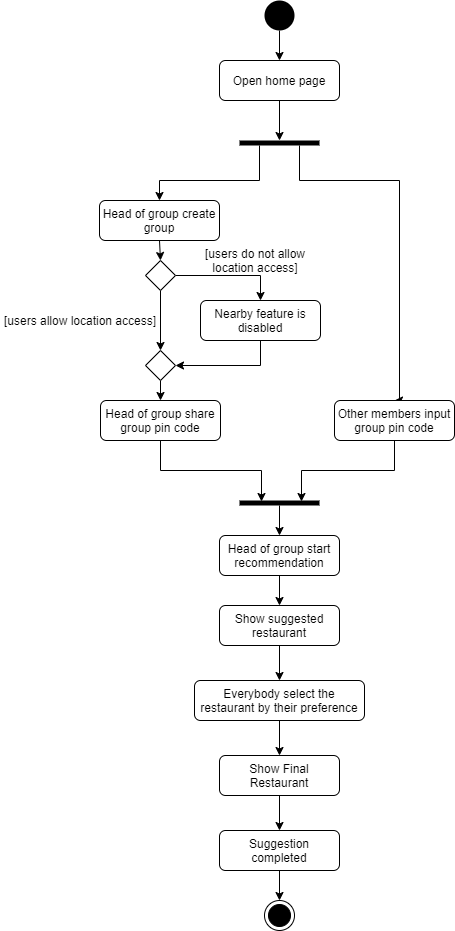
\includegraphics[height=400pt]{./images/3actdiagram_grouprec.png}
\caption{Group Restaurant Recommendation Activity Diagram}\label{fig:3actdiagram_grouprec}
\end{figure}\vspace{-24pt}

When a group of users wants to start a group recommendation, they firstly need to create a group and let other members join the group. This requires only one member to create a group and that person will be a head of the party which they can change the location and main configuration. Other members can use the group pin code shared by the head or other members that are already in the group. After the head chooses to start the recommendation, the same set of restaurants will be shown to all members. Everybody then needs to rank the restaurants that they want to go to by their preference. After everybody is done selecting their restaurants, the final suggested restaurant will be shown to the group and the recommendation is completed.


\newpage
\subsection{Sequence Diagrams}

\subsubsection{Registration}

\begin{figure}[H]\centering
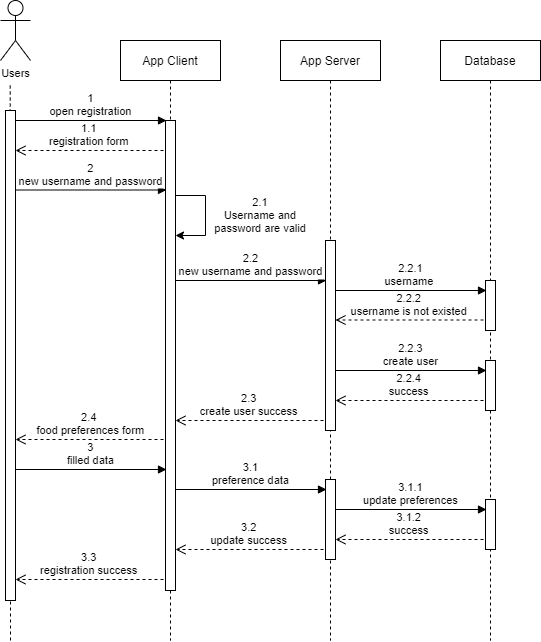
\includegraphics[height=400pt]{./images/3seqdiagram_register.png}
\caption{Registration Sequence Diagram}\label{fig:3seqdiagram_register}
\end{figure}\vspace{-24pt}

\textbf{Scenario}: Users register for a new account.
\begin{enumerate}
\item Users open the registration page and \textit{App Client} shows the registration form to users.
\item Once users fill in their new username and password, \textit{App Client} will validate the username format (2.1). If they are valid, \textit{App Client} will send those fields to the app server (2.2). Next, \textit{App Server} will query the username from the database (2.2.1). If the username does not exist in the database, the new user will be created (2.2.4) and sent back to \textit{App Client} (2.3). The \textit{App Client} will send a food preference setting form to the users (2.4).
\item Once users fill the food preferences setting form, the user profile in the database will be updated (3.1.2) and the registration will be completed (3.3)
\end{enumerate}


\newpage
\subsubsection{Individual Restaurant Recommendation}

\begin{figure}[H]\centering
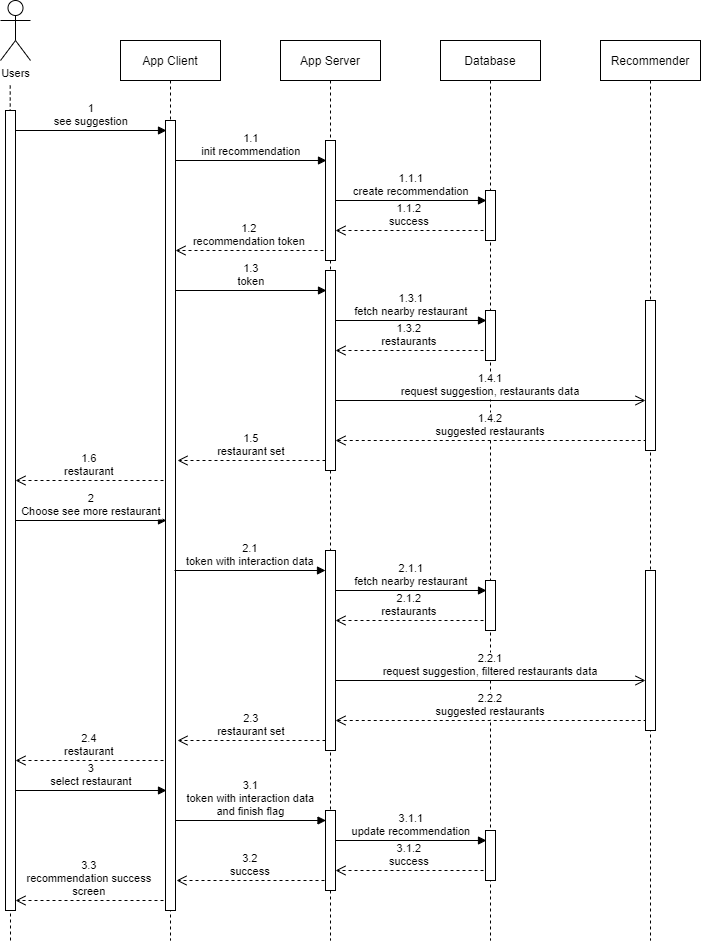
\includegraphics[height=600pt]{./images/3seqdiagram_indirec.png}
\caption{Individual Restaurant Recommendation Sequence Diagram}\label{fig:3seqdiagram_register}
\end{figure}\vspace{-24pt}

\newpage
\textbf{Scenario}: Users want to see the restaurant recommendation for individuals and they want to see more suggestions than the first set of the suggested restaurants.
\begin{enumerate}
\item When users want to see a recommendation, \textit{App Client} will send an initial recommendation request to the \textit{App Server} (1.1), \textit{App Server} will create a new recommendation data (1.1.1 and 1.1.2) and send the recommendation back to \textit{App Client} (1.2). Next, \textit{App Client} will send the token to \textit{App Server} again (1.3). Once \textit{App Server} receives the token, it will fetch nearby restaurants (1.3.1 and 1.3.2) and send a recommendation request with the restaurants to \textit{Recommender} (1.4.1). \textit{Recommender} will generate a set of suggested restaurants and send them back to \textit{App Server} and \textit{App Client} (1.4.2 and 1.5). Lastly, \textit{App Client} will show a restaurant in the restaurant set to users  (1.6).
\item Users will see the suggested restaurants. In this scenario, users choose to see more suggested restaurants (2). After that \textit{App Client} will send a recommendation token with current restaurants interaction data to filter out the suggested restaurants in the first set (2.1). The next process is generating a restaurant suggestion which is the same process as before, but this time, \textit{App Server} will send only the filtered restaurants to \textit{Recommender} (2.2.1). After the suggestion is generated, it will be sent back to \textit{App Server}, \textit{App Client} and users (2.2.2, 2.3, and 2.4).
\item When users select the restaurant from the set (3) which means the recommendation is finished, \textit{App Client} will send the recommendation token with a finish flag to \textit{App Server} (3.1). \textit{App Server} will send an update request to \textit{Database} (3.1.1) and after its success, the recommendation success screen will be shown to users (3.3).
\end{enumerate}



\newpage

\subsubsection{Create Group}

\begin{figure}[H]\centering
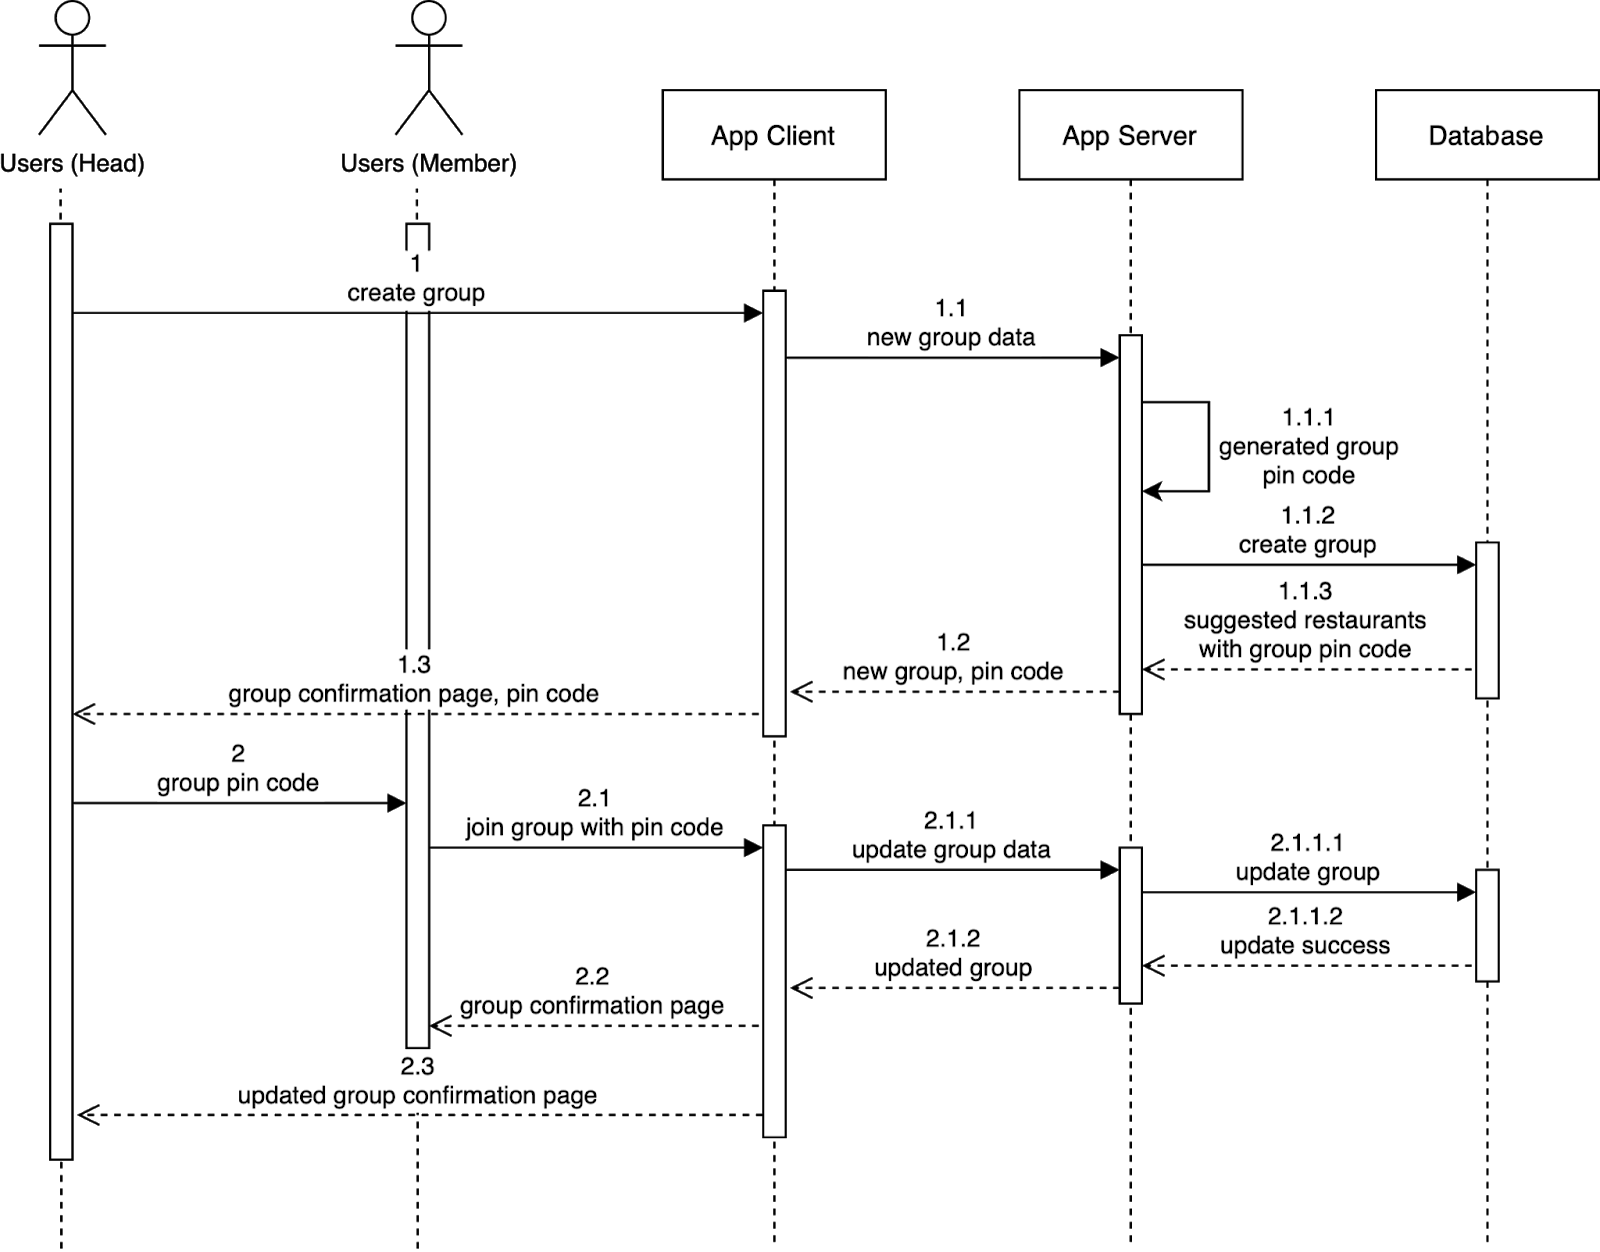
\includegraphics[width=400pt]{./images/3seqdiagram_creategroup.png}
\caption{Create Group Sequence Diagram}\label{fig:3seqdiagram_creategroup}
\end{figure}\vspace{-24pt}

\textbf{Scenario}: A group of 2 people wants to create a new eating group by the first user creating a group and the other one joining the group.
\begin{enumerate}
\item The first member creates a group (1). \textit{App Client} sends data to \textit{App Server} (1.1). \textit{App Server} generates a group pin code (1.1.1) and creates a new record in the database (1.1.2). Finally, the member will see a group confirmation page and a group pin code (1.3).
\item After the member has the group pin code, they can share it to other members (2). When other members join a group with a pin code (2.1), \textit{App Server} will update the record in the database (2.1.1) and other members will see the same group confirmation page as the person who created a group (2.2). The group information of the first member will also be updated (2.3).
\end{enumerate}


\newpage

\subsubsection{Group Restaurant Recommendation}

\begin{figure}[H]\centering
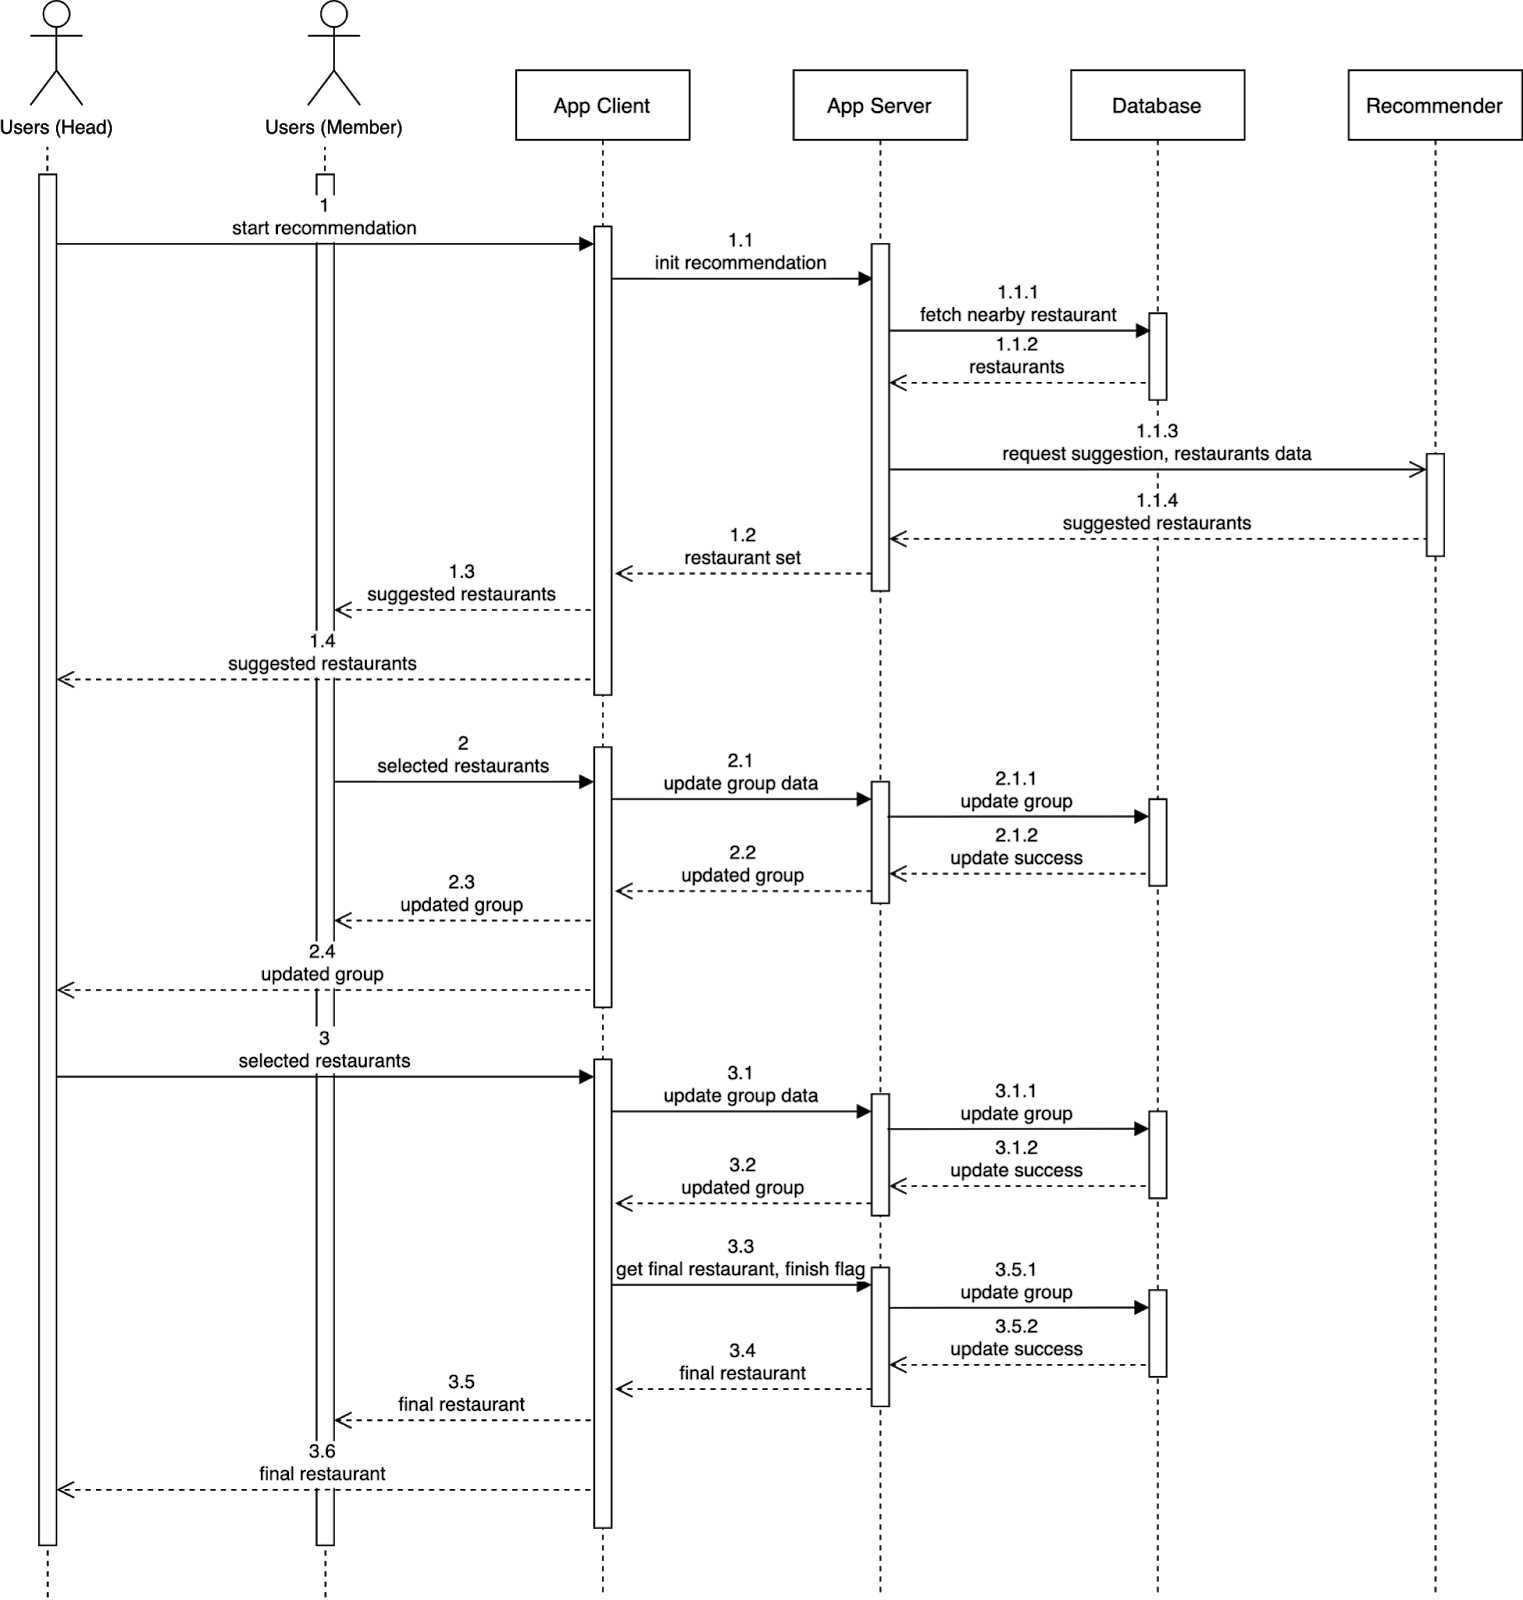
\includegraphics[width=400pt]{./images/3seqdiagram_grouprec.png}
\caption{Create Group Sequence Diagram}\label{fig:3seqdiagram_grouprec}
\end{figure}\vspace{-24pt}

\newpage
\textbf{Scenario}: A group of 2 people wants to have a restaurant recommendation for their group and they already have a group created.
\begin{enumerate}
\item When a head of the group which is the first member who created the group chooses to start a recommendation (1), \textit{App Client} will request a new group recommendation to \textit{App Server} (1.1). After that \textit{App Server} and \textit{Recommender} will generate a suggestion which has the same process as the individual recommendation (1.1.1 to 1.1.4). Note that \textit{Recommender} can handle multiple users in the recommendation. Finally, the same suggested restaurant set will be shown to all members (1.3 and 1.4).
\item The first member finishes selecting their restaurant by their preference (2). \textit{App Server} will update a group data (2.1) and both of the members will receive the update group data (2.3 and 2.4). However, the recommendation is not completed yet, it needs to wait for the other member to finish selecting the restaurants.
\item The second member finishes selecting the restaurants (3). \textit{App Server} will update a group data again (3.1). In this time, \textit{App Client} detects that every member has finished selecting the restaurant, so it will send a group finalization request with a finish flag (3.3). \textit{App Server} will finalize the final restaurant to the group (3.3.1) and update the group data again (3.3.2). Finally, the final restaurant will be shown to every member (3.5 and 3.6) and the recommendation will be completed.
\end{enumerate}


\section{User Interface Design}
This section presents the user interface design of the restaurant recommendation system which designs in the Figma application.

The user interface of our web application includes login, registration, individual restaurant recommendation, group restaurant recommendation, and users’ profile as follows.

\newpage
\subsubsection{Login Page}
\begin{figure}[H]\centering
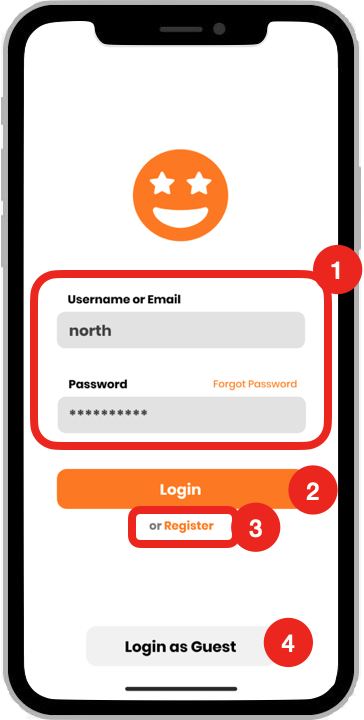
\includegraphics[height=300pt]{./images/3ui_StartPageUserInterfaceDesign.png}
\caption{Start Page User Interface Design}\label{fig:3ui_StartPageUserInterfaceDesign}
\end{figure}\vspace{-24pt}

\begin{enumerate}
\item Username and password input fields
\item Login button to confirm the input fields
\item Register button, it links to the registration page
\item Login as Guest for users who do not want an account but want to start using our system right away.
\end{enumerate}

When users open the application, the login page will appear first if they did not login yet. They need to input their username and password in the fields (1) then They can tap the “Login” button (2) to log in. After login, they will see the home page (Figure~\ref{fig:3ui_HomePageUserInterfaceDesign}). If they do not have an account, they can tap on the “Register” button (3) and they will see the registration page (Figure~\ref{fig:3ui_RegistrationPageUserInterfaceDesign}). However, they can choose to login without any account by tapping on the “Login as Guest” button (4) and the system will directly bring them to the home page (Figure~\ref{fig:3ui_HomePageUserInterfaceDesign}).

\newpage
\subsubsection{Registration Page}
\begin{figure}[H]\centering
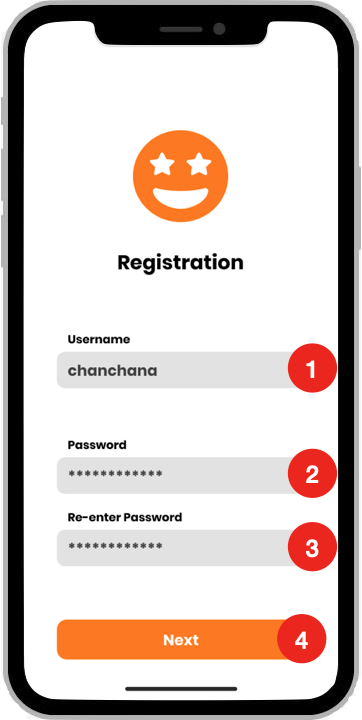
\includegraphics[height=300pt]{./images/3ui_RegistrationPageUserInterfaceDesign.png}
\caption{Registration Page User Interface Design}\label{fig:3ui_RegistrationPageUserInterfaceDesign}
\end{figure}\vspace{-24pt}

\begin{enumerate}
\item New username field
\item New password field
\item Re-enter the password field, it needs to be matched with the password field
\item Next button, links to a general information setup page
\end{enumerate}

If users choose to register, the registration page will appear and ask users to input a new username, password, and re-enter the password (1), (2), (3) respectively. If the input username is invalid or already taken, the system will alert users and let them choose a new username. If the password field and re-enter password field are mismatched, the system will also alert and tell users to input their password and re-enter password fields again. After all of the information in the fields is valid and users tap on the “Next” button (4), they will proceed to the next step which is the profile setting step stated in Figure~\ref{fig:3ui_ProfileSetupPageUserInterfaceDesign}.

\newpage
\begin{figure}[H]\centering
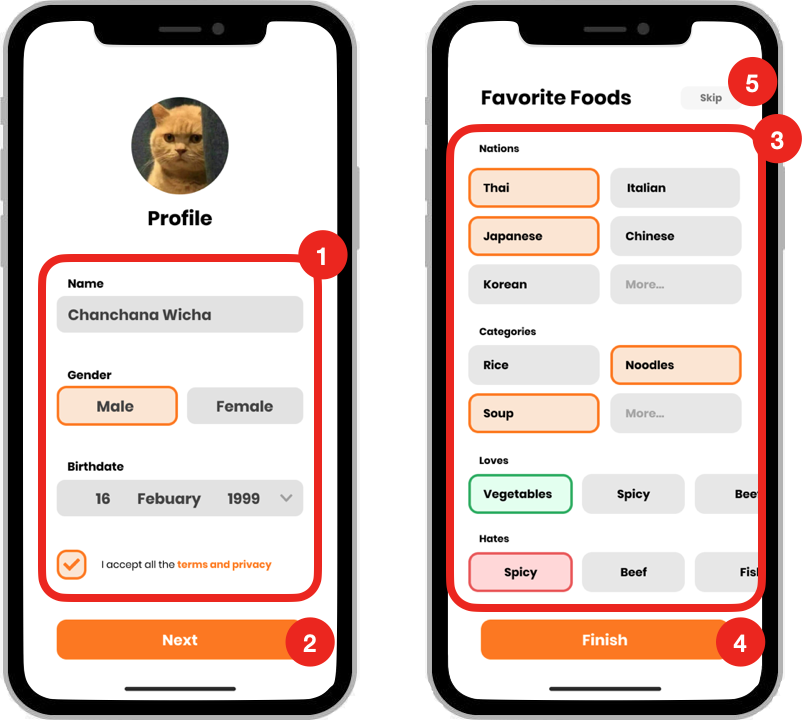
\includegraphics[height=300pt]{./images/3ui_ProfileSetupPageUserInterfaceDesign.png}
\caption{Profile Setup Page User Interface Design}\label{fig:3ui_ProfileSetupPageUserInterfaceDesign}
\end{figure}\vspace{-24pt}

\begin{enumerate}
\item General information form
\item Next button, will proceed users to the food preference setup step
\item Food preference form, let users choose their food preference in each category.
\item Finish button, to complete the form and the registration.
\item Skip button, lets users skip the food preference setup process.
\end{enumerate}

After users input the valid username and password, the next step is user profile setup. This process consists of 2 steps which are general information setup and food preferences information setup. The first one on the left of Figure~\ref{fig:3ui_ProfileSetupPageUserInterfaceDesign} is a general information setup step. Users are required to fill in all the information in the form and accept the terms and privacy (1) then they can proceed to the next step by tapping the “Next” button (2). For the second step, preferences information set up, they will see many available categories of food. They can choose their food preferences in the form (3) and tap on “Finish” to complete the registration. However, if they do not want to set their preferences yet, they can tap on the “Skip” button (5) to skip the preferences setup process. After the registration is completed, they will see the home page (Figure~\ref{fig:3ui_HomePageUserInterfaceDesign}) and start using our system.

\newpage
\subsubsection{Individual Restaurant Recommendation Page}
\begin{figure}[H]\centering
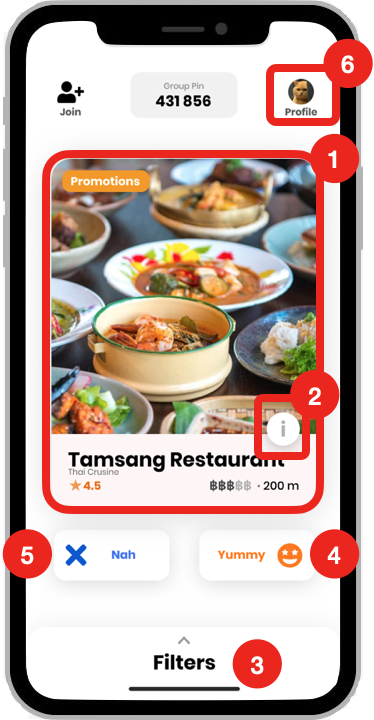
\includegraphics[height=300pt]{./images/3ui_HomePageUserInterfaceDesign.png}
\caption{Home Page User Interface Design}\label{fig:3ui_HomePageUserInterfaceDesign}
\end{figure}\vspace{-24pt}

\begin{enumerate}
\item Restaurant card, it shows the general information about a restaurant.
\item “i” button, when tapped, more information will be shown.
\item Filter button, it will bring up the filter window.
\item Like button, tapped once users are satisfied with the restaurant
\item Dislike button, if users are not satisfied with the restaurant, they can tap this button to see the next suggestion.
\item Profile button, links to the profile page.
\end{enumerate}

After users logged in or registered, they will see the home page. By entering the home page, the system will automatically start recommending some restaurants to users. Users will see the information of each suggested restaurant (1). They can also see some more information about each restaurant by tapping the “i” icon (2). They can filter the suggested restaurants by tapping the “Filters” button (3) and the filter window will appear (Figure~\ref{fig:3ui_FilterWindowUserInterfaceDesign}). If they are satisfied with the suggested restaurant, they can tap on the “Yummy” button (4) or swipe the restaurant card to the right, and then the success page will appear (Figure~\ref{fig:3ui_RecommendationSuccessPageUserInterfaceDesign}). Otherwise, if they are not satisfied with that restaurant, they can tap on the “Nah” button (5) or swipe the restaurant card to the left, and then the system will show the next suggested restaurant to users and let them consider it again. Users can see their profile by tapping the profile picture button (6) and the profile management page will appear (Figure~\ref{fig:3ui_ProfileManagementPageUserInterfaceDesign}).

\newpage
\begin{figure}[H]\centering
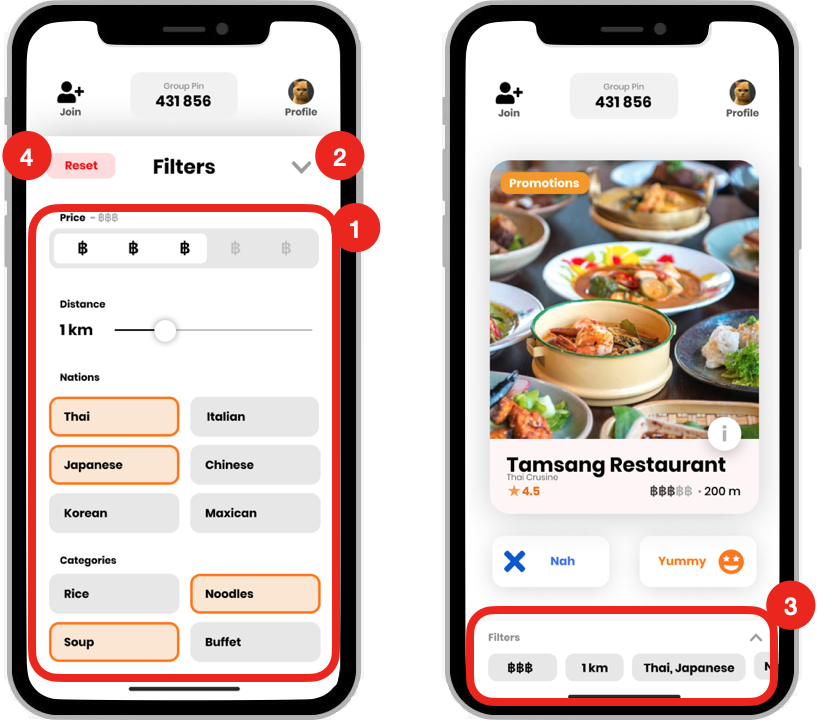
\includegraphics[height=300pt]{./images/3ui_FilterWindowUserInterfaceDesign.png}
\caption{Filter Window User Interface Design}\label{fig:3ui_FilterWindowUserInterfaceDesign}
\end{figure}\vspace{-24pt}

\begin{enumerate}
\item Filtering options.
\item Arrow button, will apply current filtering and close the filter window.
\item Filter button with applied filter tags, users can open the filter window again by tapping this button.
\item Reset button, will remove all the applied filters.
\end{enumerate}

After users tap on the “Filter” button on the home page (number 3 on Figure~\ref{fig:3ui_HomePageUserInterfaceDesign}), the filter window will appear. Users can filter restaurants by choosing the available options that appear on the filter window (1). After finishing choosing the filtering option, they can tap on the arrow icon (2) to apply the filter and the filter window will be minimized. They can see the applied filters at the bottom of the screen (3). They can change their filtering by tapping on the bottom bar (3) to bring the filter window up again. They can tap on the “Reset” button (4) to remove all of the applied filters. After applying any filters, the system will suggest the restaurant that matches its filtering condition.

\newpage
\begin{figure}[H]\centering
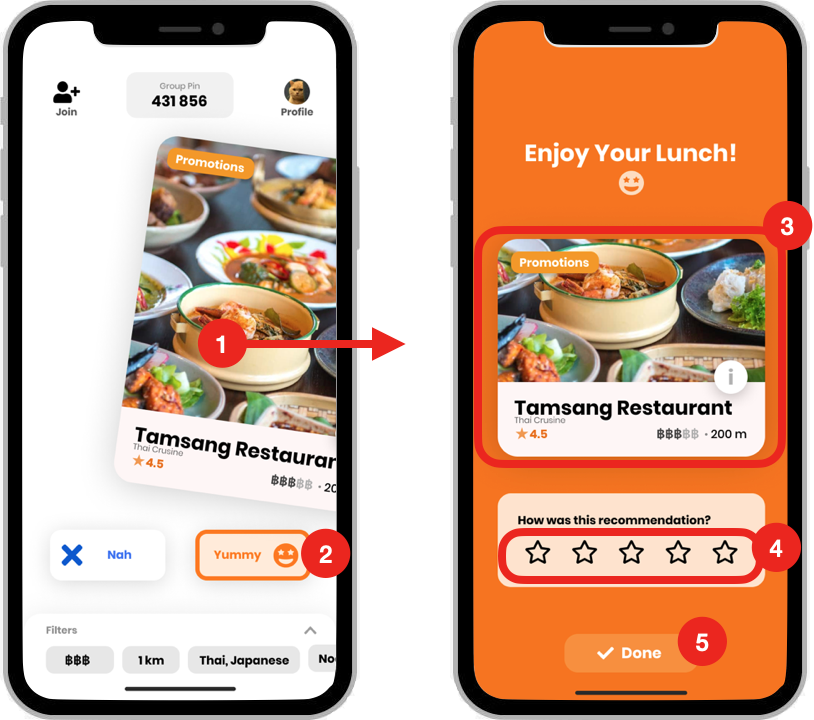
\includegraphics[height=300pt]{./images/3ui_RecommendationSuccessPageUserInterfaceDesign.png}
\caption{Recommendation Success Page User Interface Design}\label{fig:3ui_RecommendationSuccessPageUserInterfaceDesign}
\end{figure}\vspace{-24pt}

\begin{enumerate}
\item Swipe right for the satisfying restaurant.
\item Like button which works the same as the swipe right.
\item Restaurant card showing general information about the liked restaurant.
\item Recommendation rating, let users rate satisfaction with their current recommendation.
\end{enumerate}

On the home page which users see the suggested restaurant, if users are satisfied with the suggested restaurant, they can swipe right (1) or tap on the “Yummy” button (2). After that, the recommendation success page will appear (the right picture in Figure~\ref{fig:3ui_RecommendationSuccessPageUserInterfaceDesign}). On the success page, users can see the restaurant information in the center of the screen (3). They can give a rating score for the recommendation from 1 star to 5 stars (4). After they are done seeing the information, they can tap on the “Done” button (5) to close the success page and they will see the home page (Figure~\ref{fig:3ui_HomePageUserInterfaceDesign}) again.

\newpage
\subsubsection{Group Restaurant Recommendation Page}
\begin{figure}[H]\centering
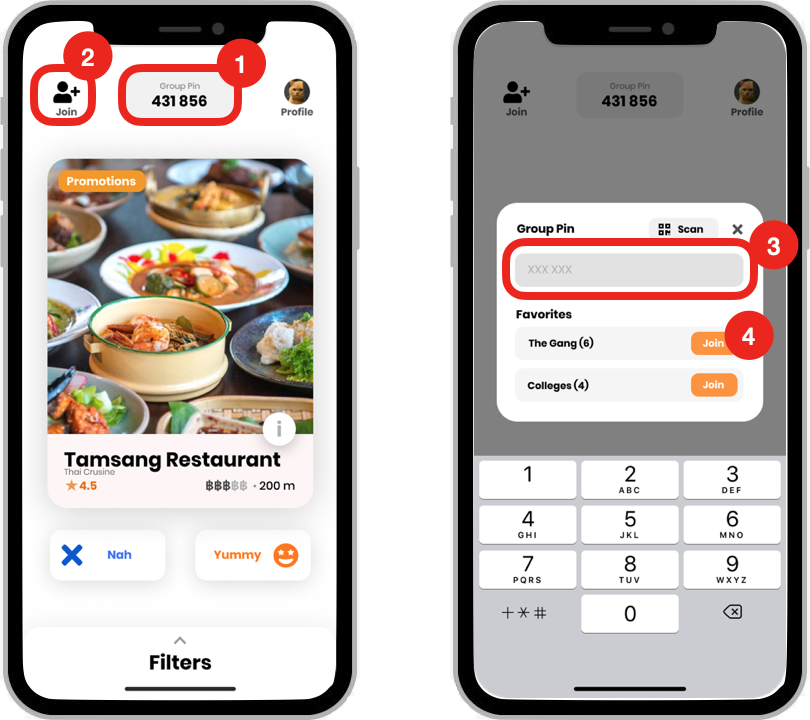
\includegraphics[height=300pt]{./images/3ui_GroupJoiningUserInterfaceDesign.png}
\caption{Group Joining User Interface Design}\label{fig:3ui_GroupJoiningUserInterfaceDesign}
\end{figure}\vspace{-24pt}

\begin{enumerate}
\item Group pin code which other members used for joining the group.
\item Join button, it will bring up the joining dialog
\item Group pin code input field, let users input the group pin code.
\item Join button which lets users join their existing group without input the group pin code again.
\end{enumerate}

In the following section, we will walk through the group recommendation process. On the home page (the left picture in Figure~\ref{fig:3ui_GroupJoiningUserInterfaceDesign}), it will show the group pin on the top of the screen (1). To start the group recommendation, the user has to share this pin code with other members in the group and this will make the pin code owner be the head of the group. Other members can join the group by tapping on the “Join” button (2) and the joining dialog will appear (the right picture in Figure~\ref{fig:3ui_GroupJoiningUserInterfaceDesign}). In the joining dialog, other members can input the pin that appeared on the group head’s device (1). Moreover, users can join the previously joined group, which will be shown as favorites. They can directly join their favorite group by tapping the “Join” button (4) in the group they want to join without input the pin code again. After someone joins the group the group recommendation will be initialized and all members that joined the group will see the group confirmation page next (Figure~\ref{fig:3ui_GroupConfirmationPageUserInterfaceDesign}).

\newpage
\begin{figure}[H]\centering
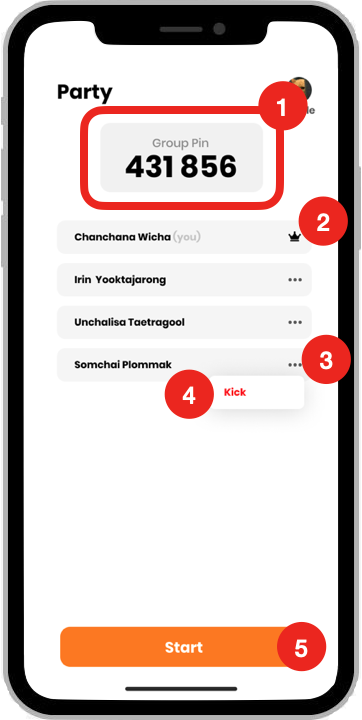
\includegraphics[height=300pt]{./images/3ui_GroupConfirmationPageUserInterfaceDesign.png}
\caption{Group Confirmation Page User Interface Design}\label{fig:3ui_GroupConfirmationPageUserInterfaceDesign}
\end{figure}\vspace{-24pt}

\begin{enumerate}
\item Group pin code which other members used for joining the group.
\item Crown icon indicates who is the head of this group
\item 3 dots icon for more action on each member in the group.
\item Kick button, it let the head remove some members from the group.
\end{enumerate}

After someone joins the group, all joined members will see this group confirmation page. On the top, there is a group pin code that the members in the group can share with other people if they want to join this eating group. The head of the group will have a crown icon (2) and they can manage the members in the group. If the head wants to remove some of the members, they can do it by tapping the 3 dots icon (3) followed by tapping the “Kick” button, after that the kicked member will no longer be in the party. When all members are joined and ready, the head will tap on the “Start” button to begin the group recommendation.

\newpage
\begin{figure}[H]\centering
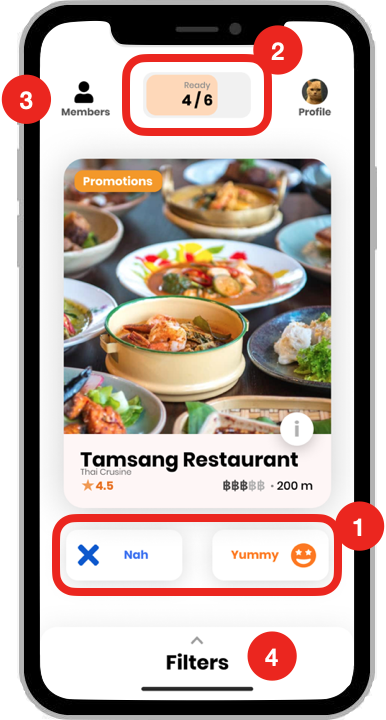
\includegraphics[height=300pt]{./images/3ui_GroupRecommendationPageUserInterfaceDesign.png}
\caption{Group Recommendation Page User Interface Design}\label{fig:3ui_GroupRecommendationPageUserInterfaceDesign}
\end{figure}\vspace{-24pt}

\begin{enumerate}
\item Like or dislike area for choosing the restaurant.
\item Progress bar indicates the progress of the group decision.
\item Members button, will bring up the members dialog which shows all members.
\item Filter button for setting the filters for restaurants.
\end{enumerate}

After the group has been created and confirmed, the group recommendation will begin. All members will see the same suggested set of restaurants. Each member will choose whether they like or not but tapping “Yummy” and “Nah” or swiping (1) is the same as in individual recommendation. The group recommendation will be finished after all members like the same restaurant. The top bar (2) indicates the highest number of members that agree on the same restaurant, when it is full, it means everybody agrees on the same restaurant and the recommendation is finished. Users can see the members by tapping the “Member” button (3). Users still can set the filter by tapping the “Filter” button (4) but this time the filters will be applied to every member in the group.

\newpage
\subsubsection{Profile Page}
\begin{figure}[H]\centering
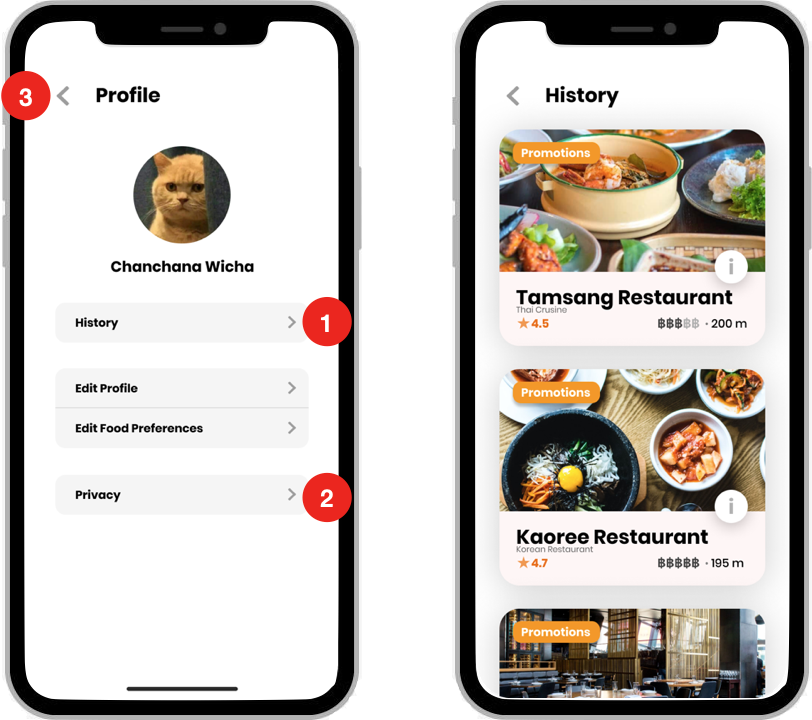
\includegraphics[height=300pt]{./images/3ui_ProfileManagementPageUserInterfaceDesign.png}
\caption{Profile Management Page User Interface Design}\label{fig:3ui_ProfileManagementPageUserInterfaceDesign}
\end{figure}\vspace{-24pt}

\begin{enumerate}
\item History button, it links to the history page (the right picture in Figure~\ref{fig:3ui_ProfileManagementPageUserInterfaceDesign})
\item Privacy button, it let users change their password and their privacy setting.
\item Back button which brings users back to their home page.
\end{enumerate}

After users choose to view their profile (number 6 in Figure~\ref{fig:3ui_HomePageUserInterfaceDesign}), they will see the left picture in Figure~\ref{fig:3ui_ProfileManagementPageUserInterfaceDesign}. They can choose to view their selected restaurant history by tapping the “History” button (1) and a list of selected restaurants will be shown (the right picture of Figure~\ref{fig:3ui_ProfileManagementPageUserInterfaceDesign}). They can also choose to edit their profile such as their name, gender, or birthdate or choose to edit their food preferences. They can reset their password and set the privacy setting under the “Privacy” section (2). They can go back to the main screen by tapping the arrow icon (3).


\section{Database Structure} \label{sec:databasestructure}
In this section, we explain our database structure in the \textit{Database} component. Our database stores all information for our system as a NoSQL database. Then, we discuss the database collection’s name and description, the schema of each collection, and database indexing.

\newpage
\subsection{Collections}
\begin{table}[H]
\caption{Database Collection and Description}\label{tbl:3DatabaseCollectionandDescription}
\begin{tabularx}{\textwidth}{l|X} \hline\hline
Collection Name & Description \\ \hline\hline
restaurants & Restaurant information including name, address, photo URL, etc., restaurant profile. \\ \hline
users & User information including authentication information, general information such as name, gender, age, and food preference information. \\ \hline
recommendations & Information for each recommendation session. This collection includes all of the interaction histories from the user in each recommendation session. \\ \hline
categories & Information about restaurant categories. We keep the categories separated with restaurant collection to reduce the redundancy. \\ \hline
favorites & Keep the information about the favorite list of restaurants for each user. \\ \hline\hline
\end{tabularx}
\end{table}

Table~\ref{tbl:3DatabaseCollectionandDescription} shows us all collections in our NoSQL database, their collection’s name, and their description. Our database contains mainly 5 collections including restaurants, users, recommendations, categories, and favorites.

\subsection{Schema}

Although NoSQL does not have a fixed database schema, by using Mongoose as a MongoDB database connection framework, it provides some primary schema for data creating and reading facilitation. Having Mongoose’s schema can help us manage a uniform data format with easy schema migration. However, inserting data with a different format from Mongoose’s schema does not break the process and no part of the data will be discarded. In this section, we will show some mandatory fields for each collection.


\begin{table}[H]
\caption{Restaurant Schema}\label{tbl:3RestaurantSchema}
\begin{tabularx}{\textwidth}{l|l|X} \hline\hline
Key Name & Type & Description \\ \hline\hline
name & String & Name of the restaurant \\ \hline
profile.categories & Array of ObjectId & Restaurant categories such as Thai, Korean, Fast Food. This field references category collection using their category id. \\ \hline
profile.price\_range & Number & The price range of the restaurant, from 1-4. \\ \hline
profile.rating & Number & Facebook users’ rating of the restaurant. From 1 to 5 stars. \\ \hline
profile.likes & Number & The number of users that liked the restaurant’s Facebook page. \\ \hline
address & String & One line address string of the restaurant. \\ \hline
location.coordinates & Array of Numbers & Coordinate of the restaurant in form of [longitude, latitude] \\ \hline
link & String & URL link to their Facebook page. \\ \hline\hline
\end{tabularx}
\end{table}

\begin{table}[H]
\caption{User Schema}\label{tbl:3UserSchema}
\begin{tabularx}{\textwidth}{l|l|X} \hline\hline
Key Name & Type & Description \\ \hline\hline
authentication & Object & Authentication token object for user login. \\ \hline
username & String & Username of the user. \\ \hline
password & String & Encrypted password of the user. \\ \hline
profile.gender & String & Gender of the user. \\ \hline
profile.birthdate & Date & Birthdate of the user. \\ \hline
profile.preference & Object & Food preferences of users. \\ \hline\hline
\end{tabularx}
\end{table}

\begin{table}[H]
\caption{Recommendation Schema}\label{tbl:3RecommendationSchema}
\begin{tabularx}{\textwidth}{l|l|X} \hline\hline
Key Name & Type & Description \\ \hline\hline
users & Array of ObjectId & Users that request the recommendation. This field references user collection using their user id. \\ \hline
histories & Array of Object & User interaction history in each recommendation session. \\ \hline
histories.restaurant & ObjectId & Interacted restaurant. This field references restaurant collection using their restaurant id. \\ \hline
histories.is\_love & Boolean & Whether users select go or not go to the interacted restaurant. \\ \hline
histories.timestamp & Date & The timestamp of each interaction history. \\ \hline
location.coordinate & Array of Numbers & The location that this recommendation session occurs in the form of [longitude, latitude]. \\ \hline\hline
\end{tabularx}
\end{table}

\begin{table}[H]
\caption{Category Schema}\label{tbl:3CategorySchema}
\begin{tabularx}{\textwidth}{l|l|X} \hline\hline
Key Name & Type & Description \\ \hline\hline
name & String & Name of the category eg. Thai Restaurant, Korean Restaurant, or Fast Food Restaurant. \\ \hline
is\_common & Boolean & Whether this category is a common category. \\ \hline\hline
\end{tabularx}
\end{table}

\begin{table}[H]
\caption{Favorite Schema}\label{tbl:3FavoriteSchema}
\begin{tabularx}{\textwidth}{l|l|X} \hline\hline
Key Name & Type & Description \\ \hline\hline
user & ObjectId & User of the current record. \\ \hline
restaurants & Array of & List of their favorite restaurants. \\ \hline\hline
\end{tabularx}
\end{table}

Note that we need to keep a category collection separated from restaurant information because some of the collected restaurant data may have a different name but same id or different id with the same name so we want to keep this information correctly and easily maintained later.


\subsection{Indexing}

With database indexing, we can query the data faster by storing additional information about data. Every collection has an indexed id so that we can query the data from their id faster. However, we also set more indexing on 2 collections which are restaurants and users.

\begin{figure}[H]\centering
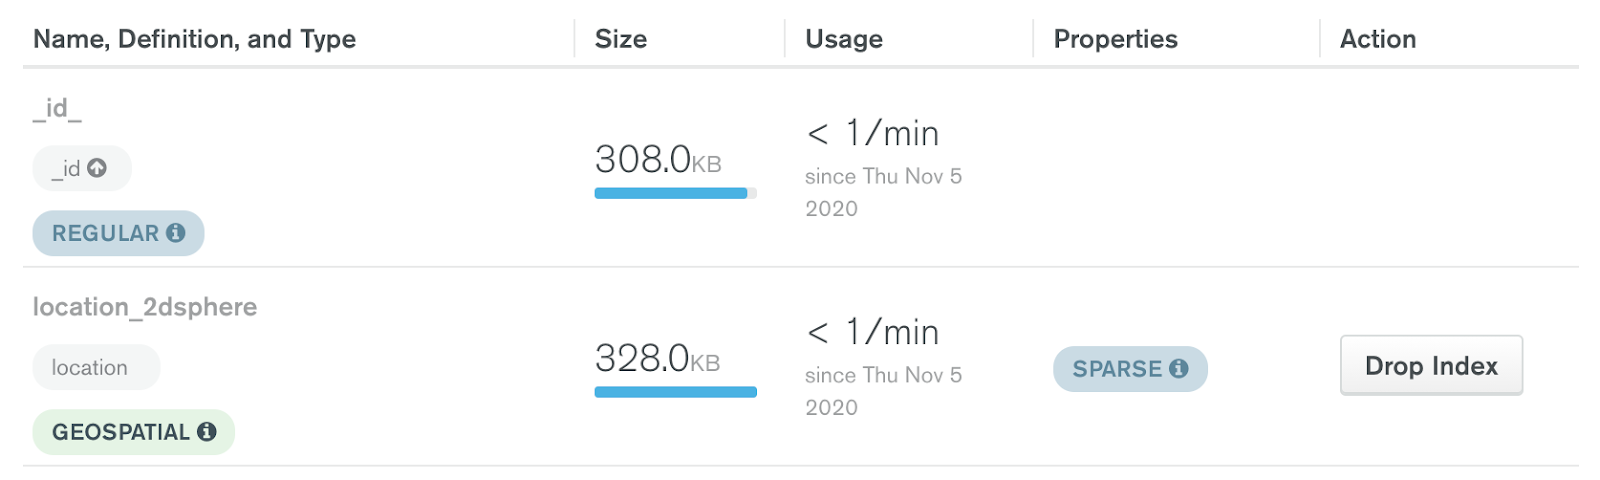
\includegraphics[width=400pt]{./images/3db_RestaurantCollectionsIndexes.png}
\caption{Restaurant Collection’s Indexes}\label{fig:3db_RestaurantCollectionsIndexes}
\end{figure}\vspace{-24pt}

From Figure~\ref{fig:3db_RestaurantCollectionsIndexes}, we can see that the restaurant collection has one more index which is the location index. This index is used for query restaurants by a distance of 2 coordinates.
\begin{figure}[H]\centering
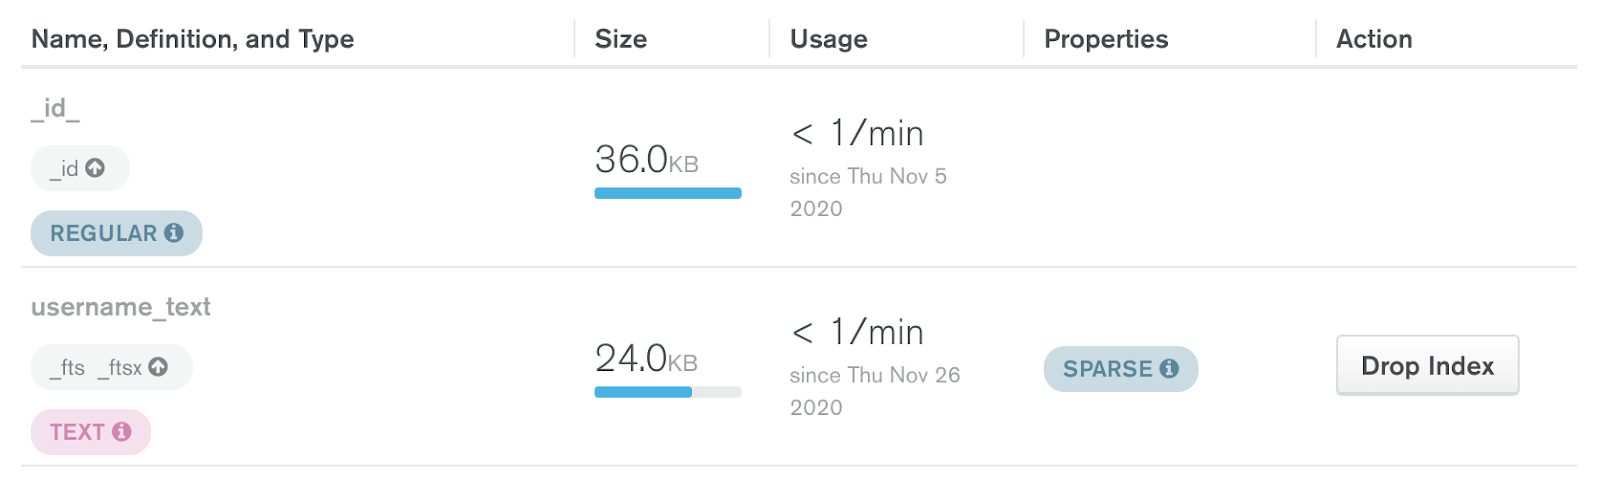
\includegraphics[width=400pt]{./images/3db_UserCollectionsIndexes.png}
\caption{User Collection’s Indexes}\label{fig:3db_UserCollectionsIndexes}
\end{figure}\vspace{-24pt}

From Figure~\ref{fig:3db_UserCollectionsIndexes}, we can see that the user collection has one more index which is the username index. This index is used for query users by username. It also helps when checking the username’s availability. The username index also applies to other collections that require finding  the record by the username which is the favorite collection.


\section{Restaurant Recommendation Algorithm}

Since last semester, our first try was to use a user-based collaborative filtering technique for the individual’s recommendation system. The result was quite good but not enough for our objective due to its limitations which are the cold-start and location-based problem. Moreover, this technique only works with individual recommendation. So, we decided to research other recommendation techniques in order to reach the objective faster and less complicated than the collaborative filtering techniques.

In conclusion, we decided to use the \textit{\textbf{Genetic Algorithm}} for our restaurant recommendation system which is able to apply to both individuals and groups by creating an objective function to maximize the user’s satisfaction.

\newpage
\subsection{Genetic Algorithm for Individual Recommendation}

\begin{figure}[H]\centering
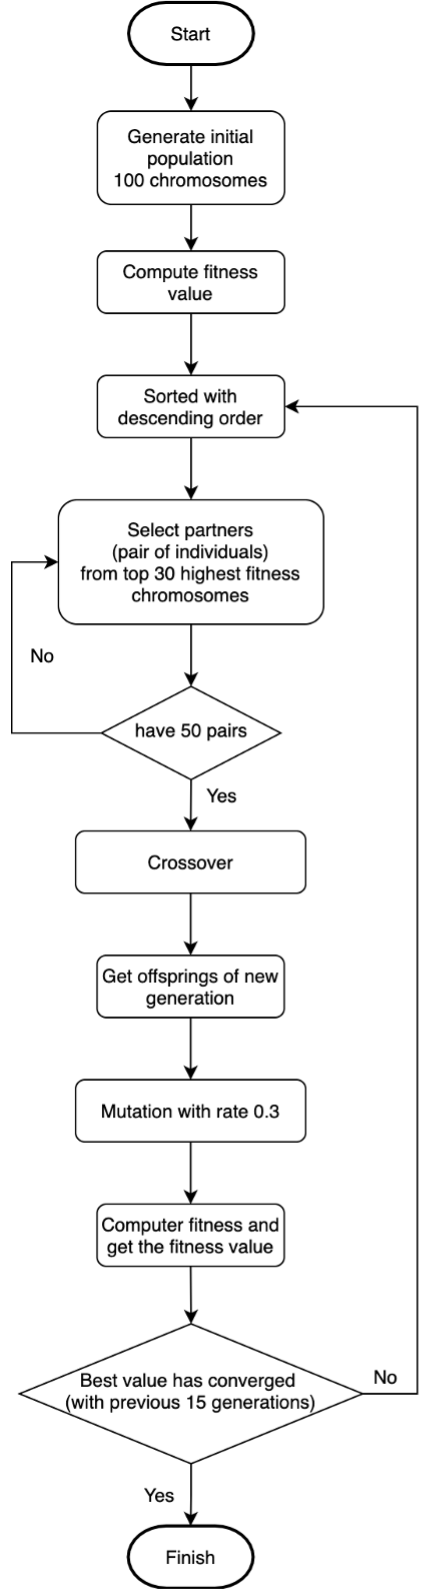
\includegraphics[height=600pt]{./images/3GeneticAlgorithmFlowchart.png}
\caption{Restaurant Recommendation Process for Individual}\label{fig:3GeneticAlgorithmFlowchart}
\end{figure}\vspace{-24pt}

Figure~\ref{fig:3GeneticAlgorithmFlowchart} displays the main process of the restaurant recommendation by applying the principles of the Genetic Algorithm to the system.

\textbf{1. Initial Population}\par

One set of the restaurant recommendations consists of 10 restaurants. In the genetic algorithm, one chromosome then contains 10 genes for 10 restaurants.  Initially, restaurants are drawn from the database based on the user's surroundings or selected locations only. Then, the restaurants are randomly assigned to each gene in the chromosome. Figure~\ref{fig:3ga_init} shows the example of the genes in one chromosome that has a list of restaurants R1 to R10. We set the number of chromosomes to 100. Therefore, 100 chromosomes are initialized in the same manner.

\begin{figure}[H]\centering

\includegraphics[width=300pt]{./images/3ga_init.png}
\caption{Example of Population in 1 Chromosome}\label{fig:3ga_init}
\end{figure}\vspace{-24pt}

\textbf{2. Selection}\par

The proper selection of genes will have a selection process through objective function or fitness function. Our system wants to maximize the users’ satisfaction based on their preferences and interests. Therefore, we have formulated the equation of our objective function as follows:

\begin{equation}\label{eq:maximizes}
maximize S = \sum_{i=1}^{10}(T_i + C_i + F_i)
\end{equation}

\begin{blockquote}\leftskip=8em
\textbf{Given}\\
$S$; Value of user’s satisfaction\\
$i$; Each restaurant in 1 chromosome (Gene Position)\\
$T_i$; A score of the restaurant type that meet user’s preferences\\
$C_i$; A score of the price range that meet user’s preferences\\
$F_i$; A score  the restaurant that meet the user’s history selection

\end{blockquote}


\begin{blockquote}
\textbf{With condition}
\vspace{-12pt}
\begin{itemize}\leftskip=2em
\item[-] $S \geq 0$; The user’s satisfaction value must be greater than or equal to zero.
\item[-] $T_i=0, 1, 2, \cdots, 15$; The score is based on user rankings from the preferences page by the first place equals five points and decreases accordingly where one restaurant can have a maximum of five categories, so the possible largest number of this variable is $5 + 4 + 3 + 2 + 1 = 15$.
\item[-] $C_i=0,1,2,3,4$; The score is based on the user’s price range interest. If a restaurant price range matches with the user’s interest, it will get four points and decrease when the restaurant price range is less than the user's interest. If the restaurant price ranges greater than the user's interest, it will be all zero.
\item[-] $F_i=0$; The score is based on the user’s history of restaurant selection. If the restaurant matches the user’s selection, it will get one point. If the restaurant doesn’t match, it will be equal to zero.
\end{itemize}
\end{blockquote}

After the system computes all fitness values, the chromosomes will be sorted in descending order and then select individuals from the top 30 to be parents to reproduce the next generation.

\textbf{3. Reproduction}\par

From the top 30 chromosomes, the system randomly matches the pair until it reaches 50 pairs. After that the crossover and mutation methods are performed in order to generate a new population with better quality and more diversity from the previous generation.

In the crossover method, the developers wanted to recommend a unique restaurant all in one set of recommendations. Thus, a method of crossover executes one gene at a time with a 70\% chance of crossover. If the crossover has occurred and the restaurant is repeated, the system will skip that gene immediately.

In the mutation method, the developers have set the number of chances that a chromosome in each generation will mutate to 30\%. The mutation process is performed by randomly recruiting a new restaurant from the database to provide more variety than the previous generation.

\textbf{4. Termination}\par

The algorithm will be terminated when the fitness values of 15 generations are all the same which implies that the algorithm cannot find a better generation that has a higher fitness value.

\subsection{Genetic Algorithm for Group Recommendation}

\begin{figure}[H]\centering
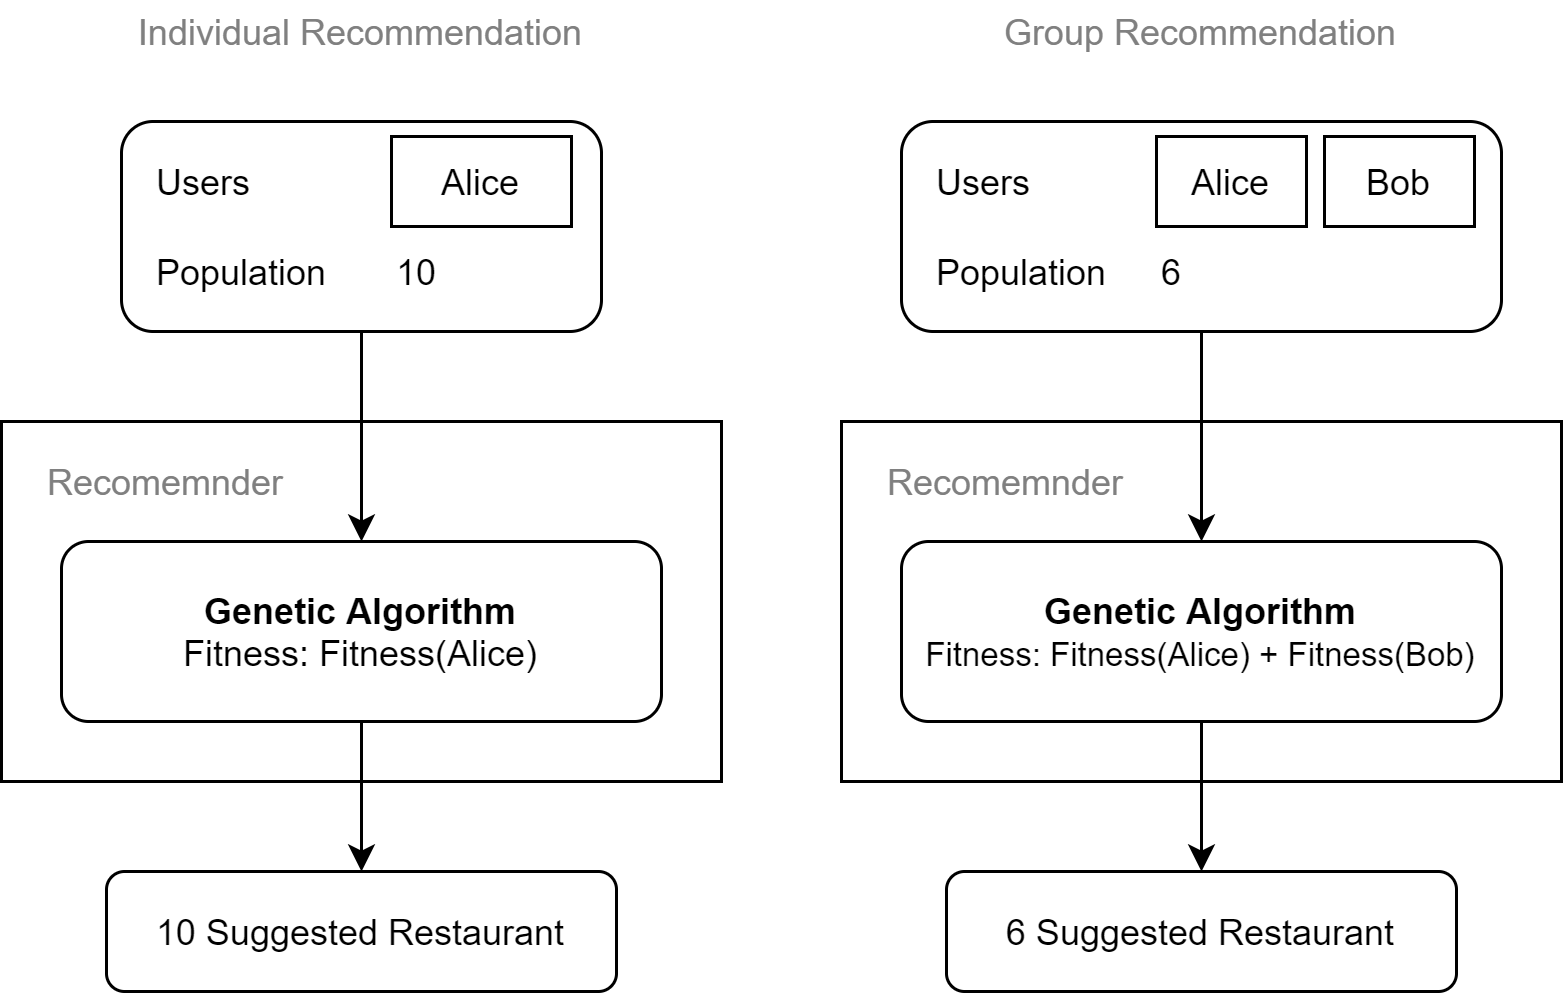
\includegraphics[width=300pt]{./images/3ga_grouprecflow.png}
\caption{Group Recommendation Flow}\label{fig:3ga_grouprecflow}
\end{figure}\vspace{-24pt}

For the group recommendation, the same process as individual recommendation is conducted. However in the group recommendation, the system suggests the restaurant in a set of six instead of ten. So, we need to change the number of genes in one chromosome from ten to six. Moreover, the group recommendation will bring each user’s maximum satisfaction value and aggregate to be the final solution of the group.

\subsection{Rank Aggregation for Group Recommendation}

%TODO check for update

\begin{figure}[H]\centering
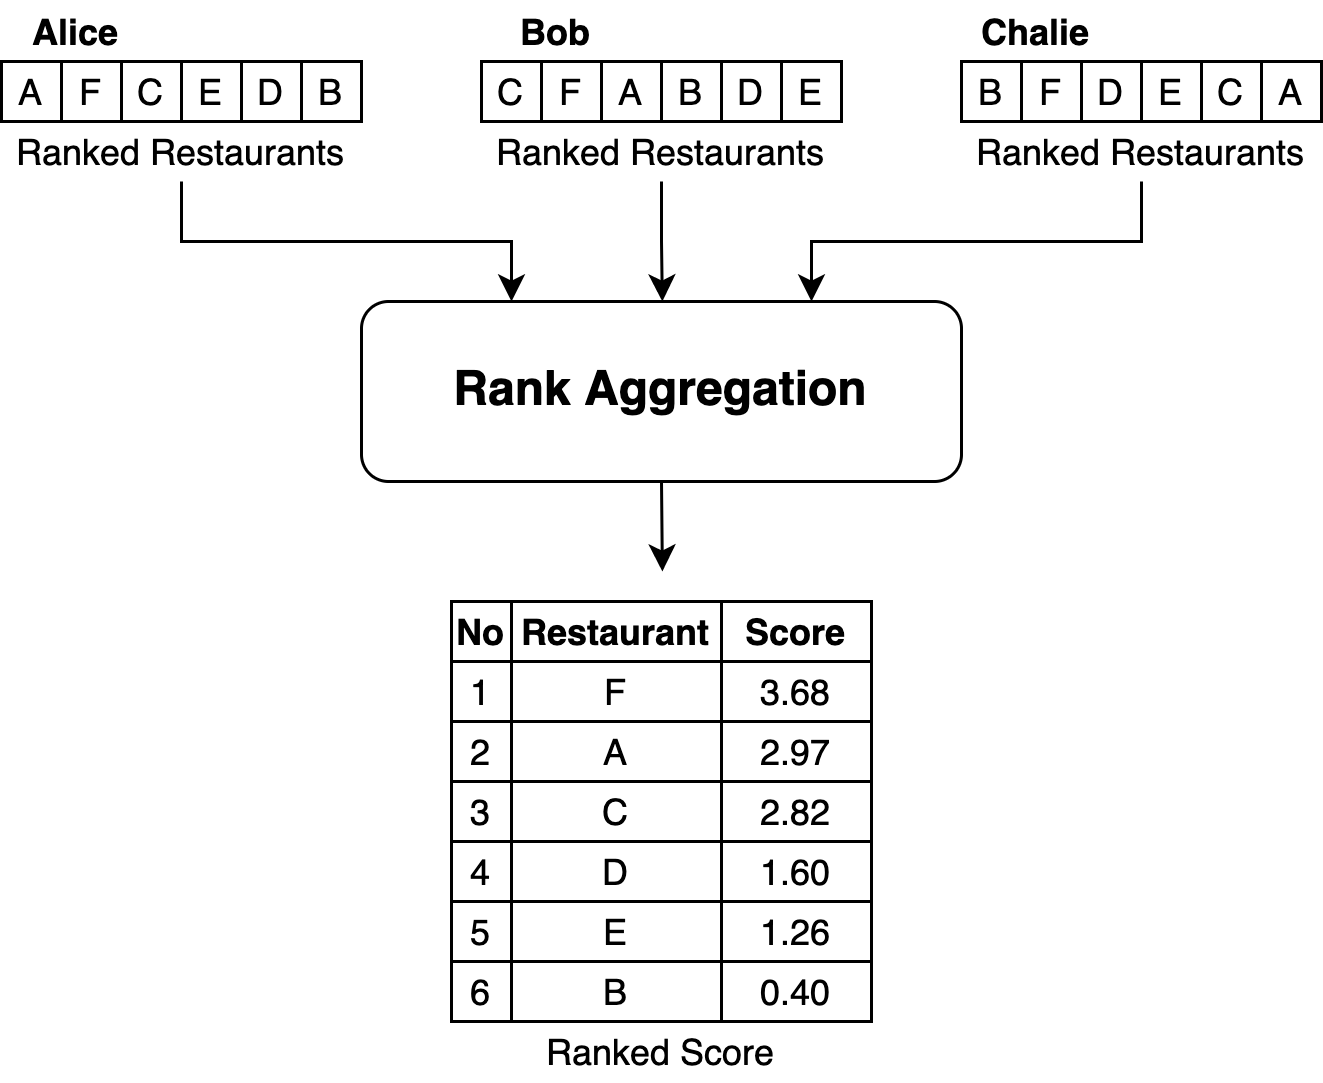
\includegraphics[width=300pt]{./images/3ga_rankagg.png}
\caption{Rank Aggregation}\label{fig:3ga_rankagg}
\end{figure}\vspace{-24pt}

Rank Aggregation is a process that finalizes the suggested restaurants from every members’ ranked restaurants. Firstly, it gathers all ranked restaurants from all members. Then, it calculates the score for each restaurant based on the formula below. The higher score means that the restaurant is more suitable for the group. Therefore, the restaurant with the highest score is considered to be the final restaurant for the group.

\begin{equation}\label{eq:rankaggscore}
score = \left (\frac{T}{T_{max}}  \right ) + 2\cdot \left (\frac{R}{R_{max}}  \right ) + \left (\frac{C}{C_{max}}  \right )
\end{equation}
\begin{equation}\label{eq:rankaggscorerank}
R = \sum_{i=1}^{n}r - \sqrt{\sum_{\substack{j=1 \\ j\neq k}}^{n}\sum_{k=1}^{n}(r_j - r_k)^2}
\end{equation}

\begin{blockquote}\leftskip=8em
\textbf{Given}\\
$T$; Restaurant type score\\
$T_{max}$; Maximum restaurant type score of the set\\
$R$; Rank score\\
$R_{max}$; Maximum rank score of the set\\
$C$; Restaurant cost score\\
$C_{max}$; Maximum restaurant cost score of the set\\
$r$; Rank score from each member, score from 1 - 6
\end{blockquote}

The score of each restaurant is calculated using the formula~\ref{eq:rankaggscore} based on 3 factors: restaurant’s category type, rank from users and restaurant’s cost. The type and cost scores of each restaurant can be derived from the user’s preference. genetic algorithm’s fitness value calculation process. The rank score from each member $r$ is determined by the position of the restaurant of the member.  The first rank restaurant receives a score of 6, the second receives a score of 5, and so on until the last rank receives a score of 1. Then, these rank scores are summed up to be rank score $R$. However, we need to subtract how far each restaurant ranked from each member in order for the final score to be more fair for all members. 

For example, Alice ranked the top three restaurants as A, F, and C, while Bob ranked them C, F, and A. The score of restaurant A is $10$, from $6 + 4$, and the score of restaurant B is also $10$, from $5 + 5$. This example demonstrates that even if Bob placed restaurant A on his third rank, it does not matter because the score is dominated by Alice's ranking score. So, by subtracting the rank score of restaurant A, which is $10$, with how far each restaurant ranked which in this case is $2$, from $\sqrt{(6-2^2)}$, the final rank score of restaurant A will be $8$ which is more fair to Bob and the restaurant B still gets a score of $10$, from $10-\sqrt{(5-5^2)}$.

Lastly, the type score, rank score and cost score, are normalized with min-max normalization, so that the scores are all between 0 and 1. However, we multiply the normalized rank score with 2 because this score needs to be dominant with how each member ranks the restaurants over the restaurant profile score. Thus, the restaurant score obtained from this algorithm is a range from 0 to 4.

\section{Production Testing Plan}

\subsection{Production Deployment}

We will deploy our components that need to listen to requests and send requests to other components which are \textit{App Client}, \textit{App Server}, \textit{Recommender}, and \textit{Database}. \textit{App Client}, \textit{App Server}, and \textit{Recommender} will be deployed on Google Cloud App Engine since the deployment service is flexible for multiple programming languages and supports auto scalability. \textit{Database} will be deployed on MongoDB Atlas which is an official cloud deployment service for MongoDB databases. Both Google Cloud App Engine and MongoDB Atlas provide an interactive dashboard for monitoring the performance.

\subsection{User Evaluation}

We will test our application and gather feedback from 20 people. We will collect the data about overall satisfaction, usability, user experience, and improvement suggestions. After the data has been collected, we will analyze and evaluate the application.

\subsection{Application Evaluation}

The performance of main components, \textit{App Client}, \textit{App Server}, and \textit{Recommender}, will be evaluated by monitoring the response latency and doing load tests. The production application performance metrics can also be retrieved by the Google Cloud App Engine dashboard.


%%%%%%%%%%%%%%%%%%%%%%%%%%%%%%%%%%%%%%%%%%%%%%%%%%%%%%%%%%%%%%%%%%%%%%%%%%%
%%%%%%%%%%%%%%%%%%%%%%%%%%%%%%%%%%%%%%%%%%%%%%%%%%%%%%%%%%%%%%%%%%%%%%%%%%%
%%%%%%%%%%%%%%%%%%%%%%%%%%%%%%%%%%%%%%%%%%%%%%%%%%%%%%%%%%%%%%%%%%%%%%%%%%%
%%%%%%%%%%%%%%%%%%%%%%%%%%%%%%%%%%%%%%%%%%%%%%%%%%%%%%%%%%%%%%%%%%%%%%%%%%%
%%%%%%%%%%%%%%%%%%%%%%%%%%%%%%%%%%%%%%%%%%%%%%%%%%%%%%%%%%%%%%%%%%%%%%%%%%%
\chapter{Results and Discussion}

\section{Restaurant Data Collection}

\subsection{Collection Process}


Our system needs to recommend restaurants to users, so restaurant data is crucial data for our system. First, we obtained general restaurant information from the Thai Chana platform via their API endpoint, ‘https://api-search.thaichana.com/’, that information includes the name and coordinates of restaurants.

\begin{figure}[H]\centering
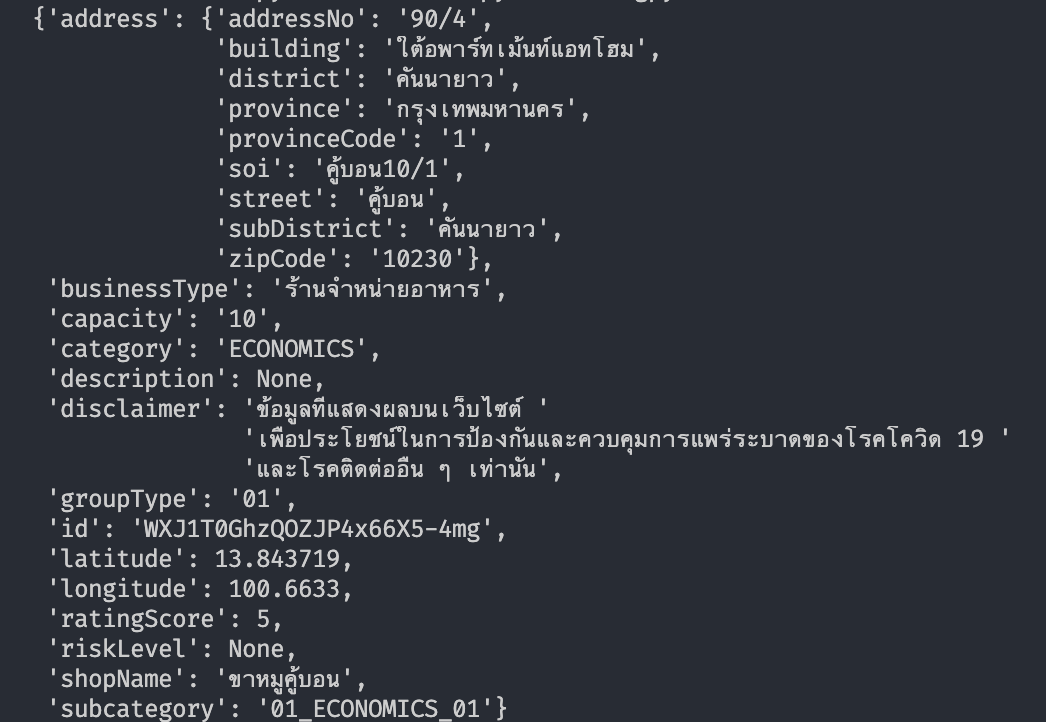
\includegraphics[width=400pt]{./images/4ThaiChanasRestaurantDataExample.png}
\caption{Thai Chana’s Restaurant Data Example}\label{fig:4ThaiChanasRestaurantDataExample}
\end{figure}\vspace{-24pt}

Figure~\ref{fig:4ThaiChanasRestaurantDataExample} shows an example of Thai Chana’s restaurant data. However, there is one issue with this data which is it does not contain information about the categories of restaurants which we need to use in the data analytic and machine learning part. To overcome this issue, we will use Facebook Graph API for additional information. We used names of restaurants from Thai Chana data to query new restaurant information from Facebook Graph API which contains tags about restaurant categories.

\newpage
\begin{figure}[H]\centering
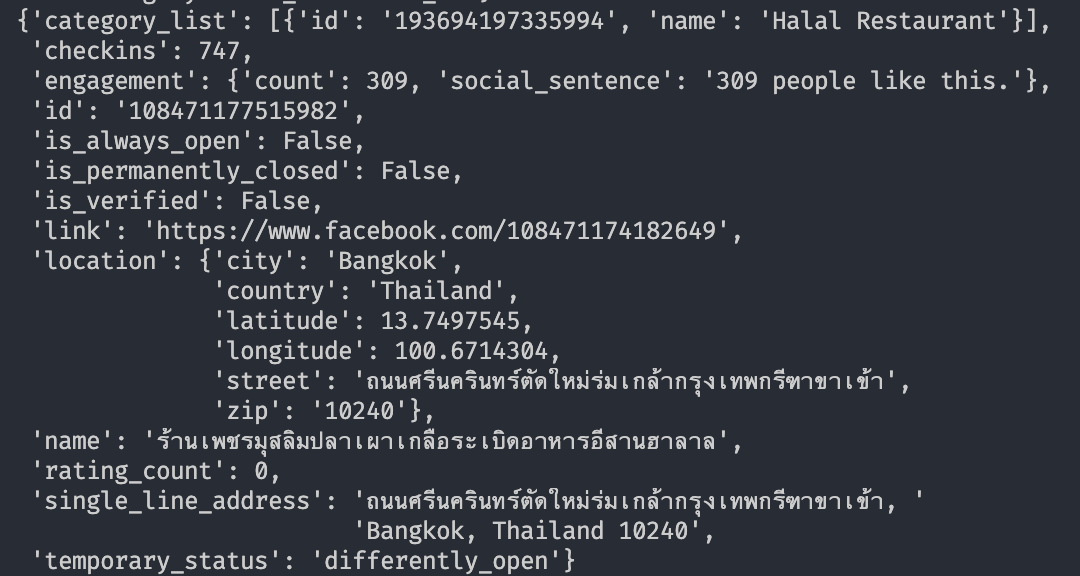
\includegraphics[width=400pt]{./images/4FacebooksRestaurantDataExample.png}
\caption{Facebook’s Restaurant Data Example}\label{fig:4FacebooksRestaurantDataExample}
\end{figure}\vspace{-24pt}

Figure~\ref{fig:4FacebooksRestaurantDataExample} shows an example of Facebook Graph API data. The data contains all information we need such as name, coordinate and restaurant profile such as restaurant categories, price range, and engagement. Moreover, some restaurant data contains image URLs for the restaurant which is very useful for users’ consideration.

\subsection{Preprocessing Process}

For restaurant data preprocessing, it consists of mainly 2 processes which are data transforming and restaurant duplication checking.

In data transformation, we format our collected data into the right format from our database schema. This transformation process happens in the \textit{Data Service} component and then it will send each restaurant to \textit{App Server}. Consequently, \textit{App Server} has a logic for solving restaurant duplication problems that we have faced. This issue is very common because some restaurants may create multiple Facebook pages. So, Facebook data did not guarantee that all of the restaurants in the data is unique. To fix this problem, \textit{App Server} detects the duplicated restaurant.

\newpage
\begin{figure}[H]\centering
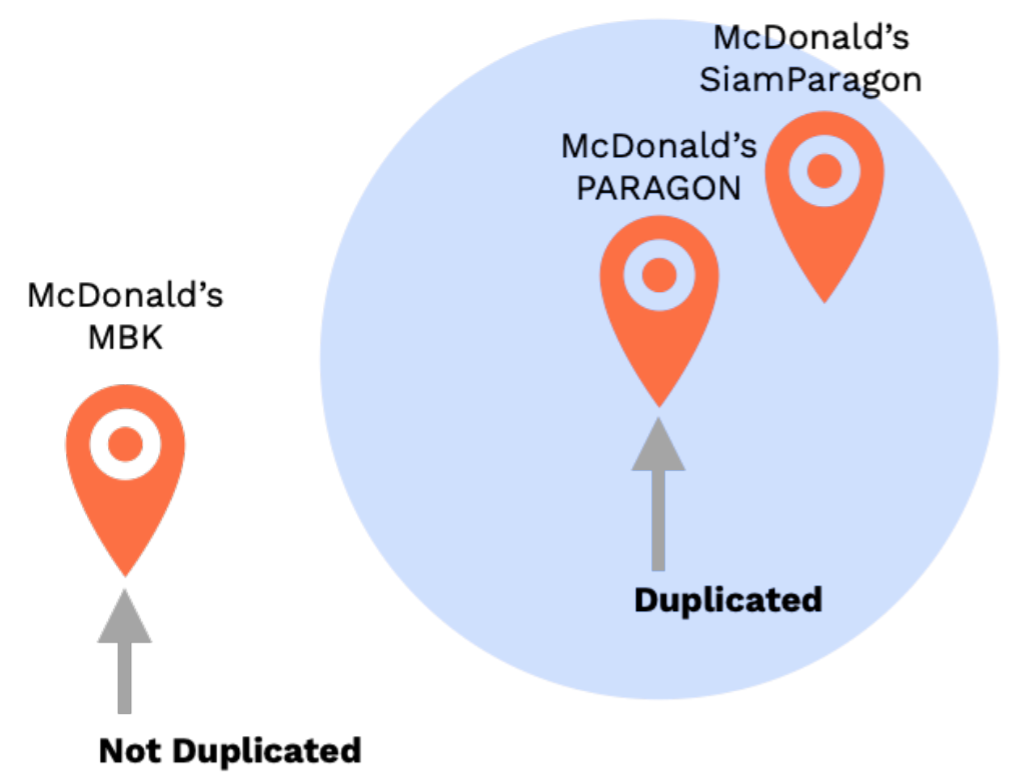
\includegraphics[width=250pt]{./images/4RestaurantDuplicationChecking.png}
\caption{Restaurant Duplication Checking}\label{fig:4RestaurantDuplicationChecking}
\end{figure}\vspace{-24pt}

The restaurant duplication checking is done by checking their name’s similarity with a ratio of 0.65 and their distance from the new incoming restaurant with all of the existing restaurants in the 200 meters range from our database. The system will choose to store only the restaurant that contains more information.

Figure~\ref{fig:4RestaurantDuplicationChecking} shows an example of restaurant duplication checking. We can see that “McDonald’s PARAGON” and “McDonald’s SiamParagon” are very close to each other and the name similarity is more than our threshold. Therefore, the system will classify one of the restaurants as a duplicate and choose to store only one that contains more information. However, “McDonald’s MBK” has a similar name with “McDonald’s PARAGON” but it is not in the range of 200 meters. The system then will not detect this restaurant as a duplicate, which is correct because it is a different branch.

\subsection{Result}

After the restaurant data has been collected, transformed, and cleaned, we got a total of 11,175 restaurants over Bangkok. The visualization of the restaurant data will be described in the following section.

\begin{figure}[H]\centering
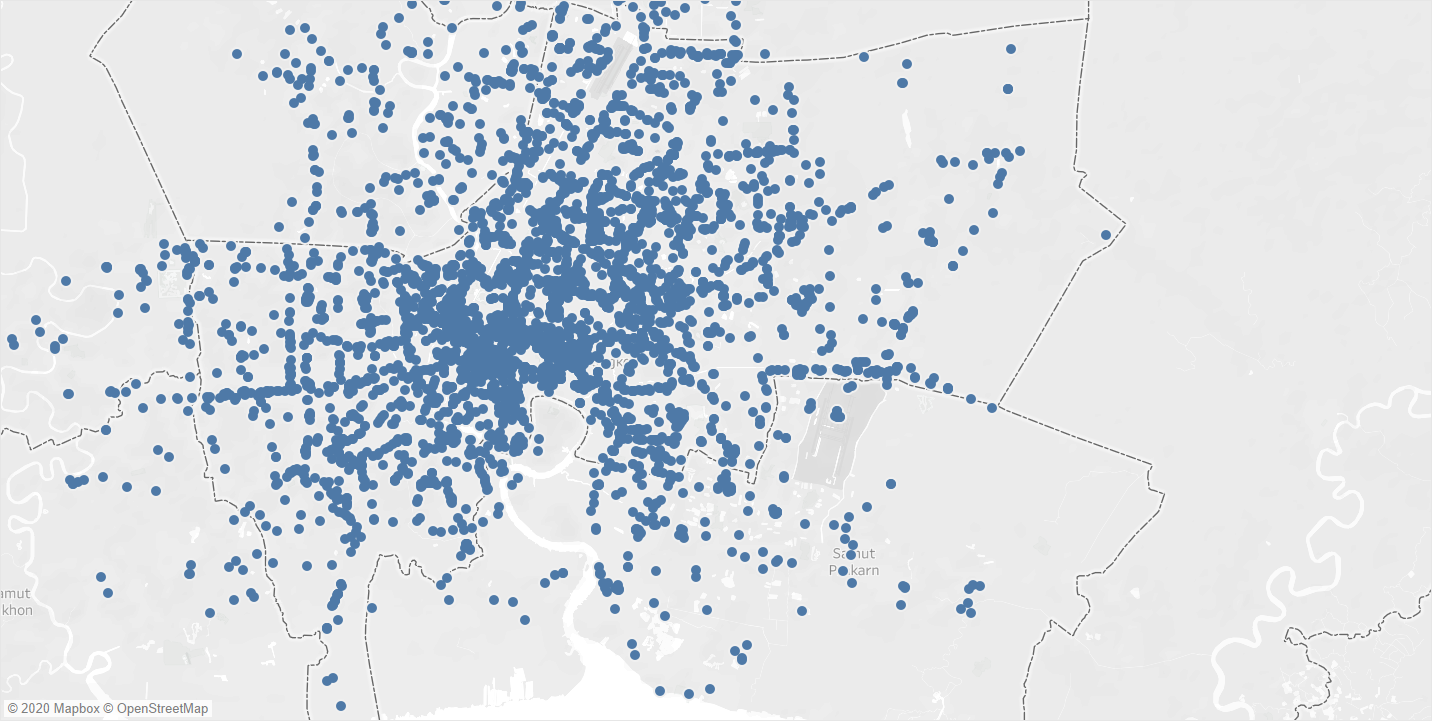
\includegraphics[width=250pt]{./images/4RestaurantsLocationinMap.png}
\caption{Restaurant’s Location in Map}\label{fig:4RestaurantsLocationinMap}
\end{figure}\vspace{-24pt}

Figure~\ref{fig:4RestaurantsLocationinMap} illustrates the distribution of the restaurant’s locations in our data. The data contains restaurants distributed around Bangkok and spread a little bit to the perimeters. Most of the restaurants are located in the center of Bangkok.

\begin{figure}[H]\centering
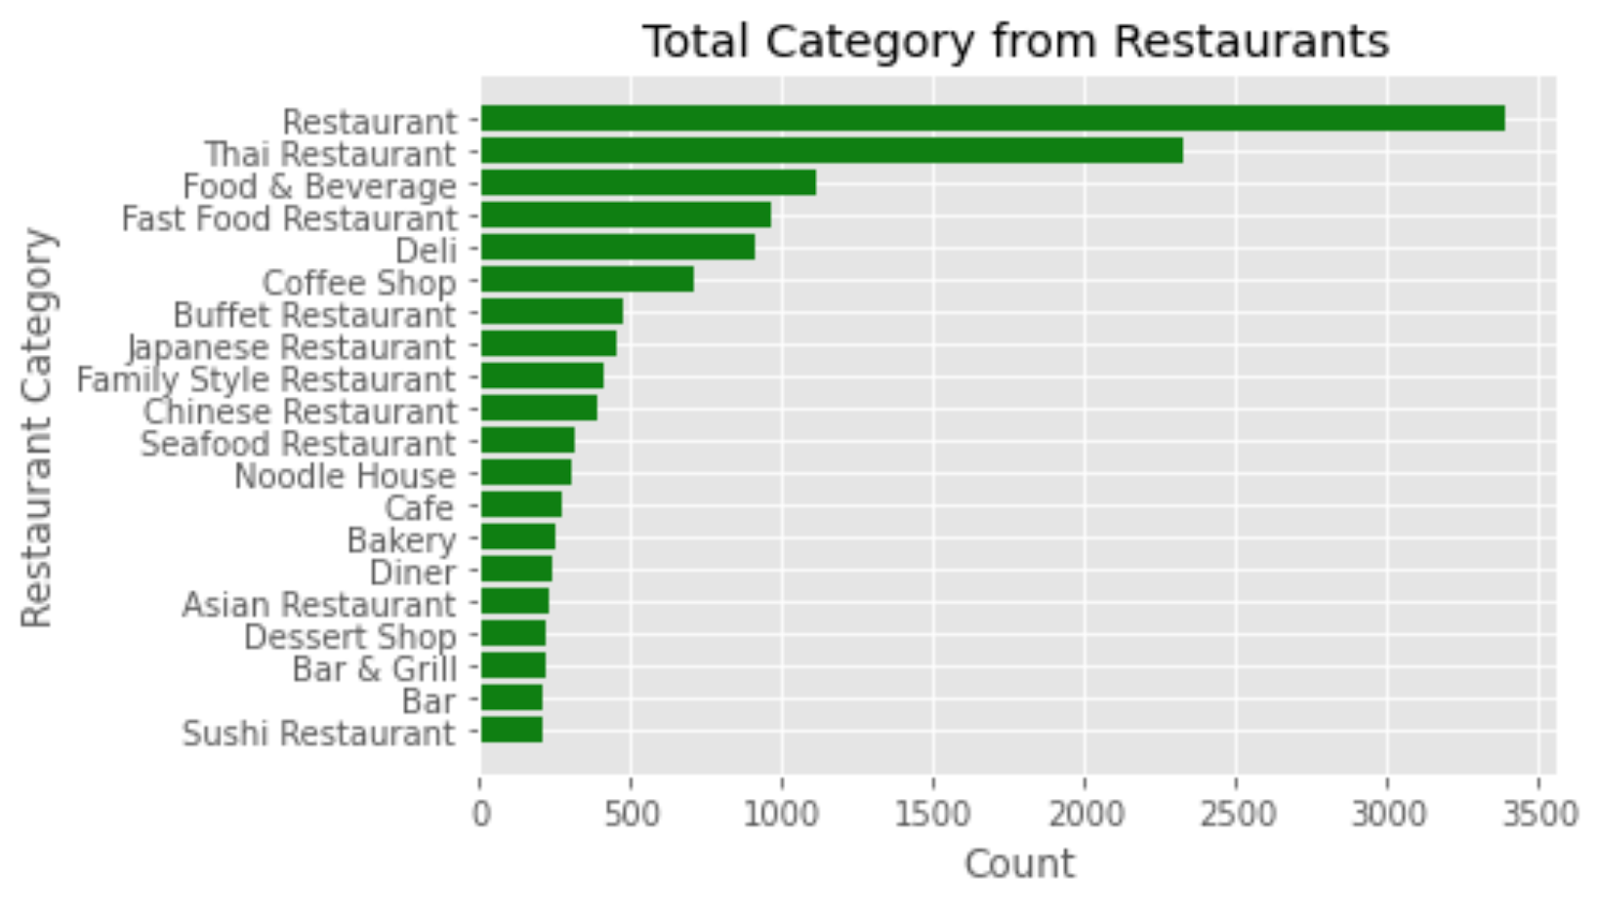
\includegraphics[width=350pt]{./images/4RestaurantsCategoryDistribution.png}
\caption{Restaurant’s Category Distribution}\label{fig:4RestaurantsCategoryDistribution}
\end{figure}\vspace{-24pt}

Figure~\ref{fig:4RestaurantsCategoryDistribution} shows the distribution of the restaurant category in our data. The top restaurant categories are Restaurant, Thai Restaurant, Food \& Beverage, and Fast Food Restaurant. However, we cannot use the tag Restaurant because it does not give any information about the restaurant. Our data contains restaurants that have only one Restaurant tag around 3,000 restaurants. We still need to include this information but it might not be accurate when we recommend restaurants to users.

\begin{figure}[H]\centering
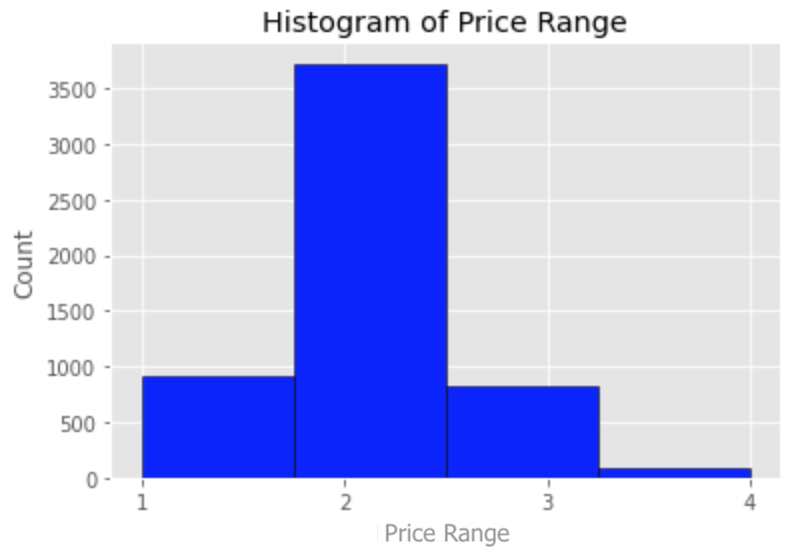
\includegraphics[width=350pt]{./images/4RestaurantsPriceRangeDistribution.png}
\caption{Restaurant’s Price Range Distribution}\label{fig:4RestaurantsPriceRangeDistribution}
\end{figure}\vspace{-24pt}

Figure~\ref{fig:4RestaurantsPriceRangeDistribution} shows the distribution of restaurants' price range. Price range level 2, 100 - 250 baht, is found in most restaurants, followed by level 1, lower than 100 baht, and level 3, 251 - 500 baht. The least price range found in our data is level 4, more than 500 baht. However, only 5,561 restaurants in our data specified their price range which is around 50\% of total restaurants.

\begin{figure}[H]\centering
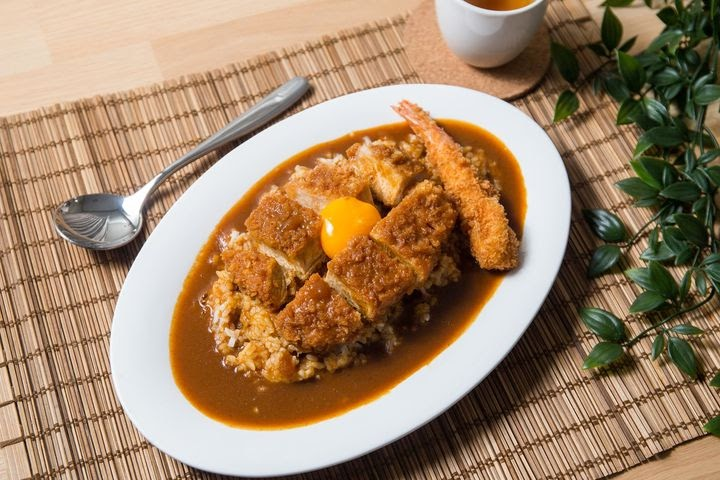
\includegraphics[width=350pt]{./images/4ExampleofRestaurantPicturefromFacebookPage.jpeg}
\captionsource{Example of Restaurant Picture from Facebook Page}{https://www.facebook.com/100170491339440}\label{fig:4ExampleofRestaurantPicturefromFacebookPage}
\end{figure}\vspace{-24pt}
\vspace{1em}

Figure~\ref{fig:4ExampleofRestaurantPicturefromFacebookPage} is an example of a restaurant picture in our data. The picture came from the restaurant's Facebook page photo cover image. The image is a crucial part of considering a restaurant from our feedback. However, only 3,513 restaurants in our data contain pictures which are around only 30\%. This is also one issue that we need to improve in order to make users’ restaurant consideration easier.

\begin{figure}[H]\centering
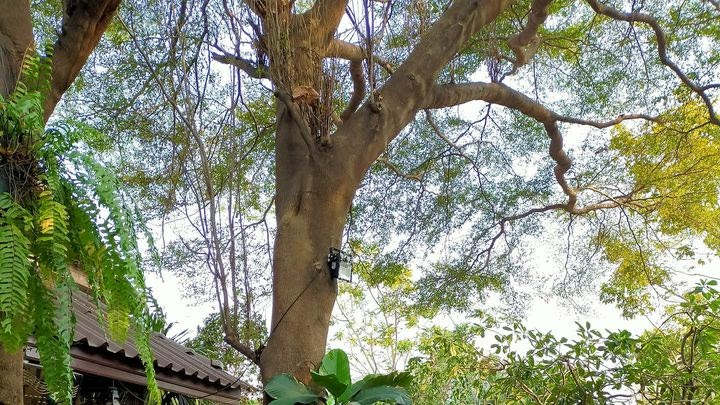
\includegraphics[width=350pt]{./images/4ExampleofUnrelatedRestaurantPicturefromFacebookPage.jpeg}
\captionsource{Example of Unrelated Restaurant Picture from Facebook Page}{https://www.facebook.com/100940911628308}\label{fig:4ExampleofUnrelatedRestaurantPicturefromFacebookPage}
\end{figure}\vspace{-24pt}
\vspace{1em}

However, from 3,513 restaurants in our data that contain images, their image is not quite related to the restaurant as the example in Figure~\ref{fig:4ExampleofUnrelatedRestaurantPicturefromFacebookPage}. This happens very commonly since all of the Facebook page data is user-generated data. We might overcome this problem by trying to get restaurant images from other sources.


\section{User Data Collection}

\subsection{Collection Process}

Our system needs to do data analysis and we need user behavior data for training our model. From the previous step, we already got restaurant data, but we did not have user interaction data. The user interaction data needs to include user information, restaurant information, and an interaction between user and restaurant which is a rating of each user to restaurants.

To collect this data, we implemented a data collection tool that lets users register and rate the appeared restaurant from the system.

\begin{figure}[H]\centering
\includegraphics[height=350pt]{./images/4RegistrationPageoftheDataCollectionTool.png}
\caption{Registration Page of the Data Collection Tool}\label{fig:4RegistrationPageoftheDataCollectionTool}
\end{figure}\vspace{-24pt}

Figure~\ref{fig:4RegistrationPageoftheDataCollectionTool} shows the registration page of the data collection tool. This is the first page that interviewees see. They need to input their new username, general profile information such as gender and birthdate and food preference which let users select from hate to love.

\newpage
\begin{figure}[H]\centering
\includegraphics[height=400pt]{./images/4RatingPageoftheDataCollectionTool.png}
\caption{Rating Page of the Data Collection Tool}\label{fig:4RatingPageoftheDataCollectionTool}
\end{figure}\vspace{-24pt}

After interviewees registered, they will see 20 restaurants one by one filtered by their food preferences on the registration page and nearby restaurants. They have to rate each restaurant from their opinion whether that restaurant is interesting or not. The user interface of the rating process is shown in Figure~\ref{fig:4RatingPageoftheDataCollectionTool}. After they finished rating 20 restaurants, they can choose to have more suggestions or logout from the system.

After the tool is developed, we planned to separate the interview into 3 methods which are face-to-face interview, virtual interview, and an online survey. We set a goal to have a minimum of 100 people.

\newpage
\begin{figure}[H]\centering
\includegraphics[width=300pt]{./images/4FacetofaceInterviewProcess.png}
\caption{Face-to-face Interview Process}\label{fig:4FacetofaceInterviewProcess}
\end{figure}\vspace{-24pt}

For the first method, face-to-face interview, we do it in 2 different locations which are in KMUTT and Siam Square One to have a different demographic. The second method which is virtual interviewing, we held an interview via online calling. For the last method, we sent a survey link to other people and also posted it on social media.

We have a total of 143 interviewees, 22 people from face-to-face interviews which are 10 people from KMUTT and 12 people from Siam Square One, 12 people from virtual interviews, and 109 people from online surveys. The users' feedback from face-to-face interviews and virtual interviews are also collected.

\subsection{Preprocessing Process}

After data has been collected, we clean out the data from users that do not live in Bangkok because we only have Bangkok restaurants. Those users might come from the online survey that we posted on social media.

\subsection{Results}


We collected data from 143 people which contains 5,102 interaction data. The data include user demographics, restaurant information, and their rating for each restaurant. The visualizations of the collected data are described in the following section.

\begin{figure}[H]\centering
\includegraphics[width=450pt]{./images/4DistributionofPeoplesLocation.png}
\caption{Distribution of People’s Location}\label{fig:4DistributionofPeoplesLocation}
\end{figure}\vspace{-24pt}

Figure~\ref{fig:4DistributionofPeoplesLocation} shows the distribution of people’s location while doing the survey. The top 2 most locations are Thung Khru district which mainly KMUTT students and Pathum Wan district which is the center of Bangkok.

\begin{figure}[H]\centering
\includegraphics[width=250pt]{./images/4TotalNumberofInteractedRestaurantsperPerson.png}
\caption{Total Number of Interacted Restaurants per Person}\label{fig:4TotalNumberofInteractedRestaurantsperPerson}
\end{figure}\vspace{-24pt}

Figure~\ref{fig:4TotalNumberofInteractedRestaurantsperPerson} shows the total number of interacted restaurants per person. Most people interact with 20 restaurants, which is the minimum number, but there are a lot of people who kindly do 60 interactions. The average number of interactions is 36 restaurants. In total, we got a total of 5,102 interactions from this survey.

\begin{figure}[H]\centering
\includegraphics[width=250pt]{./images/4VisualizationofPeoplesDemographic.png}
\caption{Visualization of People’s Demographic}\label{fig:4VisualizationofPeoplesDemographic}
\end{figure}\vspace{-24pt}

Figure~\ref{fig:4VisualizationofPeoplesDemographic} shows the summary of demographics in our data. The left visualization in Figure~\ref{fig:4VisualizationofPeoplesDemographic} shows the gender distribution which is almost half-and-half for males and females. The right visualization shows the age distribution. The highest age range in our data is the age of 20 to 25 years old. There are also a few people aged around 30 to 35 years old and more than 50 years old only a little.

\begin{figure}[H]\centering
\includegraphics[width=250pt]{./images/4AverageScoreofEachRestaurantCategoryfromPeople.png}
\caption{Average Score of Each Restaurant Category from People}\label{fig:4AverageScoreofEachRestaurantCategoryfromPeople}
\end{figure}\vspace{-24pt}

Figure~\ref{fig:4AverageScoreofEachRestaurantCategoryfromPeople} shows the average restaurant category score from all of our people. The score ranges from 0 to 100 which refers to hate and love respectively. The top three most favorite categories are Japanese restaurant, Thai restaurant, and shabu shabu restaurant respectively. The least favorite restaurant category is Chinese restaurants.

\begin{figure}[H]\centering
\includegraphics[width=200pt]{./images/4DistributionofUsersRatings.png}
\caption{Distribution of User’s Ratings}\label{fig:4DistributionofUsersRatings}
\end{figure}\vspace{-24pt}

Figure~\ref{fig:4DistributionofUsersRatings} shows the distribution of the user’s rating in our data from -2 which means the user is not interested in the restaurant to 2 which means the user is interested in that restaurant. The most rated score is 0 which is a neutral score.

This collected user behavior data will be used to be our data set for training the models in our system.


\subsection{Feedback}

Other than collecting the user behavior data, we also get the users’ feedback after they use our data collection tool in order to understand and get insight from each user in detail. We obtained feedback on our tool by asking face-to-face.

Firstly, we ask them about the pattern of their rating, what are the criteria to rate. From 22 people, most of them rated based on their preferences and the restaurant that they have visited. Furthermore, some of them rate a high score to an interesting restaurant that sometimes they have never visited before. Here is an example of feedback from a real user:

\begin{quote}{Pai, 20 years old}
“ My rating is based on the feeling of being like this restaurant is delicious while playing this application or clicking to the Facebook page and finding that it looks good to me. Moreover, some restaurants I have visited before, I will give it a high score.

Most of the 5 are my favorite restaurants and I have visited before. For an interesting restaurant but I have not visited yet, I will rate around 3 to 4.

For 1, in my point of view, the name of that restaurant not interest to me or some of the restaurant didn’t have a picture, so I don’t want to give it a high score ”
\end{quote}

Besides this, most of our users have similar scoring behaviors as this user which we can conclude and assume that if a user rating with 5 means that he/she has visited that restaurant already. By this assumption there will be implicit feedback for our recommendation system.

Then, we continue to ask that from our simple algorithm to recommend a restaurant, is there any interesting restaurant that matches your style. Surprisingly, 99\% of face-to-face users said that it can recommend a restaurant that matches their mind and if they are hungry, they will go to that restaurant. Below is the user that tends to go to the restaurant which comes from our suggestion.

\begin{quote}{Waranya, 23 years old}
“ I would like to go to the suggested restaurant, which is the first one from the system that recommended it to me. Moreover, for me, the picture of the restaurant plays a big role in restaurant consideration ”
\end{quote}

Lastly, we ask them if they have any suggestions for our system. We can conclude that they want to see more pictures of the restaurant with the recommended menu. So, we have to find another way to find a picture of the restaurant that has no picture. Also, for the restaurant’s menu problem, we currently cannot find a solution to this problem. Furthermore, the price preference in the registration part usually confuses them, so we already changed from only the Thai Baht ({\thaifont ฿}) interface to the Thai Baht with a price range for better understanding.

\subsection{Training Data Usage}

From our first plan in the first semester, we need to collect user behavior data for our model training process. We used this data to do an experiment on a collaborative filtering approach. However, we decided to change our recommendation system implementation to use the genetic algorithm in the second semester. This approach does not need any data to learn, so we did not use this training dataset for our final recommendation system.


\section{User Journey Finalization}

After we have done research, tested our user journey designed in the first semester, and received suggestions from our committees and our advisor, our user journey has been changed. Our final user journey of our application has been modified in 4 main aspects: login and registration, home screen, individual recommendation, and group recommendation.


\subsection{Login and Registration}

\begin{figure}[H]\centering
\includegraphics[width=350pt]{./images/4LoginandRegistrationUserJourneyChanges.png}
\caption{Login and Registration User Journey Changes}\label{fig:4LoginandRegistrationUserJourneyChanges}
\end{figure}\vspace{-24pt}

The main change in the login and registration process is our system requires food preference information in order to generate the suggestion. In the first semester, we plan to do login as a guest which users are not required to set their preference and they can skip the preference setting in the registration, so we need to eliminate those flow out. As a result of the final user journey, users who want to register for an account must set their food preference before using our system.

\subsection{Home Screen}

\begin{figure}[H]\centering
\includegraphics[width=350pt]{./images/4HomeScreenUserJourneyChanges.png}
\caption{Home Screen User Journey Changes}\label{fig:4HomeScreenUserJourneyChanges}
\end{figure}\vspace{-24pt}

In the previous semester, we assumed that users need to access the recommendation as fast as possible. We then designed it to have an individual recommendation as a home screen and users have to put a group pin code to enter a group recommendation. However, our advisor suggested that it will be confusing when people want to do a group recommendation and we all agreed that it is too hard to navigate to each functionality. As a result for the final user journey, we decided to add a home screen to our system which will help users use our application easier and eliminate the confusing navigation problem.

\subsection{Individual Recommendation}

\begin{figure}[H]\centering
\includegraphics[width=280pt]{./images/4IndividualRecommendationUserJourneyChanges.png}
\caption{Individual Recommendation User Journey Changes}\label{fig:4IndividualRecommendationUserJourneyChanges}
\end{figure}\vspace{-24pt}

In the first semester, the individual recommendation process is that users will see one suggested restaurant at a time and they have to select whether to go or not go to that shown restaurant. However, since we collected the feedback from users, we found that they wanted to see all of the suggested choices before selecting their final restaurant that they wanted to go to. As a result, we change the recommendation process to show all suggested restaurants at a time to users. Users then have to choose only one of the suggested choices as a final restaurant.

\subsection{Group Recommendation}

\begin{figure}[H]\centering
\includegraphics[width=350pt]{./images/4GroupRecommendationUserJourneyChanges.png}
\caption{Group Recommendation User Journey Changes}\label{fig:4GroupRecommendationUserJourneyChanges}
\end{figure}\vspace{-24pt}

In our first design of the group recommendation, each member will see the same set of suggested restaurants and they have to select whether to go or not one by one. The recommendation will be finished when every member agrees to go to the same restaurant. However, our committees suggested that the recommendation might require group discussion. Therefore, they might need to see all of their choices for their group instead of individually choosing the restaurant one by one. The designed process also makes the decision time much longer if the group is too large and no one agrees on the same restaurant. As a result, we decided to change the process. The new process lets users see the same fixed-sized set of restaurants and they will see all of the suggested restaurants instead of one by one. The system will ask everyone to rank the restaurants by their preferences. After every member finishes ranking restaurants, the system will finalize a final decision to the group.


\section{Web Application Result}

The web application result includes the results of server-side services as well as the results of the user interface or client-side service. The server-side services consist of 4 components: \textit{Data Service}, \textit{App Server}, \textit{Recommender}, and \textit{Database}, where the user interface result is from \textit{App Client}. The full source code is available at \url{https://github.com/restaurant-recommender}.

\subsection{Server-side Services Result}

\subsubsection{Data Service}

\begin{figure}[H]\centering
\includegraphics[width=200pt]{./images/4result_dataservice.png}
\caption{Restaurant Local Data from Facebook}\label{fig:4result_dataservice}
\end{figure}\vspace{-24pt}

This data service component is implemented as Python scripts. Figure~\ref{fig:4result_dataservice} shows the information about the local fetched data from Facebook. This data will be read and transformed into the right format before sending it to the \textit{App Server} to create a restaurant in the system.

\subsubsection{App Server}

\textit{App Server} is implemented with TypeScript with Express web framework and has been deployed on Google Cloud App Engine. This component needs to listen to other components’ requests. The API specification is described in Table~\ref{tbl:4AppServerAPISpecification} below.

\begin{table}[H]
\caption{App Server API Specification}\label{tbl:4AppServerAPISpecification}
\begin{tabularx}{\textwidth}{l|l|X} \hline\hline
Method & Path & Description \\ \hline\hline
\multicolumn{3}{l}{\textbf{Authentication}} \\ \hline\hline
POST & /api/auth & Request for authentication token for user login\\ \hline\hline
\multicolumn{3}{l}{\textbf{Users}}\\ \hline\hline
GET & /api/users/<id> & Get user profile from user object id \\ \hline
PUT & /api/users/<id> & Update user information \\ \hline
PUT & /api/users/<id>/profile\_weight & Update user preference weights \\ \hline
POST & /api/users & Create a new user \\ \hline
GET & /api/users/has/<username> & Check whether is username is already existed in the system\\ \hline\hline
\multicolumn{3}{l}{\textbf{Restaurants}}\\ \hline\hline
GET & /api/restaurants/nearby & Get nearby restaurant by specifying coordination \\ \hline
GET & /api/restaurants/search & Get restaurant by search query string \\ \hline
POST & /api/restaurants & Create a new restaurant \\ \hline
PUT & /api/restaurants/<id> & Update restaurant information \\ \hline\hline
\multicolumn{3}{l}{\textbf{Restaurant’s Categories}}\\ \hline\hline
GET & /api/categories/search & Get category by search query string \\ \hline
PUT & /api/categories/<id> & Update category information \\ \hline
POST & /api/categories & Create a new category \\ \hline\hline
\multicolumn{3}{l}{\textbf{Recommendations}}\\ \hline\hline
POST & /api/recommendations/init & Request for recommendation initialization this has to be called before getting the recommendation. \\ \hline
POST & /api/recommendations/request & Get recommendation \\ \hline\hline
\end{tabularx}
\end{table}

\subsubsection{Recommender}

\textit{Recommender} is implemented with Python with Flask web framework and has been deployed on Google Cloud App Engine. This component needs to listen to other \textit{App Server}’s requests. The API specification is described in Table~\ref{tbl:4RecommenderAPISpecification} below.

\begin{table}[H]
\caption{Recommender API Specification}\label{tbl:4RecommenderAPISpecification}
\begin{tabularx}{\textwidth}{l|l|X} \hline\hline
Method & Path & Description \\ \hline\hline
POST & /recommend/<type> & Request a set of suggested restaurants. “type” is needed to specify a different version of the recommendation model. \\ \hline\hline
\end{tabularx}
\end{table}

\subsubsection{Database}

\begin{figure}[H]\centering
\includegraphics[width=400pt]{./images/4mongodashboard.png}
\caption{Group Recommendation User Journey Changes}\label{fig:4mongodashboard}
\end{figure}\vspace{-24pt}

Our NoSQL database is deployed on MongoDB Atlas which is an official cloud deployment tool for MongoDB. Figure~\ref{fig:4mongodashboard} shows the monitoring dashboard of our database.


\subsection{User Interface Result}

Our user interface implementation has a lot of changes from our design since we do the testing from our design and committees’ suggestions. The main changes are recommendation flow and home screen. The recommendation flow is changed both for individual and group. In the individual flow, the application will show multiple restaurants instead of show it one-by-one. In the group flow, every member needs to rank the shown restaurant instead of keep finding the restaurant that they all agreed on. Lastly, in the first design, users will see an individual recommendation right away when they are logged in, so in the final implementation, we add a home screen for better navigation for users and easier to understand.

In the following sections, we will present our final user interface implementation including login, registration, home screen, individual recommendation, group recommendation, and favorite list.


\newpage
\subsubsection{Login}
\begin{figure}[H]\centering
\includegraphics[height=300pt]{./images/4ui_LoginPageUserInterface.png}
\caption{Login Page User Interface}\label{fig:4ui_LoginPageUserInterface}
\end{figure}\vspace{-24pt}

\begin{enumerate}
\item Username and password fields let users type their account’s username and password.
\item Login button lets users confirm their login information.
\item Register link button takes users to the registration page.
\end{enumerate}

When users open the application for the first time, they will see the login page. On this page, users can put their username and password in the above fields (1). After that, they can tap on the Login button (2) to continue. The system will validate the input information and let the user see the home screen. However, if they do not have any account yet, they can tap on the Register link button (3) to go to the registration page.

\newpage
\subsubsection{Registration}
\begin{figure}[H]\centering
\includegraphics[height=300pt]{./images/4ui_RegistrationUserInterface.png}
\caption{Registration User Interface}\label{fig:4ui_RegistrationUserInterface}
\end{figure}\vspace{-24pt}

\begin{enumerate}
\item New username and password input field.
\item Next button lets users continue the registration process.
\item Login link button takes users to the previous login page.
\item Food preference page lets users set their food preference.
\item Food preference ranking box let users reordering their food preference by dragging each food preference displayed in the list.
\item Done button lets users finish their registration process and access the home screen.
\end{enumerate}

The page is for users that do not have an account yet. They can choose their new username and password by inputting in the fields (1). They can tap on the Next button (2) to continue the process or go back to the login page by tapping the Login link button (3). After they tapped on the Next button (2), the food preference page (4) will be shown to the user. They need to rearrange the food preference items in the list to the love box (5) by dragging each item with a total of 5 selected items. After they select exactly 5 items, they can tap on the Done button (6) to finish the registration and they will be redirected to the home screen.

\newpage
\subsubsection{Home Screen}
\begin{figure}[H]\centering
\includegraphics[height=300pt]{./images/4ui_HomeScreenUserInterface.png}
\caption{Home Screen User Interface}\label{fig:4ui_HomeScreenUserInterface}
\end{figure}\vspace{-24pt}

\begin{enumerate}
\item Individual Eating button takes users to individual recommendation confirmation pages.
\item Group Eating section lets users create and join groups for a group recommendation.
\item Your Favorite button takes users to their favorite restaurant list page.
\item Edit Preference button takes users to the previous food preference page to edit their preference again.
\item About button takes users to the about section.
\item Logout Button let users sign out from the system.
\end{enumerate}

After users are logged in or complete the registration, they will see the home screen page shown in Figure~\ref{fig:4ui_HomeScreenUserInterface}. In this page, users can navigate to individual eating (1), group eating (2), favorite restaurant list (3), edit preference page (4) and about page (5). Users can log out by tapping on the Logout button (6).
\begin{figure}[H]\centering
\includegraphics[height=300pt]{./images/4ui_LanguageSwitchingUserInterface.png}
\caption{Language Switching User Interface}\label{fig:4ui_LanguageSwitchingUserInterface}
\end{figure}\vspace{-24pt}

\begin{enumerate}
\item Switch language button lets users change the display language for an entire application.
\end{enumerate}

Our application supports multiple display languages which include Thai and English. Users can switch the display language with the home screen from the top button labelled “{\thaifont ไทย}” or “EN”. Note that when switching the language, not only the home screen display language will be changed, but also an entire application.

\newpage
\subsubsection{Individual Recommendation}
\begin{figure}[H]\centering
\includegraphics[height=300pt]{./images/4ui_IndividualRecommendationConfirmationUserInterface.png}
\caption{Individual Recommendation Confirmation User Interface}\label{fig:4ui_IndividualRecommendationConfirmationUserInterface}
\end{figure}\vspace{-24pt}

\begin{enumerate}
\item Map lets users see the recommendation location or change the pin to desired location. It can be zoomed in and out and panned to any direction.
\item Search location button lets users search a location by keyword.
\item Target recommendation type selection includes restaurant, dessert shop and bar.
\item Prefer price selection includes cheaper than 100 baht, 100 - 250 baht, 250 - 500 baht, and more than 500 baht.
\item Next button lets users start an individual recommendation with the current setting.
\end{enumerate}

When users tap on the individual eating button in the home screen, users will see this individual confirmation page before starting the recommendation. In this confirmation page, users can change the recommendation location in the map (1) by panning to the target location or search location by keyword (2), change target recommendation type (3), and their preferred price (4). If users are satisfied with their setting, they can tap on the Start button (5) to start an individual recommendation.
\begin{figure}[H]\centering
\includegraphics[height=300pt]{./images/4ui_IndividualRecommendationUserInterface.png}
\caption{Individual Recommendation User Interface}\label{fig:4ui_IndividualRecommendationUserInterface}
\end{figure}\vspace{-24pt}

\begin{enumerate}
\item Recommended restaurant list.
\item Detail of each restaurant. When users tap on each restaurant, the restaurant item will be expanded to show more information.
\item Save to your favorite button lets users save each restaurant to their favorite list.
\end{enumerate}

When users start the individual recommendation, they will see 10 suggested restaurants shown in the list (1). They can choose to see an additional 10 restaurants at the end of the list. They can tap on each restaurant to see the details (2) and tap it again to collapse it. Moreover, they can add each restaurant to their favorite restaurant list by tapping the save button (3).
\begin{figure}[H]\centering
\includegraphics[height=300pt]{./images/4ui_IndividualRecommendationSelectionUserInterface.png}
\caption{Individual Recommendation Selection User Interface}\label{fig:4ui_IndividualRecommendationSelectionUserInterface}
\end{figure}\vspace{-24pt}

\begin{enumerate}
\item Users can choose their target restaurant by dragging them into the Love box.
\item Finish button lets users finish the recommendation. This button will be available only if users select exactly 1 restaurant.
\end{enumerate}

The goal of the individual recommendation page is to choose exactly one restaurant to be the target restaurant. The process can be done by dragging the restaurant that users want into the Love box. They can select more than 1 restaurant from the box above, but ultimately, they need to clear the selected list to have only 1 restaurant in order to finish the recommendation. Finally, if they want to finish the recommendation, they can tap on Finish button (2) to complete the current recommendation.
\begin{figure}[H]\centering
\includegraphics[height=300pt]{./images/4ui_IndividualRecommendationSuccessUserInterface.png}
\caption{Individual Recommendation Success User Interface}\label{fig:4ui_IndividualRecommendationSuccessUserInterface}
\end{figure}\vspace{-24pt}

\begin{enumerate}
\item Recommendation rating dialog lets users rate how satisfied they were with the recommendation.
\item Restaurant detail of the final restaurant.
\item Home button takes users back to the home screen.
\end{enumerate}

After users finish the recommendation, the system will show the recommendation success page. The recommendation rating dialog will be prompted to let users rate the recommendation and use this score for the model's further improvement. Users can see the details of the selected restaurant (2) and go back to the home screen by tapping the Home button (3).

\newpage
\subsubsection{Group Recommendation}
\begin{figure}[H]\centering
\includegraphics[height=250pt]{./images/4ui_GroupCreatingUserInterface.png}
\caption{Group Creating User Interface}\label{fig:4ui_GroupCreatingUserInterface}
\end{figure}\vspace{-24pt}

\begin{enumerate}
\item Create Group button lets users create an eating group that other people can join.
\item Pin Code used for group joining for other people.
\item Share button lets users use QR code or a link to invite other people.
\item Group customization lets users who are a head of the group change the group setting.
\item Members list shows current members who are in the group. The crown icon indicates that the person is a head of the group.
\item QR code for invite other people
\item Copy link button lets users quickly share an invitation through the link.
\end{enumerate}

When a group of people want to start a group recommendation, they need to firstly create a group. Creating a group can be done by tapping the Create Group button (1) on the home screen. After that, the person who creates a group will see a group confirmation page (the middle screen on Figure~\ref{fig:4ui_GroupCreatingUserInterface}). The page contains group pin code (2) that lets other people join the group, group customization setting (4) that lets a head of the group change the group setting, and member list (5) that shows all current members on the group. Moreover, users can tap on the Share button (3) to open a share sheet which contains a QR code (6) and the copy link button (7), so that other members can join the group easier. However, this group cannot be started yet, because there is only one member, so users need to wait for the other members.
\begin{figure}[H]\centering
\includegraphics[height=300pt]{./images/4ui_GroupJoiningUserInterface.png}
\caption{Group Joining User Interface}\label{fig:4ui_GroupJoiningUserInterface}
\end{figure}\vspace{-24pt}

\begin{enumerate}
\item Join Group button makes a join group dialog appear to users.
\item Pin code input field lets users put their group pin code that they want to join.
\item Join button lets users join the group with the input pin code.
\end{enumerate}

Next, if other users want to join the created group, they can tap on the Join Group button (1) and the join group dialog will be prompted. The dialog lets users input the group pin code obtained from the created group. Lastly, users can tap on the Join button to enter the group if the group pin code is valid.
\begin{figure}[H]\centering
\includegraphics[height=300pt]{./images/4ui_JoinedGroupUserInterface.png}
\caption{Joined Group User Interface}\label{fig:4ui_JoinedGroupUserInterface}
\end{figure}\vspace{-24pt}

\begin{enumerate}
\item Updated member list.
\item Start button
\end{enumerate}

After other people have joined the group, the member list will be updated (1). Each member can set their own preferred price (2), however, one the head of the group can change the group setting. When all members join and  are ready to start a group recommendation, the head can tap on the Start button to start the group recommendation.
\begin{figure}[H]\centering
\includegraphics[height=250pt]{./images/4ui_GroupRecommendationUserInterface.png}
\caption{Group Recommendation User Interface}\label{fig:4ui_GroupRecommendationUserInterface}
\end{figure}\vspace{-24pt}

\begin{enumerate}
\item Drag the item to the box above and rearrange them by users preference.
\item Finish button for users who finished rearranging already.
\item Waiting dialog.
\end{enumerate}

When the group recommendation is started, every member will see the same set of the suggested restaurants. The goal of this group recommendation page is that every member needs to rearrange the shown restaurants by dragging the restaurant up and down (1) according to their preference. After users rearrange all of the 6 restaurants, they can tap on the Finish button (2) to submit their information. However, since the system needs to collect every member’s information, if there is someone who has not finished their rearranging yet, the waiting dialog will be shown (3).
\begin{figure}[H]\centering
\includegraphics[height=300pt]{./images/4ui_GroupRecommendationSuccessUserInterface.png}
\caption{Group Recommendation Success User Interface}\label{fig:4ui_GroupRecommendationSuccessUserInterface}
\end{figure}\vspace{-24pt}

\begin{enumerate}
\item Summary button brings up the summary of the recommendation.
\item Home button takes users back to the home screen.
\end{enumerate}

When every member taps on the Finish button on the previous page, the group recommendation success screen will be shown. This page is very similar to individual recommendations, but it has the Summary button (1) that shows the summary of ranking for each restaurant. Lastly, users can go back to the home screen by tapping the Home button (2).

\newpage
\subsubsection{Favorite List}
\begin{figure}[H]\centering
\includegraphics[height=250pt]{./images/4ui_FavoriteRestaurantListUserInterface.png}
\caption{Favorite Restaurant List User Interface}\label{fig:4ui_FavoriteRestaurantListUserInterface}
\end{figure}\vspace{-24pt}

\begin{enumerate}
\item Your Favorite button takes users to their favorite restaurant list page.
\item Favorite restaurant list page.
\end{enumerate}

Users can view their previous saved restaurant by tapping on the Your Favorite button (1) in the home screen and the favorite restaurant list page (2) will be shown to users. Users can view the restaurant information by tapping on each restaurant.


\section{Model Experiment}

In this first semester, we tried to use model-based recommendation which is a collaborative filtering technique. However, this technique requires a large amount of user behavior data and it is very complex for implementing group recommendation. In order to overcome this problem, we decided to change from collaborative filtering technique to genetic algorithm technique which does not require any primitive user behaviour data and it can be implemented to support both individual and group recommendation with a simpler structure. In sections~\ref{sec:dataset} -~\ref{sec:cf}, we describe the data set and present the first experiment with collaborative filtering that we did in the first semester. After that, the results of the genetic algorithm approach, which is the final design of our proposed algorithm, is presented in section~\ref{sec:ga}.

\subsection{Data Set} \label{sec:dataset}

To conduct the experiment, we use the data from our data collection process both restaurant and user behavior data, which contains 11,175 restaurants with restaurants’ profiles and 143 users with 5,102 users’ ratings.

\subsubsection{Data Preparation}

We select some columns of user behavior data to be used in this experiment including 'user\_id', 'username', 'res\_id', 'res\_name', and 'rating' as the Figure~\ref{fig:4SelectedColumnsfromUserBehaviorData} below.

\begin{figure}[H]\centering
\includegraphics[width=200pt]{./images/4SelectedColumnsfromUserBehaviorData.png}
\caption{Selected Columns from User Behavior Data}\label{fig:4SelectedColumnsfromUserBehaviorData}
\end{figure}\vspace{-24pt}

For ‘user\_id’ refers to the identification of the user which is in the form of object ID with a unique identifier as Figure~\ref{fig:4SelectedColumnsfromUserBehaviorData}, ‘username’ is the name of the user which cannot be duplicated, ‘res\_id’ refers to the identification of each restaurant with a unique identifier in the form of object ID as same as user\_id, ‘res\_name’ refers to the name of the restaurants which we already clean the duplicated restaurant out of a database, and ‘rating’ refers to the user’s rating for each restaurant which starts from -2 to 2 [-2, -1, 0, 1, 2].

\begin{figure}[H]\centering
\includegraphics[width=200pt]{./images/4UserIDinObjectIDPattern.png}
\caption{User ID in Object ID Pattern}\label{fig:4UserIDinObjectIDPattern}
\end{figure}\vspace{-24pt}

Thus, for our convenience, we converted ‘user\_id’ from object ID to real number or integer pattern and converted ‘rating’ from -2 to 2 into 1 to 5 which is the standard pattern for better understanding. Then, we will get the dataset as Figure~\ref{fig:4SampleofSelectedUserBehaviorData} below.

\begin{figure}[H]\centering
\includegraphics[width=350pt]{./images/4SampleofSelectedUserBehaviorData.png}
\caption{Sample of Selected User Behavior Data}\label{fig:4SampleofSelectedUserBehaviorData}
\end{figure}\vspace{-24pt}

For the restaurants’ dataset, we select some related columns which are ‘id’, ‘name’, ‘cats’, ‘cats\_ids’, ‘price\_range’, ‘rating’, ‘likes’, ‘lat’, and ‘lon’ as in the Figure~\ref{fig:4SelectedColumnsfromRestaurantsData}  below.

\begin{figure}[H]\centering
\includegraphics[width=200pt]{./images/4SelectedColumnsfromRestaurantsData.png}
\caption{Selected Columns from Restaurants Data}\label{fig:4SelectedColumnsfromRestaurantsData}
\end{figure}\vspace{-24pt}

In ‘id’ column refers to the unique identification of each restaurant which in object ID format, ‘name’ is the restaurants’ name, ‘cats’ refer to the category of each restaurant e.g. Thai restaurant, Korean restaurant, Fast food restaurant, etc. which ‘cat\_ids’ is the unique object ID of each category, ‘price\_range’ refers to the price of each restaurant which is -1 and 1 to 4 [-1, 1, 2, 3, 4] by -1 means there is no price preferences in that restaurant’s profile, 1 means price is lower than 100 baht, 2 means 100 - 250 baht, 3 means 251 - 500 baht, and 4 means more than 500 baht, ‘rating’ is the average rating of each restaurant which come from the Facebook page, ‘lat’ and ‘lon’ columns are the latitude and longitude of each restaurant.

\begin{figure}[H]\centering
\includegraphics[width=350pt]{./images/4SampleofSelectedRestaurantData.png}
\caption{Sample of Selected Restaurant Data}\label{fig:4SampleofSelectedRestaurantData}
\end{figure}\vspace{-24pt}

Figure~\ref{fig:4SampleofSelectedRestaurantData} is the example data of the selected restaurant that we are going to use in this experiment.

\subsection{Collaborative Filtering Technique} \label{sec:cf}

After data preparation, we start to build a restaurant recommender for individuals by using user-based collaborative filtering which we referenced from  \cite{BuildauserbasedcollaborativefilteringrecommendationengineforAnime}. By the way, this approach is just only one of several recommendation techniques. In user-based collaborative filtering, we assumed that if users like similar items, users are similar to each other too by we start to discover the similarity of users and then recommend the item of other similar users liked.

Let us give an example similar to this technique, Alice likes to go to restaurants A, B, and C. Bob likes to go to restaurants A and B. Alice and Bob are similar due to the fact that they like restaurants A and B together and Alice has never seen restaurant C before. So, if we want to recommend a restaurant for Bob, we will recommend restaurant C.

\subsubsection{Discover the Similarity of Users}

We selected cosine similarities to be the methods to find the similarity. As we know that this method relies on vector representation which in this experiment will represent the users with a list of each restaurant ratings. We will represent it into a user-restaurant matrix with the rating values as Figure~\ref{fig:4SomePartoftheUserrestaurantMatrix} below.

\begin{figure}[H]\centering
\includegraphics[width=350pt]{./images/4SomePartoftheUserrestaurantMatrix.png}
\caption{Some Part of the User-restaurant Matrix}\label{fig:4SomePartoftheUserrestaurantMatrix}
\end{figure}\vspace{-24pt}

So, the more restaurants in the database, the more dimensionality per user by the value inside the matrix represents a rating from each user which 0 means that the user has not yet rated that restaurant. If the restaurants have been rated, it will show the number starting from 1 to 5 depending on the users’ rating.

\begin{figure}[H]\centering
\includegraphics[width=350pt]{./images/4FunctiontoFindaSimilarityBetweenUser.png}
\caption{Function to Find a Similarity Between User}\label{fig:4FunctiontoFindaSimilarityBetweenUser}
\end{figure}\vspace{-24pt}

Figure~\ref{fig:4FunctiontoFindaSimilarityBetweenUser} is a function to find a user similarity with cosine similarity by selecting only the top 3 users that have the most similarity to the target user. From this function, it will return the user ID of the top 3 users with a similarity score of each user with the target user as the example in Figure~\ref{fig:4ReturnValuefromsimilaruesrFunction} below.

\begin{figure}[H]\centering
\includegraphics[width=350pt]{./images/4ReturnValuefromsimilar_uesrFunction.png}
\caption{Return Value from similar\_user Function}\label{fig:4ReturnValuefromsimilaruesrFunction}
\end{figure}\vspace{-24pt}

From Figure~\ref{fig:4ReturnValuefromsimilaruesrFunction}, we try to find the similarity of users of user ID number 1. As a result, we get the top 3 user IDs with the highest similarity which is user ID numbers 3, 134, and 5 with the similarity scores of 0.8653, 0.8256, and 0.8086 respectively.

\subsubsection{Recommendation}

After we get the top 3 users that have the most similarity with the target user, next, we try to recommend the restaurant through these similar users.

\begin{figure}[H]\centering
\includegraphics[width=350pt]{./images/4RestaurantsRecommendationFunctionofUserbasedCollaborativeFilteringMethod.png}
\caption{Restaurants Recommendation Function of User-based Collaborative Filtering Method}\label{fig:4RestaurantsRecommendationFunctionofUserbasedCollaborativeFilteringMethod}
\end{figure}\vspace{-24pt}

We create a function to make a restaurant recommendation through a user-based collaborative filtering method as Figure~\ref{fig:4RestaurantsRecommendationFunctionofUserbasedCollaborativeFilteringMethod} by setting the function to recommend the top 10 recommended restaurants to users. We start to create a user-restaurant matrix of the top 3 users and then calculate the average ratings of each restaurant across 3 users. Moving on to our target user, we start to create a matrix similar to similar users and then generate a list of restaurants that the user has not seen yet which represent the value of 0.

Lastly, we get the average ratings from similar users to filter only restaurants that the target user has not seen but have ratings from the top 3 similar users. After that, we bring only the top 10 restaurants to recommend.

\begin{figure}[H]\centering
\includegraphics[width=350pt]{./images/4ExampleofTop10RecommendedRestaurantsforUser.png}
\caption{Example of Top 10 Recommended Restaurants for User}\label{fig:4ExampleofTop10RecommendedRestaurantsforUser}
\end{figure}\vspace{-24pt}

Figure~\ref{fig:4ExampleofTop10RecommendedRestaurantsforUser} is the final result from the recommend\_item function which recommends user ID number 1 by sorting the average ratings of the top 3 similar users from highest to lowest. As you can see from the figure, the category of each restaurant is in the same direction e.g. Thai restaurant category which occurs 3 times, or noodle house category which occurs 2 times.

\begin{figure}[H]\centering
\includegraphics[width=200pt]{./images/4AverageRatingsofTop10RecommendedRestaurants.png}
\caption{Average Ratings of Top 10 Recommended Restaurants}\label{fig:4AverageRatingsofTop10RecommendedRestaurants}
\end{figure}\vspace{-24pt}

Here are the average ratings of the top 10 restaurants for user ID number 1 as shown in Figure~\ref{fig:4AverageRatingsofTop10RecommendedRestaurants}. From our observation, we found that this user loves to eat noodles and usually gives the restaurant in this category a high score. So, our assumption that was mentioned in the theory of collaborative filtering, a group of people with similar tastes often tend to like similar items, is true.

However, the user-based collaborative filtering cannot serve our desires due to its limitation which is about the cold-start problem. New users in our platform cannot get a suitable recommendation for their preferences because this user has an empty list of preferences. Moreover, we discovered that this algorithm cannot recommend based on the location of the user, it just recommends based on the similarity of the user. For example, user A wants to get a recommendation from the Siam Paragon area, but her/his preference never rate the Siam Paragon area before and always rate the restaurant around KMUTT. As a result, the similarity of users to user A will be around KMUTT which cannot be recommended in the Siam Paragon area.

\subsection{Genetic Algorithm Technique} \label{sec:ga}

Since our project recommends restaurants for both individuals and groups, we need to examine how well the genetic algorithm works for both of them. The algorithm is implemented with Python by ourselves. The full code is provided in the appendix. In this section, we show the result of individual and group recommendation generation with rank aggregation in the group recommendation.

\subsubsection{Individual Recommendation Result}


\begin{figure}[H]\centering
\includegraphics[width=350pt]{./images/4SampleofIndividualsPreferences.png}
\caption{Sample of Individual’s Preferences}\label{fig:4SampleofIndividualsPreferences}
\end{figure}\vspace{-24pt}

\begin{figure}[H]\centering
\includegraphics[width=350pt]{./images/4ResultofIndividualRecommendationAlgorithm.png}
\caption{Result of Individual Recommendation Algorithm}\label{fig:4ResultofIndividualRecommendationAlgorithm}
\end{figure}\vspace{-24pt}

For individual recommendation results, we tested the algorithm with the sample of user’s preferences as Figure~\ref{fig:4SampleofIndividualsPreferences}. Besides, we selected Siam Paragon as a restaurant's recommendation location for this sample. The result after testing is not very effective as we can see from Figure~\ref{fig:4ResultofIndividualRecommendationAlgorithm} which this user gave Thai restaurants the first rank but the system recommends Thai restaurants only one restaurant. Nevertheless, the system recommends Japanese restaurants the most, including Sushi restaurants, which is the second rank of this user. To sum up, this restaurant recommendation algorithm is not very effective due to the restaurant data problems whether there is not enough type of restaurant around that location or incorrect restaurant tag.

\subsubsection{Group Recommendation Result}

\begin{figure}[H]\centering
\includegraphics[width=350pt]{./images/4SampleGroupofTwosPreferences.png}
\caption{Sample Group of Two’s Preferences}\label{fig:4SampleGroupofTwosPreferences}
\end{figure}\vspace{-24pt}

\begin{figure}[H]\centering
\includegraphics[width=350pt]{./images/4ResultofGroupRecommendationAlgorithm.png}
\caption{Result of Group Recommendation Algorithm}\label{fig:4ResultofGroupRecommendationAlgorithm}
\end{figure}\vspace{-24pt}

As a part of the group recommendation, developers tested the algorithm using a 2-member group with restaurant preferences as shown in  Figure~\ref{fig:4SampleGroupofTwosPreferences} and using Siam Paragon as a restaurant's recommendation location as well as individual recommendation. The system can recommend 6 restaurants according to the preferences of the members as shown in Figure~\ref{fig:4ResultofGroupRecommendationAlgorithm}. From the figure, we can see that all restaurants match with the users preferences including Korean, Thai and Japanese restaurants. Moreover, the fitness value of the generation dramatically increased to 75.

\subsubsection{Rank Aggregation Result}

\begin{figure}[H]\centering
\includegraphics[width=400pt]{./images/4SampleofSuggestedRestaurantsandRanksfromUsers.png}
\caption{Sample of Suggested Restaurants and Ranks from Users}\label{fig:4SampleofSuggestedRestaurantsandRanksfromUsers}
\end{figure}\vspace{-24pt}

\begin{figure}[H]\centering
\includegraphics[width=350pt]{./images/4FinalScorefromtheSample.png}
\caption{Final Score from the Sample}\label{fig:4FinalScorefromtheSample}
\end{figure}\vspace{-24pt}

After the genetic algorithm generates a set of suggested restaurants and lets each user rank the restaurants based on their preferences, rank aggregation finalizes that information to show the most suitable final restaurant for that group by computing the score for each restaurant. Figure~\ref{fig:4SampleofSuggestedRestaurantsandRanksfromUsers} shows the sample of generated restaurants that has shown to users and how each user ranks their restaurant. After that the rank aggregation algorithm calculates the score for each restaurant as stated in Figure~\ref{fig:4FinalScorefromtheSample}. As a result, the final restaurant for this input is a restaurant named Hua Pla Chongnonsea with a highest score of 3.4. This result shows that our finalization process considers not only users’ ranking but also restaurant’s type and cost.


\section{Evaluation Result}

\subsection{User Evaluation}

We divided the user evaluation into two rounds. In the first user evaluation, we rather focus on the user interface in order to modify it before the final evaluation while in the final user evaluation we focus on both the user interface and the recommendation algorithm.

\subsubsection{First User Interface Evaluation}

Developers have tested a restaurant recommendation system for both individuals and groups with some groups of users and it has been found that most of the users say the system is easy to use and can recommend a restaurant that meets their interests well. Thus, it is quite satisfying to users but there are still some parts that need to be resolved e.g. revised user interface for more ease to use, etc.

\textbf{Individual Recommendation Feedback}\par

For the individual part, we let users get the restaurant recommendation from their own location and we found that there are very few restaurants to recommend to that area, if not in downtown such as Siam Square. However, after we get feedback from users, most users still can receive restaurant recommendations that match with their preferences but it is not as much as they expected. So, our quick solution is to extend the distance between the restaurant and the user more from 1 kilometer to 3 kilometers.

\begin{figure}[H]\centering
\includegraphics[width=350pt]{./images/4usereva1.jpg}
\caption{Revised an Individual Recommendation System Interface}
\label{fig:4usereva_1}
\end{figure}\vspace{-24pt}

The next issue is about the individual recommendation interface as shown in  Figure~\ref{fig:4usereva_1} on the left. Most users said that they do not want to choose and stop immediately because they would rather have the previous restaurant but cannot go back anymore. In short, they want to compare the recommended restaurants. So, we revised the user interface of this page as shown in Figure~\ref{fig:4usereva_1} on the right. The new one can let the user compare each restaurant easily by recommending 10 restaurants per set.

Other feedback of the user interface is about the “Craving for...” selection bar from the settings page. Some users said that this interface looks quite confusing to them which leads to misunderstanding such as this bar can select all categories, not just one. Thus, we decided to change from this interface to the dropdown menu instead for both individual and group recommendation.

Last topic to concern is about the distance between users and recommended restaurants. At the moment, the system represents the distance by calculating the displacement but most users felt that it was too close than in reality. Our solution is to change the calculation method by calculating from the path of the car travelling e.g. Google Maps.

In summary, we need to change the user interface of the recommendation and preferences page for ease of use and change the distance calculation method to the path of car travelling instead.

\textbf{Group Recommendation Feedback}\par

For group recommendation feedback, most users said that the recommended restaurants can match with their preferences and interests as well as individual recommendation. For user interface feedback, there is one part of the recommendation process that needs to be changed which is the user’s waiting action. We found that a lot of users did not notice that they needed to wait for all members in the group to finish their ranking. They seem confused about what to do next. So, we need to change by giving them more interaction or creating a pop-up to notify them more clearly.

\subsubsection{Final User Evaluation}

After the first user evaluation, we revised some user interface both individual and group recommendation interfaces for more understanding and ease to use. This time, we tested a restaurant recommendation system on 41 users, using Google Forms to gather all feedback. This survey collected the user satisfaction with our recommendation, as well as the chance of  returning to use our recommender again.

We separated our Google Forms into 4 sections:basic information, individual recommendation satisfaction, group recommendation satisfaction, and overall satisfaction with the application.  In all satisfaction sections, we collect scores ranging from 1 to 5, with 5 indicating the most satisfied.

\textbf{Individual Recommendation Feedback}\par

More than half of the 41 people polled said that the recommended restaurants matched their preferences for both food and price, with 88\% and 76\%, respectively. Moreover, it has been found that around 63\% of the respondents can now decide which restaurant to eat more easily than before.

The detail of the recommended restaurant in the individual recommendation section is faultless. However, most of the respondents said that they would prefer more topics such as reviews of that restaurant. Overall feedback in the individual recommendation section is easy to use and can solve user’s pain more or less.

\textbf{Group Recommendation Feedback}\par

Due to the COVID-19 situation in Thailand, a lot of people are unable to go out and eat in groups. According to  further inquiries, most of the respondents are students who live alone in the dormitory. As a result, the number of respondents who can evaluate the group recommendation is lower than the number of respondents who can evaluate the individual recommendation. The group recommendation feedback has 14 respondents among 41.

From the evaluation, around 82\% of the respondents indicated that the system can recommend the restaurant that matches their food and price preferences. The majority of users are able to decide which restaurant to eat at with their own group. Moreover, the system can recommend a restaurant to a group of users at a glance.


\textbf{Conclusion}\par

In summary, 90.3\% of users said that this application is easy to use and not complicated due to the tutorial before use, which makes a lot of users easy to follow. In terms of the application interface, 87.9\% thought it is beautiful and convenient to use. The rest of the respondents thought it is quite good to use, and there was no negative feedback on this topic. Moreover, approximately 95\% said that this application can recommend the restaurant to both individuals and groups quickly. They do not have to wait too long. However, many people want more pictures and information about each restaurant, as well as a shorter process before reaching the recommendation page, or, in other words, to reduce human effort.

The average score for overall satisfaction is 4.2 out of 5. We can conclude that the restaurant recommendation system for individuals and groups was well-liked by the majority of users. Furthermore, approximately 87\% of users stated that they will return to use this application for their next meals.

\subsection{Application Performance Evaluation}

\begin{figure}[H]\centering
\includegraphics[width=350pt]{./images/4ApplicationPerformanceEvaluationRequest.png}
\caption{Application Performance Evaluation Request}\label{fig:4ApplicationPerformanceEvaluationRequest}
\end{figure}\vspace{-24pt}

For the application performance evaluation, we do the load test and monitor the latency of our main components: \textit{App Client}, \textit{App Server}, and \textit{Recommender}. The load test is performed with 100 concurrent requests which simulate the scenario that 100 users are using the application at the exact same time.

Figure~\ref{fig:4ApplicationPerformanceEvaluationRequest} shows a request for application performance evaluation. All 3 services can handle 100 concurrent requests without errors and have an average response time of 4,747.69 milliseconds. The longest response time is taken by \textit{Recommender}, which is 11,243 milliseconds. Note that this is a scenario in which 100 users request a recommendation at the same time. If the number of concurrent users is reduced, the response time will be significantly decreased. \textit{Recommender} also has the largest sent data size, which is 873.33 KB per second, because it needs a set of available nearby restaurants from the server. On the other hand, \textit{App Client} has the largest received data size since servers send entire reference pages, related scripts, and assets to users.

All of our evaluation is tested with the production server deployment and database. However, since we use Google Cloud Platform for our deployment, it supports auto scaling and manages all of the network traffic for us. As a result, it can accomodate more concurrent users and have improved performance. Although the auto scaling setup is very easy, the deployment cost would be charged considerably higher. Another reason we cannot test with multiple instances is that Google Cloud Platform only allows us to run 1 instance per service, and our request to increase the quota was denied due to low utilization.

Although 100 concurrent requests is insufficient to conclude the efficiency of the services, it is adequate for the current development phase. We can use the deployed services to conduct open beta testing with no issues. Once we gain a larger number of usage from users, we can request more number of instance quotas from Google Cloud so that our services can serve a higher number of concurrent requests.

\subsection{Recommendation Evaluation}


\begin{figure}[H]\centering
\includegraphics[width=350pt]{./images/4LineGraphbetweenGenerationandFitnessValueofGeneticAlgorithm.png}
\caption{Line Graph between Generation and Fitness Value of Genetic Algorithm}\label{fig:4LineGraphbetweenGenerationandFitnessValueofGeneticAlgorithm}
\end{figure}\vspace{-24pt}

We evaluated our recommendation algorithm by observing and analyzing the performance from the line graph as shown in Figure~\ref{fig:4LineGraphbetweenGenerationandFitnessValueofGeneticAlgorithm}. Each line in the figure represents each fitness generation by running ten times to compare each run time and check the existence of the local maximum problem. The results present that all run times can increase their fitness through generation continuously even though each run time does not start at the same value. Besides that not once was stuck at the local maximum as we can see from this graph that all of them terminate themselves after reaching fitness value equal to 66. So, we will continue to stick with these parameters as represented in Figure~\ref{fig:4ParametersofGeneticAlgorithminthisRecommender}.

\begin{figure}[H]\centering
\includegraphics[width=200pt]{./images/4ParametersofGeneticAlgorithminthisRecommender.png}
\caption{Parameters of Genetic Algorithm in this Recommender}\label{fig:4ParametersofGeneticAlgorithminthisRecommender}
\end{figure}\vspace{-24pt}

We set up for one generation to have 100 chromosomes by selecting the top 30 chromosomes to be paired up 50 pairs for reproduction. Moreover, the rate of crossover and mutation are 0.7 and 0.5 respectively. We keep this number to balance the exploration and exploitation which are able to make the performance better.

However, the results from this graph show us that we can reduce the number of termination conditions which is 15 to lower.

\begin{figure}[H]\centering
\includegraphics[width=350pt]{./images/4GeneticAlgorithmExecutionTimewith6Genes.png}
\caption{Genetic Algorithm Execution Time with 6 Genes}\label{fig:4GeneticAlgorithmExecutionTimewith6Genes}
\end{figure}\vspace{-24pt}

\begin{figure}[H]\centering
\includegraphics[width=350pt]{./images/4GeneticAlgorithmExecutionTimewith10Genes.png}
\caption{Genetic Algorithm Execution Time with 10 Genes}\label{fig:4GeneticAlgorithmExecutionTimewith10Genes}
\end{figure}\vspace{-24pt}

We measure the execution time of our genetic algorithm implementation. Figure~\ref{fig:4GeneticAlgorithmExecutionTimewith6Genes} shows the execution time with the total number of 6 genes in each chromosome which is used in group recommendation. The average execution time is 81 milliseconds. Figure~\ref{fig:4GeneticAlgorithmExecutionTimewith10Genes} shows the execution time with the total number of 10 genes in each chromosome which is used in individual recommendation. The average execution time is 165 milliseconds. We can conclude that the algorithm can deliver a fast suggestion generation with less than 1 second of both individual and group recommendations. Moreover, if we reduce the number of termination conditions, we can save even more execution time.



%%%%%%%%%%%%%%%%%%%%%%%%%%%%%%%%%%%%%%%%%%%%%%%%%%%%%%%%%%%%%%%%%%%%%%%%%%%
%%%%%%%%%%%%%%%%%%%%%%%%%%%%%%%%%%%%%%%%%%%%%%%%%%%%%%%%%%%%%%%%%%%%%%%%%%%
%%%%%%%%%%%%%%%%%%%%%%%%%%%%%%%%%%%%%%%%%%%%%%%%%%%%%%%%%%%%%%%%%%%%%%%%%%%
%%%%%%%%%%%%%%%%%%%%%%%%%%%%%%%%%%%%%%%%%%%%%%%%%%%%%%%%%%%%%%%%%%%%%%%%%%%
%%%%%%%%%%%%%%%%%%%%%%%%%%%%%%%%%%%%%%%%%%%%%%%%%%%%%%%%%%%%%%%%%%%%%%%%%%%


\chapter{Conclusions}

\section{Problems and Solutions}

\subsection{User and Restaurant Data}

Our project heavily relies on dataset both restaurant and user behavior data. However, the data we need for this project is not publicly available. Most of the dataset we found is from other countries, but we aim to develop this system for Thai people. The information about restaurant categories and user behavior of Thai people and other countries is different from each other.

To solve this problem, we need to collect the data by ourselves which takes much longer than we expected. We try to find the public data that serves our system requirement. The restaurant data can be obtained by using Thai Chana and Facebook Graph API. The user behavior is collected by face-to-face and online interviews and online surveys.

Even though we can find public restaurant data, the data is not large enough to cover all of the restaurants in Bangkok. The restaurant data outside the center of Bangkok is still insufficient. From our tested results at KMUTT location, there are only 15 restaurants in a range of 1 kilometer. To solve this problem, we expanded the nearby range to be 3 kilometers which can find many more restaurants. However, in order to solve the insufficient data problem, we might need to find other data sources that can give us a higher number of restaurants.

\subsection{Restaurant Images from Facebook Page}
From our survey, we found that restaurant images are a major factor in restaurant consideration. People tend to choose restaurants from their photos which can show how tasty the food and restaurant environment are. However, only 30\% of restaurants in our database have images. Moreover, 30\% of restaurants contain unrelated images. Thus, only a few restaurants in our database have meaningful images that represent the food and their restaurant.

We cannot find the best approach to solve this problem yet. We try to add a default icon for the restaurants that do not have an image. However, adding a default icon does not help in the restaurant consideration process. Another approach is to use additional external services such as Google Place API to obtain images.

\subsection{Restaurant Duplication}
Since the restaurant data collected from Facebook page data, it does not guarantee that one restaurant can have only one Facebook page because it is user generated data. Because of that, our database contains duplicate restaurant data which is the problem. Users should not see the duplicate data in their suggestion.

To solve this issue, we create a duplication checking process to check the distance between 2 restaurants and the name similarity. The process will keep only more detailed restaurants in the database. This process can eliminate up to 2,000 restaurants which can clear almost all of the duplication. However, due to a human error in user generated data, some of the duplicated restaurants have incorrect location data which our checking process cannot detect because it is still out of checking distance range. So, there is some restaurant duplication in our database but it is very few which is acceptable.

\subsection{Restaurant Category Information}
The most important information needed in our system is restaurant categories such as Thai, Japanese and Korean restaurants. However, since we use Facebook page data which is user generated data to be our restaurant data, it has a main problem which is incorrect information. From our further investigation, we found that many restaurants in our database have incorrect restaurant category data. There is some restaurant that does not have a main category tag, for example, it has a sushi tag but it does not have a Japanese restaurant tag.

We solved a missing main tag problem by inserting the main tag for the related tags. For example, if the restaurant has a sushi tag, the system will insert Japanese tag automatically. However, with this solution, the system inserts the main tag for only 400 restaurants which is too less from our expectation. Thus, the restaurant category information is still an issue and the misinformation cannot be solved for all restaurants in our database.

\subsection{Restaurant Distance Information}

Currently, we calculate distance between users and restaurants using displacement from 2 coordinates. The problem with this calculation is that the calculated distance does not equal the actual route distance because the calculation does not consider the actual possible route on the map. Users frequently face the situation in which the shown distance is very short, but when they choose to see the actual route to the restaurant, it is much longer.

To solve this problem, we can use additional route generating API, such as Google Map API. However, since we want to keep a simple structure for a current development phase and keep our billing costs as low as possible, this solution is planned to be our future work.

\section{Future Works}

We can divide our future works into 3 parts which are dataset, web application and recommendation improvement. In the dataset improvement, we could improve the restaurant image problem by using other external services or try to find alternative data sources that provide us more accurate information. In web application improvement, we plan to add a group chat feature to improve the discussion process in group recommendation. Lastly, in the recommendation improvement, we can try to tune the parameters and do more experiments of our genetic algorithm, so the performance and users’ satisfaction will be increased.

\begin{figure}[H]\centering
\includegraphics[width=400pt]{./images/5LINEMiniAppIntegration.png}
\caption{LINE Mini App Integration}\label{fig:5LINEMiniAppIntegration}
\end{figure}\vspace{-24pt}

Moreover, in the web application improvement, we could integrate our existing application with LINE Mini App. Figure~\ref{fig:5LINEMiniAppIntegration} shows the 3 main benefits from this integration. The first is that users can easily add our application to their LINE home screen without any installation. Next, users can invite friends via individual and group LINE chat. Lastly, users can easily see and join a group within LINE chat.

\section{Conclusion}

Restaurant recommendation system for individuals and groups is a web application with a recommendation system which supports Thai restaurants located in Bangkok. The web application makes users access and use the recommendation system at ease. It provides a friendly user interface to people. The recommendation system is implemented with the genetic algorithm which supports both individual and group recommendation with a simple structure. It can generate a decent suggestion and consume only little execution time. Our system can reduce time taken for restaurant decision making. From our feedback gathering, people are mostly satisfied with our recommendation. For further improvement, we could improve our restaurant dataset and tune our genetic algorithm to generate even more pleasant suggestions.


%%%%%%%%%%%%%%%%%%%%%%%%%%%%%%%%%%%%%%%%%%%%%%%%%%%%%%%%%%%%%%%
%%%%%%%%%%%%%%%%%%%% Bibliography %%%%%%%%%%%%%%%%%%%%%%%%%%%%%
%%%%%%%%%%%%%%%%%%%%%%%%%%%%%%%%%%%%%%%%%%%%%%%%%%%%%%%%%%%%%%%

%%%% Comment this in your report to show only references you have
%%%% cited. Otherwise, all the references below will be shown.
%\nocite{*}
%% Use the kmutt.bst for bibtex bibliography style 
%% You must have cpe.bib and string.bib in your current directory.
%% You may go to file .bbl to manually edit the bib items.
\bibliographystyle{kmutt}
\bibliography{string,cpe}

%%%%%%%%%%%%%%%%%%%%%%%%%%%%%%%%%%%%%%%%%%%%%%%%%%%%%%%%%%%%%%%
%%%%%%%%%%%%%%%%%%%%%%%% Appendix %%%%%%%%%%%%%%%%%%%%%%%%%%%%%
%%%%%%%%%%%%%%%%%%%%%%%%%%%%%%%%%%%%%%%%%%%%%%%%%%%%%%%%%%%%%%%
\appendix{Restaurant Considerations Survey}
\noindent{\large\bf Restaurant Considerations Survey} \\

We conduct the restaurant consideration survey in order to understand the user behavior and validate the problem to make sure that it is existing, not just our opinion.

\begin{figure}[H]\centering
\includegraphics[width=350pt]{./images/A1RestaurantConsiderationSurveyinGoogleform.png}
\caption{Restaurant Consideration Survey in Google form}\label{fig:A1RestaurantConsiderationSurveyinGoogleform}
\end{figure}\vspace{-24pt}

In this survey, we separated into 4 parts which are basic information, individuals eating consideration, groups eating consideration, and experience of using recommendation applications.

We surveyed by sharing the Google form through social media platforms e.g. Facebook, Instagram, etc. By having 148 respondents who have done the problem validation survey. Here are the results of this survey.

\textbf{Part 1: Basic Information}

\begin{figure}[H]\centering
\includegraphics[width=350pt]{./images/A1GenderofRespondents.png}
\caption{Gender of Respondents}\label{fig:A1GenderofRespondents}
\end{figure}\vspace{-24pt}

From the survey, 66.2\% were female, 32.4\% were male, and unspecified gender 1.4\% which concluded into 148 respondents.

\begin{figure}[H]\centering
\includegraphics[width=350pt]{./images/A1DistributionofRespondentsAge.png}
\caption{Distribution of Respondents’ Age}\label{fig:A1DistributionofRespondentsAge}
\end{figure}\vspace{-24pt}

As Figure~\ref{fig:A1DistributionofRespondentsAge} showed us the distribution of respondents’ age, we found that the most age range is around 19 - 23 years old which the interviewees mostly have the age range of 21 years old with 24.3\%.


\begin{figure}[H]\centering
\includegraphics[width=350pt]{./images/A1OccupationofRespondents.png}
\caption{Occupation of Respondents}\label{fig:A1OccupationofRespondents}
\end{figure}\vspace{-24pt}

The most occupation of our respondents are students with 52.7\% and followed by office workers 26.4\%. Moreover, this pie chart is related to the distribution of respondents’ age, with the most age range being around 19 - 23 years old which is the range of students in Thailand.

\begin{figure}[H]\centering
\includegraphics[width=350pt]{./images/A1EstimatedDailyCostofEating.png}
\caption{Estimated Daily Cost of Eating}\label{fig:A1EstimatedDailyCostofEating}
\end{figure}\vspace{-24pt}

Figure~\ref{fig:A1EstimatedDailyCostofEating}, The most eating cost per day is 200 baht with 32.4\% or 48 out of 148 respondents. As you can see from the figure, a few respondents have a lot of budget for eating per day which the maximum budget is 4,000 baht.

\begin{figure}[H]\centering
\includegraphics[width=350pt]{./images/A1TheApplicationorPlatformthatRespondentUsuallyUsetoFindtheRestaurants.png}
\caption{The Application or Platform that Respondent Usually Use to Find the Restaurants}\label{fig:A1TheApplicationorPlatformthatRespondentUsuallyUsetoFindtheRestaurants}
\end{figure}\vspace{-24pt}

In summary, they usually find the restaurant from the delivery platform e.g. Grab, Get, Lineman, etc. From search engines like Google and applications that gather restaurants in one place like Wongnai and so on.

\newpage
\textbf{Part 2: Individuals Eating Consideration}

\begin{figure}[H]\centering
\includegraphics[width=350pt]{./images/A1Top3ConditionstoFindtheRestaurantwhenEatingAlone.png}
\caption{Top 3 Conditions to Find the Restaurant when Eating Alone}\label{fig:A1Top3ConditionstoFindtheRestaurantwhenEatingAlone}
\end{figure}\vspace{-24pt}

As you can see from Figure~\ref{fig:A1Top3ConditionstoFindtheRestaurantwhenEatingAlone}, the condition that concerns them the most when eating alone is the price followed by the quality of food then available for delivery. Moreover, they are still concerned about the distance between them and the restaurant too.

\begin{figure}[H]\centering
\includegraphics[width=350pt]{./images/A1AverageTimetoSelecttheRestaurantAlone.png}
\caption{Average Time to Select the Restaurant Alone}\label{fig:A1AverageTimetoSelecttheRestaurantAlone}
\end{figure}\vspace{-24pt}

From Figure~\ref{fig:A1AverageTimetoSelecttheRestaurantAlone}, the most range of time that respondents spend to select the restaurant in an individual is 5 - 10 minutes with 40.5\% followed by 10 - 30 minutes which 35.1\% Furthermore, we notice that with 11.5\% they said that depending on the period.

\begin{figure}[H]\centering
\includegraphics[width=350pt]{./images/A1NumberofRespondentsThinkingthatRestaurantSelectionisTheirPain.png}
\caption{Number of Respondents Thinking that Restaurant Selection is Their Pain}\label{fig:A1NumberofRespondentsThinkingthatRestaurantSelectionisTheirPain}
\end{figure}\vspace{-24pt}

We found that around 62.8\% of respondents have a problem with restaurant selection which can prove our assumption that making the decision to go to the restaurant for each meal is still a problem nowadays.

\begin{figure}[H]\centering
\includegraphics[width=350pt]{./images/A1WhichMealHasProblemtheMost.png}
\caption{Which Meal Has Problem the Most}\label{fig:A1WhichMealHasProblemtheMost}
\end{figure}\vspace{-24pt}

The meal that everyone has the most problem with is dinner time. In our opinion, we think that it is the first meal that everybody reunited again after work or study. So many people, many conditions, which leads to complex decision making.

\begin{figure}[H]\centering
\includegraphics[width=350pt]{./images/A1ProblemBetweenDine-inandDelivery.png}
\caption{Problem Between Dine-in and Delivery}\label{fig:A1ProblemBetweenDine-inandDelivery}
\end{figure}\vspace{-24pt}

In Figure~\ref{fig:A1RestaurantConsiderationSurveyinGoogleform}1, you can see that dine-in and delivery are almost half-and-half. For dine-in problems, they said that it is hard to find the restaurant and decisions cannot be made quickly but for delivery, they know which restaurant to eat due to the foods’ picture of each restaurant and dine-in needs to consider more conditions than delivery. For delivery problems, they said that it is hard to decide what to eat because there is an overwhelming amount of restaurants to choose from and the main condition needed to consider is the distance from the restaurant.

\newpage
\textbf{Part 3: Groups Eating Consideration}

\begin{figure}[H]\centering
\includegraphics[width=350pt]{./images/A1AverageTimetoSelecttheRestaurantinGroup.png}
\caption{Average Time to Select the Restaurant in Group}\label{fig:A1AverageTimetoSelecttheRestaurantinGroup}
\end{figure}\vspace{-24pt}

From Figure~\ref{fig:A1RestaurantConsiderationSurveyinGoogleform}2, the most range of time that respondents spend to select the restaurant in a group is 5 - 10 minutes with 37.5\% followed by 10 - 30 minutes which 32.4\% Furthermore, we notice that 18.2\% of respondents spend time more than 30 minutes which 3 times Three times the number of people compare to individual.

\begin{figure}[H]\centering
\includegraphics[width=350pt]{./images/A1NumberofRespondentsThinkingthatRestaurantSelectioninGroupisTheirPain.png}
\caption{Number of Respondents Thinking that Restaurant Selection in Group is Their Pain}\label{fig:A1NumberofRespondentsThinkingthatRestaurantSelectioninGroupisTheirPain}
\end{figure}\vspace{-24pt}

We found that around 65.5\% of respondents have a problem with restaurant selection in groups which compared to individual problems, has increased up to 2.7\%. Thus, we can conclude that people faced more pain with group eating than individuals.

\begin{figure}[H]\centering
\includegraphics[width=350pt]{./images/A1TheFrequencyofGroupEatingProblems.png}
\caption{The Frequency of Group Eating Problems}\label{fig:A1TheFrequencyofGroupEatingProblems}
\end{figure}\vspace{-24pt}

From this figure, we found that respondents tend to have restaurant selection in group problems often.

\begin{figure}[H]\centering
\includegraphics[width=350pt]{./images/A1TheMostTypeofGroupthatUsuallyOccurGroupEatingProblem.png}
\caption{The Most Type of Group that Usually Occur Group Eating Problem}\label{fig:A1TheMostTypeofGroupthatUsuallyOccurGroupEatingProblem}
\end{figure}\vspace{-24pt}

Next, we want to know which group usually faces the pain of this problem. Figure~\ref{fig:A1RestaurantConsiderationSurveyinGoogleform}5 reveals that a group of friends usually faced the pain with 75.3\% and followed by family then, boyfriend/girlfriend.

\begin{figure}[H]\centering
\includegraphics[width=350pt]{./images/A1Top3ConditionstoFindtheRestaurantwhenEatingwithGroupofFriends.png}
\caption{Top 3 Conditions to Find the Restaurant when Eating with Group of Friends}\label{fig:A1Top3ConditionstoFindtheRestaurantwhenEatingwithGroupofFriends}
\end{figure}\vspace{-24pt}

The top 3 conditions are price, promotion, quality of the food which include the distance of the restaurant to be the condition to consider.

\begin{figure}[H]\centering
\includegraphics[width=350pt]{./images/A1Top3ConditionstoFindtheRestaurantwhenEatingwithFamily.png}
\caption{Top 3 Conditions to Find the Restaurant when Eating with Family}\label{fig:A1Top3ConditionstoFindtheRestaurantwhenEatingwithFamily}
\end{figure}\vspace{-24pt}

The top 3 conditions are quality of food, distance, and price which include the environment of the restaurant to be the condition to consider due to from 3 groups, only this group concerns the environment of the restaurants compared to the other.

\begin{figure}[H]\centering
\includegraphics[width=350pt]{./images/A1Top3ConditionstoFindtheRestaurantwhenEatingwithGirlfriend.png}
\caption{Top 3 Conditions to Find the Restaurant when Eating with Girlfriend/boyfriend}\label{fig:A1Top3ConditionstoFindtheRestaurantwhenEatingwithGirlfriend}
\end{figure}\vspace{-24pt}

The top 3 conditions are promotion, price, and quality which include the quality of services to be the condition to consider due to from 3 groups, only this group concerns the services compared to the other groups which are family and friends. As you can see, the conditions when eating are significantly different from each other.

\begin{figure}[H]\centering
\includegraphics[width=350pt]{./images/A1ReasonofProblemthatFrequentlyOccurswhenEatinginGroup.png}
\caption{Reason of Problem that Frequently Occurs when Eating in Group}\label{fig:A1ReasonofProblemthatFrequentlyOccurswhenEatinginGroup}
\end{figure}\vspace{-24pt}

In conclusion, the main issue of this problem is about the member of that group cannot decide what and where to eat. Finally, the decision cannot be made.

\begin{figure}[H]\centering
\includegraphics[width=350pt]{./images/A1HowInvolvedAreYouinMakingRestaurantDecisions.png}
\caption{How Involved Are You in Making Restaurant Decisions}\label{fig:A1HowInvolvedAreYouinMakingRestaurantDecisions}
\end{figure}\vspace{-24pt}

We found that most people usually take part in decision making which can conclude that every condition and preferences of each member in that group are important.

\begin{figure}[H]\centering
\includegraphics[width=350pt]{./images/A1SolutiontoSolveGroupEatingProblems.png}
\caption{Solution to Solve Group Eating Problems}\label{fig:A1SolutiontoSolveGroupEatingProblems}
\end{figure}\vspace{-24pt}

Most of the solution is voting and going to the restaurant that wins by majority vote and a few said that eating separately. However, this cannot serve all members' conditions, some of them complain and feel bad when their choices don't bring up to the group.

\newpage
\textbf{Part 4: Experience of using Recommendation Applications}

\begin{figure}[H]\centering
\includegraphics[width=350pt]{./images/A1PercentageofRespondentsthatUsingRecommendationApplications.png}
\caption{Percentage of Respondents that Using Recommendation Applications}\label{fig:A1PercentageofRespondentsthatUsingRecommendationApplications}
\end{figure}\vspace{-24pt}

Surprisingly found that most of the respondents never use the recommendation application with over 70\%.

\begin{figure}[H]\centering
\includegraphics[width=350pt]{./images/A1RecommendationApplications.png}
\caption{Recommendation Applications}\label{fig:A1RecommendationApplications}
\end{figure}\vspace{-24pt}

There are a variety of ways for the recommendation system from excel to the randomization application. Moreover, they use a delivery application to choose their restaurant as a recommender.

\begin{figure}[H]\centering
\includegraphics[width=350pt]{./images/A1UsageProblemofExistingRecommendationApplication.png}
\caption{Usage Problem of Existing Recommendation Application}\label{fig:A1UsageProblemofExistingRecommendationApplication}
\end{figure}\vspace{-24pt}

Even there’s a lot of recommendations, it is still randomized, the menu is not updated, and most applications just recommend common food, not restaurants. Moreover, some of the applications are too complex to use.


%%%%%%%%%%%%%%%%%%%%%%%%%%%%%%%%%%%%%%%%%%%%%%%%%%%%%%%%%%%%%%%
%%%%%%%%%%%%%%%%%%%%%%%% Appendix %%%%%%%%%%%%%%%%%%%%%%%%%%%%%
%%%%%%%%%%%%%%%%%%%%%%%%%%%%%%%%%%%%%%%%%%%%%%%%%%%%%%%%%%%%%%%
\appendix{Restaurant Recommendation System for Individuals and Groups Satisfaction Survey}
\noindent{\large\bf Restaurant Recommendation System for Individuals and Groups Satisfaction Survey} \\


This survey was conducted to collect user’s feedback and satisfaction to our recommendation. This form includes 4 parts: basic information, individual recommendation satisfaction, group recommendation satisfaction, and overall satisfaction with the application.

We surveyed by sharing the Google Forms through social media platforms e.g. Facebook, etc. and direct message in person. This survey had 41 respondents.

\textbf{Part 1: Basic Information}

This part we didn’t require the answer from the respondents.

\begin{figure}[H]\centering
\includegraphics[width=350pt]{./images/A2AgeofRespondents.png}
\caption{Age of Respondents}\label{fig:A2AgeofRespondents}
\end{figure}\vspace{-24pt}

From Figure~\ref{fig:A2AgeofRespondents}, 41.5\% of the respondents are 22 years old which is the largest number of this survey. Followed by at the age of 21, with 29.3\%. In conclusion, most of the respondents are students which we can see from the Figure~\ref{fig:A2OccupationofRespondents} below.

\begin{figure}[H]\centering
\includegraphics[width=350pt]{./images/A2OccupationofRespondents.png}
\caption{Occupation of Respondents}\label{fig:A2OccupationofRespondents}
\end{figure}\vspace{-24pt}

The most occupation of our respondents are students with 82.9\% and followed by office workers 12.2\%. The rest are doing personal business and freelancing.

\newpage
\textbf{Part 2: Individual Recommendation Satisfaction}

\begin{figure}[H]\centering
\includegraphics[width=350pt]{./images/A2NumberofRespondentsthatusingIndividualRecommendation.png}
\caption{Number of Respondents that using Individual Recommendation}\label{fig:A2NumberofRespondentsthatusingIndividualRecommendation}
\end{figure}\vspace{-24pt}

As we can see from Figure~\ref{fig:A2NumberofRespondentsthatusingIndividualRecommendation} above, all of the respondents are using an individual recommendation.

\begin{figure}[H]\centering
\includegraphics[width=350pt]{./images/A2SatisfactionofRestaurantRecommendationforIndividual.png}
\caption{Satisfaction of Restaurant Recommendation for Individual}\label{fig:A2SatisfactionofRestaurantRecommendationforIndividual}
\end{figure}\vspace{-24pt}

In this section, we created 5 questions to collect the satisfaction which are:
\begin{enumerate}
\item Suggested restaurant types match your interests
\item Suggested restaurant prices match your interests
\item Able to decide the restaurant more easily
\item The restaurant has accurate details
\item Fast recommendation system
\end{enumerate}

These questions are collected in the pattern of score 1 to 5. As we can see from the figure, we found that the average score of all answers is around 4-5 scores which can conclude that most users are quite satisfied with this individual recommendation result.

\newpage
\textbf{Part 3: Group Recommendation Satisfaction}

\begin{figure}[H]\centering
\includegraphics[width=350pt]{./images/A2NumberofRespondentsthatusingGroupRecommendation.png}
\caption{Number of Respondents that using Group Recommendation}\label{fig:A2NumberofRespondentsthatusingGroupRecommendation}
\end{figure}\vspace{-24pt}

There are only 34.1\% from all respondents that use a group recommendation which is expected to be caused by the COVID-19 situation.

\begin{figure}[H]\centering
\includegraphics[width=350pt]{./images/A2SatisfactionofRestaurantRecommendationforGroup.png}
\caption{Satisfaction of Restaurant Recommendation for Group}\label{fig:A2SatisfactionofRestaurantRecommendationforGroup}
\end{figure}\vspace{-24pt}

The questions are the same as Satisfaction of Restaurant Recommendation for Individual. we found that the average score of all answers is around 4-5 scores which is the same as individual. So, we can conclude that most users are quite satisfied with this group recommendation result too.

\newpage
\textbf{Part 4: Overall Satisfaction}\

\begin{figure}[H]\centering
\includegraphics[width=350pt]{./images/A2ApplicationUsability.png}
\caption{Application Usability}\label{fig:A2ApplicationUsability}
\end{figure}\vspace{-24pt}

53.7\% felt that this application was easy to use and not complicated to use, with 5 out of 5 scores.

\begin{figure}[H]\centering
\includegraphics[width=350pt]{./images/A2UserInterfaceofthisapplication.png}
\caption{User Interface of this application}\label{fig:A2UserInterfaceofthisapplication}
\end{figure}\vspace{-24pt}

Most users felt that the interface was beautiful and comfortable to use as you can see from the figure that more than half gave 5 scores.

\begin{figure}[H]\centering
\includegraphics[width=350pt]{./images/A2OverallSatisfaction.png}
\caption{Overall Satisfaction}\label{fig:A2OverallSatisfaction}
\end{figure}\vspace{-24pt}

From this figure, we can conclude that users satisfied with our application by the average score is 4.2 out of 5.

\begin{figure}[H]\centering
\includegraphics[width=350pt]{./images/A2ChanceofUsersReturningtoUseAgain.png}
\caption{Chance of Users Returning to Use Again}\label{fig:A2ChanceofUsersReturningtoUseAgain}
\end{figure}\vspace{-24pt}

With 86.8\% of respondents said that they will come back to use the recommendation again for their next meals.

\begin{figure}[H]\centering
\includegraphics[width=350pt]{./images/A2OtherFeedbacksandSuggestions.png}
\caption{Other Feedbacks and S}\label{fig:A2OtherFeedbacksandSuggestions}
\end{figure}\vspace{-24pt}

In summary, lots of feedback wants more pictures and details of each restaurant, less process before getting to the recommendation page and some suggestions of the user interface. Moreover, with some feedback we can bring the idea to our future works.


%%%%%%%%%%%%%%%%%%%%%%%%%%%%%%%%%%%%%%%%%%%%%%%%%%%%%%%%%%
%%%%%%%%%%%%%%% The 2nd appendix %%%%%%%%%%%%%%%%%%%%%%%%%%
%%%%%%%%%%%%%%%%%%%%%%%%%%%%%%%%%%%%%%%%%%%%%%%%%%%%%%%%%%
\appendix{Genetic Algorithm Code}
\noindent{\large\bf Genetic Algorithm Code} \\

\begin{lstlisting}
def genetic_algorithm_recommender(restaurants, users, genes=6, get_matrix=False, varbose=False):

    def compute_fitness(chromosome_value):
        group_score = 0
        for user in users:
            score_sum = 0
            user_categories = user['categories']
            user_categories_set = set(user_categories)
            user_price_range = user.get('price_range', -1)
            if not user_price_range:
                user_price_range = None
            for index in chromosome_value:
                score = 0
                restaurant = restaurants[index]
                restaurant_categories = [category['name_en'] for category in restaurant['profile']['categories']]
                restaurant_price_range = restaurant['profile']['price_range'] or None
                restaurant_distance = restaurant['dist']['calculated'] or None
                preference_score = 0
                for index, user_category in enumerate(user_categories):
                    if user_category in restaurant_categories:
                        preference_score += len(user_categories) - index
                price_score = 0
                if user_price_range and restaurant_price_range:
                    gap = user_price_range - restaurant_price_range
                    if gap == 0:
                        price_score = 3
                    elif gap == 1:
                        price_score = 2
                    elif gap == 2:
                        price_score = 1
                history_score = user['history_score']
                score = preference_score + price_score + history_score
                score_sum += score
            group_score += score_sum
        return group_score

    def get_top_n_chromosomes(chromosomes, top_n):
        return sorted(chromosomes, key= lambda chromosome: chromosome[0], reverse=True)[:top_n]

    def get_pairs(chromosomes):
        pairs = []
        selected_chromosomes = get_top_n_chromosomes(chromosomes, TOP_N)
        for _ in range(PAIRS):
            new_pair = []
            count = 0
            while True:
                if count == 100:
                    break
                new_pair = sample(range(len(selected_chromosomes)), 2)
                count += 1
                if new_pair not in pairs:
                    pairs.append(new_pair)
                    break
        return [(selected_chromosomes[pair[0]], selected_chromosomes[pair[1]]) for pair in pairs]

    def crossover(chromosome_value_1, chromosome_value_2):
        new_chromosome_value_1 = []
        new_chromosome_value_2 = []
        for index, each_chromosome_value_1 in enumerate(chromosome_value_1):
            each_new_chromosome_value_1 = chromosome_value_1[index]
            each_new_chromosome_value_2 = chromosome_value_2[index]
            is_swap = False
            if each_chromosome_value_1 not in chromosome_value_2 and each_new_chromosome_value_2 not in chromosome_value_1 and random() < CROSSOVER_RATE:
                is_swap = True
            if is_swap:
                each_new_chromosome_value_1 = chromosome_value_2[index]
                each_new_chromosome_value_2 = chromosome_value_1[index]
            new_chromosome_value_1.append(each_new_chromosome_value_1)
            new_chromosome_value_2.append(each_new_chromosome_value_2)
        return [new_chromosome_value_1, new_chromosome_value_2]

    def mutate(chromosome_value):
        if random() < MUTATION_RATE:
            mutated_chromosome_value = []
            for each_chromosome_value in chromosome_value:
                if random() < MUTATION_RATE:
                    count = 0
                    while True:
                        if count == 100:
                            mutated_chromosome_value.append(each_chromosome_value)
                            break
                        else:
                            count += 1
                            new_gene = sample(range(len(restaurants)), 1)[0]
                            if new_gene not in chromosome_value and new_gene not in mutated_chromosome_value:
                                mutated_chromosome_value.append(new_gene)
                                break
                else:
                    mutated_chromosome_value.append(each_chromosome_value)
            return [chromosome_value, mutated_chromosome_value]
        return [chromosome_value]

    def generate_new_generation(pairs):
        crossovered_chromosomes = []
        new_generation = []
        # crossover
        for pair in pairs:
            chromosome_1 = pair[0]
            chromosome_2 = pair[1]
            new_chromosomes = crossover(chromosome_1[1], chromosome_2[1])
            crossovered_chromosomes += new_chromosomes
        # mutation
        for chromosome_value in crossovered_chromosomes:
            new_generation += mutate(chromosome_value)
        return new_generation

    def add_fitness_for_population(chromosome_values):
        return [(compute_fitness(chromosome_value), chromosome_value) for chromosome_value in chromosome_values]

    def initialize_population():
        return [sample(range(len(restaurants)), genes) for _ in range(POPULATION)]

    def is_converged(generation_highest_fitnesses):
        return len(generation_highest_fitnesses) > CONVERGED_NUMBER and generation_highest_fitnesses[-1] == generation_highest_fitnesses[-CONVERGED_NUMBER]

    population = initialize_population()
    generation_highest_fitnesses = []
    generation_highest_fitness_chromosomes = []
    number_of_generation = 0
    while True:
        number_of_generation += 1
        chromosomes = add_fitness_for_population(population)
        highest_fitness_chromosome = max(chromosomes)
        generation_highest_fitnesses.append(highest_fitness_chromosome[0])
        generation_highest_fitness_chromosomes.append(highest_fitness_chromosome)
        print(f"Gen#{number_of_generation}: {highest_fitness_chromosome}") if varbose else ''

        if number_of_generation == 100 or is_converged(generation_highest_fitnesses):
            print(f"Result: {highest_fitness_chromosome}") if varbose else ''
            recommended_restaurants = [restaurants[index] for index in highest_fitness_chromosome[1]]
            return recommended_restaurants if not get_matrix else (recommended_restaurants, generation_highest_fitness_chromosomes)
            
        pairs = get_pairs(chromosomes)
        population = generate_new_generation(pairs)
\end{lstlisting}


%%%%%%%%%%%%%%%%%%%%%%%%%%%%%%%%%%%%%%%%%%%%%%%%%%%%%%%%%%
%%%%%%%%%%%%%%% The 2nd appendix %%%%%%%%%%%%%%%%%%%%%%%%%%
%%%%%%%%%%%%%%%%%%%%%%%%%%%%%%%%%%%%%%%%%%%%%%%%%%%%%%%%%%
\appendix{Genetic Algorithm Test Code}
\noindent{\large\bf Genetic Algorithm Test Code} \\

\begin{lstlisting}
def test_genetic_algorithm_recommender(count=6):

    with open('recommender/test_data/nearby_restaurants.json') as f:
        response = json.load(f)

    input_restaurants = response
    input_restaurants = [restaurant for restaurant in input_restaurants if restaurant['type'] == 'restaurant']

    user_irin = {
        "name": "irin",
        "categories": ['Korean', 'Japanese', 'Italian', 'Thai', 'Shabu Shabu'],
        "price_range": 2,
    }
    user_north = {
        "name": "north",
        "categories": ['Thai', 'Japanese', 'Korean', 'Shabu Shabu', 'Steakhouse'],
        "price_range": 3,
    }
    users = [user_irin, user_north]
    
    recommended_retaurants, generations = genetic_algorithm_recommender(input_restaurants, users, get_matrix=True, genes=count)
    return recommended_retaurants, generations
\end{lstlisting}

\end{document}
